%\RequirePackage[l2tabu, orthodox]{nag} %Package complains about uses of old functions, make sure you write modern latex
\documentclass[letterpaper,10pt]{report}
\usepackage[english,canadian]{babel}
\usepackage{amsmath} %AMS Math Package
\usepackage{amssymb} %AMS Math Symbols
\usepackage[all,warning]{onlyamsmath}%Warn about non-ams math useage, suggest improvements
\usepackage[letterpaper,top=1.5in,left=1.5in,bottom=1in,right=1in]{geometry} %Sets up basic page dimensions
\usepackage[newcommands]{ragged2e} %provides better \right \left and \Centering, replaces old commands with improved ones
\usepackage[tracking=true,kerning=true,expansion]{microtype} %makes type look better
\usepackage{booktabs} %makes tables look better
\usepackage{siunitx} %provides standard printing for SI units
\usepackage[breaklinks,hidelinks]{hyperref} %Provides clickable links
\usepackage{cleveref} %Allows use of \cref, which knows what kind of ref you're making, so you don't have to write EQN and such
\usepackage{ifpdf} %Conditions for if pdftex is running
\usepackage[T1]{fontenc} %upgrades font encodings
\usepackage[utf8]{inputenc}%Tells latex the file is saved as UTF-8 (make sure it is!)
\usepackage{lmodern} %improved version of computer modern font
\usepackage{multirow} %Allows for mulirow a.k.a. grouped cells in tables
\usepackage{fixltx2e} %Fixings bugs in latex2e that aren't fixed due to breaking backwards compatability
\usepackage{upgreek} %Provides upright (non italic) greek fonts
\usepackage{gensymb} %Provides  \de­gree, \cel­sius, \pert­hou­sand, \mi­cro and \ohm amongst others
\usepackage{textcomp}
\usepackage{textgreek} %Provides \textbeta and similar greek letters in text mode
%\usepackage[section]{placeins} %Fixes placement of figures so they don't cross section boundaries
\usepackage[section,subsection,subsubsection]{extraplaceins} %Modified version of placeins which works at section, subsection and subsubsection
\usepackage{verbatim}%Fixes bugs in \verbatim, and provides \begin{comment} and \verbatiminput for including files
\usepackage{syntonly}%Provides syntax-only latex runs, useful for when the document starts getting big!
\usepackage{csquotes}
\usepackage{float} %Fixes up floats (figures) and provides the H placement modifier (place the float RIGHT HERE). with great power...
\usepackage[style=numeric-comp,backend=biber]{biblatex}
\addbibresource{library.bib}
\usepackage[english]{isodate}%Convert any date formats to ISO style
\usepackage{listing}%Package for listing sourcecode with syntax highlighting
\usepackage{ellipsis}%Fix \ldots and similar commands, bugs with spacing and such
\usepackage{graphicx}
\usepackage{wasysym}

\pdfminorversion=5
\pdfobjcompresslevel=3 
\pdfcompresslevel=9

\usepackage{subcaption} %The standard method to do figures with a), b) and such
\usepackage{fancyhdr} %Package for changing header/footer
%\usepackage{showkeys} %Prints all instances of \label in margin for easy writing
%\usepackage{lineno} %Allows labeling of line numbers throughout document
\usepackage{makeidx} %For generating index files
\usepackage{lipsum} %Prints junk text with \lipsum
\usepackage{setspace} %Provides \doublespacing command
\usepackage{todonotes} %Provides \todo{something} which puts labels in magin and \missingfigure{something} to put in placeholder figures

\widowpenalty=300 %Prevent widows (single sentences at end of page)
\clubpenalty=300 %Prevent orphans (single sentences on empty pages)
%\doublespacing %Uncomment to turn on double spacing
\onehalfspacing
%\linenumbers %Uncomment to turn on line numbers
%\syntaxonly %Uncomment to only check compile for syntax PRODUCES NO OUTPUT

\hypersetup{
    unicode=true,
    pdftoolbar=true,
    pdfmenubar=true,
    pdffitwindow=false,
    pdfstartview={FitH},
    pdftitle={My title},
    pdfauthor={Gabriel A. Devenyi},
    pdfsubject={Subject},
    pdfkeywords={keyword1} {key2} {key3},
    pdfnewwindow=true,
    colorlinks=false,
    linkcolor=red,
    citecolor=green,
    filecolor=magenta,
    urlcolor=cyan
}
\graphicspath{{figures/}} %Uncomment if you want to hide all figure files in a graphics/ subdirectory

\title{Thesis Example}
\author{Gabriel A. Devenyi}
\date{\today}

\makeindex

\begin{document}

\begin{titlepage} %Half-title page for McMaster Formatting
	\vspace*{\fill}\Centering
	Energy and Symmetry at Surfaces: Role in Nanostructures and Epitaxy
	\vspace*{\fill}
\end{titlepage}
% % % % % % % % % % % % % % % % % % % % % % % % % % % % % % % % % % % % % %
\begin{titlepage} %Titlepage
\Centering
\vspace*{\fill} %This makes text vertically centered
{\Large ENERGY AND SYMMETRY AT SURFACES:\\ROLE IN NANOSTRUCTURES AND EPITAXY\\
By\\GABRIEL A.\ DEVENYI, B.\ ENG.\\}
\vfill 
A Thesis Submitted to the School of Graduate Studies in Partial Fulfilment of 
the Requirements for the Degree Doctor of Philosophy
McMaster University
\vfill%This pushes copyright to the bottom
\textcopyright Copyright by Gabriel A.\ Devenyi, May 2013
\end{titlepage}
% % % % % % % % % % % % % % % % % % % % % % % % % % % % % % % % % % % % % %
\pagenumbering{roman}
\setcounter{page}{2} %Descriptive note page
{\Large Descriptive Note\\
DOCTOR OF PHILOSOPHY (2013) McMaster University
(Engineering Physics)
Hamilton, Ontario
TITLE: The Character and Administration of Governor John Wentworth\\
AUTHOR: Gabriel A. Devenyi, B.\ Eng. (McMaster University)\\
SUPERVISOR: Professor John S. Preston\\
NUMBER OF PAGES: vii, 212}
% % % % % % % % % % % % % % % % % % % % % % % % % % % % % % % % % % % % % %
	\begin{abstract}
		\thispagestyle{plain}
		\setcounter{page}{3}
			Abstract goes here.
	\end{abstract}
% % % % % % % % % % % % % % % % % % % % % % % % % % % % % % % % % % % % % %
	\setcounter{page}{4}
	\chapter*{Acknowledgements}
	My wife, my dog, my parents, my supervisor.
	\newpage

	\tableofcontents
	\listoffigures
	\listoftables
	\newpage
	\pagenumbering{arabic} %Reset page numbering

%Fix all the header/footer according to McMaster Requirements
	\fancypagestyle{plain}{
	\fancyhf{}
	\lhead{PhD Thesis - Gabriel A.\ Devenyi}
	\chead{}
	\rhead{McMaster University - Engineering Physics}
	\cfoot{\thepage}}
	\pagestyle{fancy}
	\fancyhead{}
	\lhead{PhD Thesis - Gabriel A.\ Devenyi}
	\chead{}
	\rhead{McMaster University - Engineering Physics}
	\cfoot{\thepage}

% % % % % % % % % % % % % % % % % % % % % % % % % % % % % % % % % % % % % %
%Thesis starts here

%For large LaTeX documents, it is best practice to separate the material into smaller files so that it is easier to handle, use \input to insert each file into the overall document

\chapter{Introduction}
%Epitaxy has been a dominant technological feature since near the very inception of the semiconductor age.
It has also been intimately entwined with the dominant semiconductor up till the present day, silicon.
Silicon has dominated almost every field of semiconductor research for the better part of 40 years, becoming the most well understood material in the world.
This vast focus on silicon has also greatly influenced the thinking of what were at the time fledgling fields, most notably epitaxy.
\emph{Epi-taxis} or ``above --- in an ordered manner'' is the Greek root of the term epitaxy and as it is originally defined, it has been very narrowly interpreted by most of the research field.
Silicon on silicon epitaxy, or homoepitaxy, has been the dominant type of epitaxy both for research and production, due to its relevance to semiconductor chip manufacturing.
This idea of the `ideal' epitaxy as modelled by silicon homoepitaxy has pervaded the thinking of research into the field, with the material systems being most similar as the result being the most researched, and the most successful.

The material systems most similar to homoeptiaxy (besides other homoepitaxy) are the III-V group semiconductors, specifically the Al/Ga/In-P/As/Sb binary/ternary/quaternary family as in \cref{fig:intro_bandgaps}.
These zincblende semiconductors through the manipulation of exact atomic concentration, can be grown from exactly lattice matched to strongly mismatched. These material systems all have covalent or primarily covalent bonds with strongly preferred atomic sites for the atomic species.
When parameters are optimized, epitaxial growth in such systems is orientationally commensurate with the underlying substrate and dominated by strain effects.
\begin{figure}
    \centering
    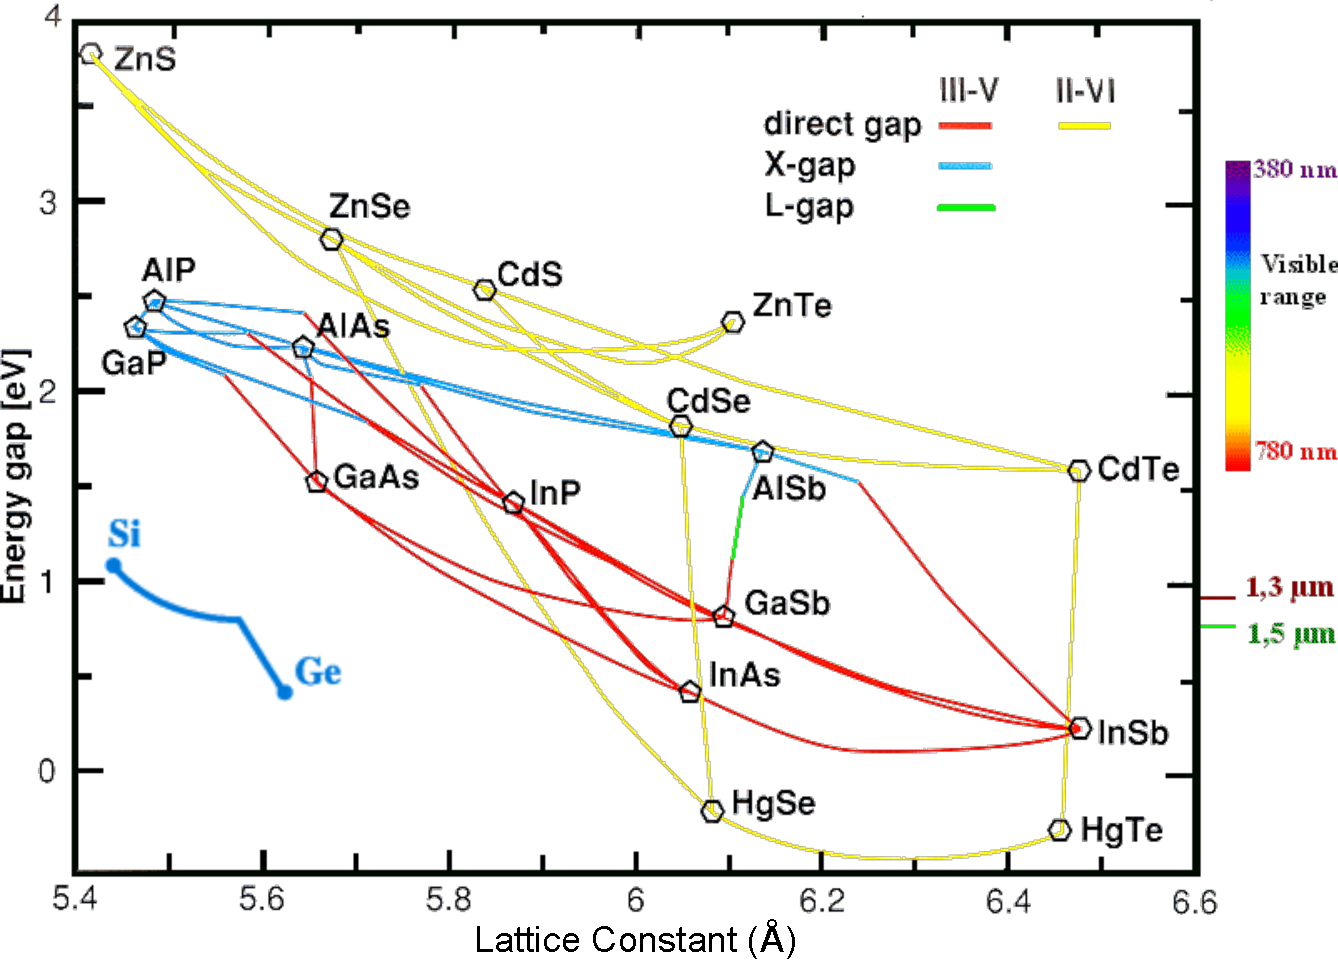
\includegraphics[width=0.9\textwidth]{intro_bandgaps}
    \caption[Bandgap versus lattice constant]{\label{fig:intro_bandgaps}Bandgap versus lattice constant for the most common semiconductors (modified from Helmut\cite{HelmutFoll2013}) (used with permission)}
\end{figure}

Beyond the III-V homologous growth systems, the next most investigated epitaxial process is when these materials are grown on silicon.
In addition to the always-present issue of strain due to the intrinsic lattice mismatch between the III-V family and silicon, the diamond structure of silicon results in an issue of polar (zincblende) on non-polar (diamond) epitaxy\cite{Kroemer1987} where group III and group V atoms cannot differentiate between sites on the silicon surface.
Such site non-specificity has been an issue of great interest to the epitaxy research community resulting in numerous attempts (some successful)\cite{Kroemer1987} to improve growth of such a chemically dissimilar system.

Outside the extensive research into the epitaxy of silicon and the III-V systems, work into epitaxy has mostly been on a material-by-material basis.
Material systems of interest are examined on an issue by issue basis with the goal of producing high quality material for some application, rather than examining the generalized epitaxy phenomenon.
In this work, the goal has been to expand the understanding of epitaxy through an experimental exploration of several model systems which are epitaxial corner cases, and to show other conditions under which high quality epitaxy can occur.
Through this work, two key themes were examined in epitaxial systems, the role of symmetry and the role of energy at epitaxial interfaces.
These themes were examined through investigations into three model material systems, III-V semiconductors on silicon, II-VI semiconductors on crystalline oxides, and noble metals on crystalline oxides.
Investigations into III-V semiconductors on silicon focused on the role of vicinal surfaces, surface reconstructions, and higher order crystal surfaces. Vicinal (or offcut) surfaces of substrates, truncated and reconstructed, were found to have a strong effect on twinning during epitaxial growth, a potential method of improving quality of material growth. (211), a higher order substrate orientation was found to allow accommodation of strain by tilting of a growing epitaxial layer.
Investigations into II-VI semiconductors concentrated on the role of surface reconstructions, and the role of bond strength in epitaxial interfaces. A new epitaxial relationship between temperature stable surface reconstruction and CdTe was observed and atomically modeled, such stable surface reconstructions may offer a new route for lattice matched epitaxial growth. In addition, growths of CdTe on sapphire substrates were found to show a unique liftoff phenomenon, where single crystal films are weakly bonded to the substrate and can be removed while maintaining crystalinity.
Finally, investigations into noble metals on oxide surfaces concentrated on the properties of epitaxy in the weak bonding regime. Epitaxial growth of gold on spinel, a complex oxide, was found to be possible, despite the weak reactivity of both the noble metal and the oxide substrate.
The results from these investigation and the main contribution of this work is to show that epitaxy is possible for symmetrically and chemically dissimilar model systems, and to experimentally examine the implications to epitaxy that such systems have.

\section{Major Themes}
\subsection{Symmetry}
The 2D (and as we shall later see sometimes 3D) interface that separates the epitaxial substrate from the growing crystal has a symmetry relationship which relates the substrate to the crystal.
These surface symmetries are different than the bulk symmetry of the substrate and crystal.
In the simplest treatment of surfaces, the surface of a given substrate is simply a truncation of the crystal in a given orientation, exposing a plane of atoms which then present a subsymmetry of the bulk crystal. Any truncation through a bulk crystal is unstable, since the surface is now exposed to the outside world, and the surface can resolve this instability in a variety of ways.
As will be seen later there are many complications to this model and it is in these complications that we find interesting changes in symmetry, breaks in symmetry and distortions of this 2D surface into a more complex 3D interface.
It is these changes to the surface symmetry, and it's interaction with the growing crystal which have profound and useful implications for epitaxy.
The first major theme investigates the implications of unique interface symmetries, broken symmetries and 3D interfaces on the epitaxial process.

\subsection{Energy}
While symmetry describes the spatial distribution of the landscape presented to a growing crystal, energy describes the magnitude of the effect that landscape has.
Strong energy landscapes cause the symmetry of a given substrate to have it's influence felt strongly, while a weak landscape can have a subtle effect on growth. Whether atoms are bonded via physisorption, covalent bonding, ionic attraction or Van der Walls forces determines the strength of the interface landscape energy.
The energy landscape of the epitaxial interface can vary over a large range, and the role of these strengths has not been examined extensively.
The second major theme of this work investigates the implications of energy landscapes outside the typical heteroepitaxy regime, specifically relating to the weaker energies.

\section{Secondary Themes}
\subsection{Combined Reciprocal Space and Real Space Characterization}
The investigations into epitaxy discussed throughout this thesis have relied upon a variety of techniques to reveal the patterns behind these processes. The most fruitful of the techniques utilized in this work has been the combined use of reciprocal space mapping via 2DXRD and the direct imaging of samples using TEM/STEM. These techniques, when used individually, often lead to ambiguity in the results. STEM/TEM, being a small-area sampling technique can frequently miss information, or cause false interpretations of ``common'' results, when a given sample may be unique or atypical. Similarly, the use of reciprocal space mapping alone gives a picture which convolves all of the data in the sampling area together, providing little insight about its spatial distribution. When these two techniques are combined, the two datasets must be successfully reconciled for a given model of the underlying system to be coherent. Such consistency requirements allow competing explanations to be discriminated from one another based on predictions they make about the data, leading to more complete and less ambiguous models. Such a combination of techniques has also encouraged collaboration, as one cannot be an expert in the operation and interpretation of both systems without compromising the work one originally intended to do.

\part{III-V Materials on Silicon}
\chapter{The Role of Vicinal Surfaces in Epitaxial Twin Formation}
\subsection{Introduction}
Since the microelectronics revolution, Silicon has been a dominant material 
for the production of devices for a variety of applications. Silicon has 
non-ideal properties for a variety of applications but remains dominant due 
to its well-understood processing parameters and large manufacture install 
base, providing economies of scale. The III-V semiconductors offer superior 
properties for a variety of applications when compared to silicon, and are 
actively used in applications were performance is valued above other 
considerations, such as military and space sectors. The goal of integrating 
III-V semiconductors into silicon based microelectronics has spawned extensive 
research into the processing involved to grow or otherwise electronically 
attach these materials with minimal defects.

Under auspices of the ARISE Photovoltaics project, the III-V 
semiconductors GaAs, GaSb, AlSb and InP were grown as thin films under a 
variety of conditions on single crystal silicon substrates, in order to 
examine the growth process and electro-optic properties. The role of the 
varied lattice mismatch, growth parameters, and substrate properties were 
examined and several previously undocumented phenomona were examined due to 
the use of 2DXRD, whose benefits were documented in \cref{sec:2DXRD}.

The formation of epitaxial (or growth) twins was found to be a key area where 
the literature had performed little examination. The role of twins in the 
formation of electronic defect networks, and the effects vicinal (offcut) 
substrates had on their formation were thoroughly examined and a 
explanatory model was developed to explain factors that affect their formation 
and provide proposed routes towards their minimization and 
elimination\cite{Devenyi2011}. This work was completed in close collaboration 
with Ms. Steffi Woo, a Ph.D. candidate in Material Science and Engineering and 
McMaster, with the TEM/STEM work performed exclusively by her and all other 
work being collaborative.

\subsection{Background}
\todo{Should a section covering the background of III-V on Silicon go here, or 
go into the introductory material at the beginning of the thesis}

\subsection{Experimental} \todo{This section is currently copy-pased from 
paper, is this appropriate?}
Semiconductor thin films (GaAs, InP, GaSb, and AlSb) were deposited on nominal 
(001)-oriented ($\pm$0.5$^\circ$) and vicinal Si substrates (offcut 
4.7$^\circ$ ($\pm$0.25$^\circ$) towards [110]) using a SVT Associates 
molecular beam epitaxy (MBE) system. As-received epi-ready wafers were cleaned 
for 1 min in a 4\% HF in deionized (DI) water dip followed by a 30 sec DI 
rinse immediately prior to their insertion into the MBE load-lock. Before film 
deposition, both the nominal and vicinal Si(001) substrates underwent a 15 min 
degassing procedure at 350~$^\circ$C followed by a thermal treatment at 
800~$^\circ$C for up to 5 min, in order to reconstruct the Si surface into 
single domain 
terraces\cite{NeergaardWaltenburg1995,S1991,Sakamoto1986,Pehlke1991}. A small 
number of single steps are expected to remain on vicinal substrates, a higher 
number on nominal substrates because of the larger terrace length. Growth 
conditions followed established 
protocols\cite{Akahane2004,Balakrishnan2006a,Fischer1986} and yielded 
comparable rocking curve full-width half-maximum for the [004] reflection 
using double crystal X-ray diffraction. AlSb thin films were grown to a 
thickness of 550~nm with a 20~nm GaSb capping layer to avoid oxidation. GaAs 
thin films was grown to a thickness of 600~nm and GaSb to a thickness of 
500~nm. InP samples were grown at 470~$^\circ$C with a V/III flux ratio of 2 
at a growth rate of 1 $\mu m$/hr, resulting in a thickness of 600~nm. Double 
crystal X-ray and TEM data also revealed that all films are fully relaxed by a 
network of interfacial misfit dislocations\cite{Vajargah2011}. GaSb samples 
were grown in the presence of a 5 nm AlSb buffer layer, as prescribed by 
Akahane \textit{et al}.\cite{Akahane2004}.

Stereographic pole figures were generated for each sample using 2DXRD 
techniques. A Bruker SMART 6000 CCD detector on a Bruker 3-circle D8 
goniometer (Bruker AXS Inc., Madison, WI) with a Rigaku RU-200 rotating anode 
X-ray generator (Rigaku MSc, The Woodlands, TX) and parallel-focusing 
monochromator optics was used for the data collection. Scans were taken with 
the detector centered on the (111) 2$\theta$ of the material of interest and 
the sample rotated through 360$^\circ$ in 0.5$^\circ$ increments about the 
surface normal of the sample. A 1D integration of all frames was used to 
determine the combined width of the (111) peaks using MAX3D software (McMaster 
University)\cite{Britten2007}. The peak width was then used to integrate (111) 
reflections from all frames, including a background and absorption correction 
for the corresponding material with GADDS (Bruker-AXS) software, resulting in 
a pole figure. Pole intensities were obtained from pole figures using a 
circular integration cursor with a 10 pixel radius which was centered on the 
pole so as to maximize the total intensity captured. All pole intensities were 
corrected for structure factor and frame exposure times.

For each sample two \{110\} TEM cross-sections were prepared, one parallel to 
the [110] miscut direction and the other perpendicular. The specimens were 
prepared by the standard procedure of mechanical polishing, dimpling, and 
ion-milling (4 keV Ar-ions at an incident angle of $\pm$4$^\circ$ using a 
liquid nitrogen cold stage for InP) until perforation. Crystallographic 
information of the epitaxial layer was obtained using diffraction contrast 
imaging with a Philips CM12 conventional transmission electron microscope 
(TEM) operated at 120 kV and equipped with a LaB$_6$ filament. In addition, 
electron diffraction analysis was performed using selected area electron 
diffraction (SAD).
\subsection{Results}
2DXRD measurements performed on as-grown thin films indicated a bulk 
orientation of the material consistent with epitaxial alignment with the 
single crystal silicon substrate. The pole figures generated from 2DXRD data, 
such as \cref{fig:twins_pole_example} also contained a number of other peaks 
at reduced intensity indicating other orientations of the material of interest 
other than the bulk orientation. In order to develop a comprehensive picture 
of the distribution of the grown thin films, simulated pole figures were 
examined in an attempt to generate a composite pole figure which qualitatively 
matched the figures generated from data. Based on these simulations, the 
simulated pole figure \cref{fig:twins_sim_polefigure} was developed, 
indicating that the thin films consisted of a bulk epitaxial phase, and four 
primary twin phases, along with secondary twin phases (not shown). The primary twins form 
along (111), (1$\overline{1}$1) ($\overline{1}\overline{1}$1) and ($\overline{1}$11) 
habit planes.
\begin{figure}
    \begin{subfigure}[b]{0.5\linewidth}
        \centering
        \missingfigure{Representative Single Pole Figure}
        \caption{A representative pole figure of GaAs grown on nominal (100) 
        Silicon\label{fig:twins_pole_example}}
    \end{subfigure}
    \begin{subfigure}[b]{0.5\linewidth}
        \centering
        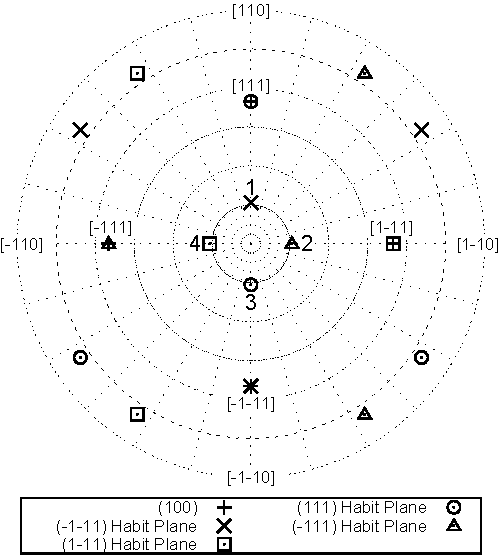
\includegraphics[width=\textwidth]{twins_sim_polefigure}
        \caption{Simulated III-V on silicon pole figure. Unique markers are used 
        for later intensity measurements.\label{fig:twins_sim_polefigure}}
    \end{subfigure}
    \caption{\label{fig:polefigure_example}Represenative pole figure and simulated pole 
    figure}
\end{figure}

Growths of III-V thin films were performed on vicinal substrates due to the established 
literature indicating the ability of atomic height steps formed by such substrates to 
overcome the polar-on-non-polar growth problem\cite{Kroemer1987}. The pole figures 
generated for thin films grown on vicinal substrates were found to have a distinctive 
asymmetry in the intensity distribution of the peaks associated with twinned orientation, 
when compared to the thin films grown on nominal silicon substrates. The pole figures for 
both nominal and vicinal pole figures for the III-V thin films are shown in 
\cref{fig:twins_polefigure}.

\begin{figure}
    \centering
    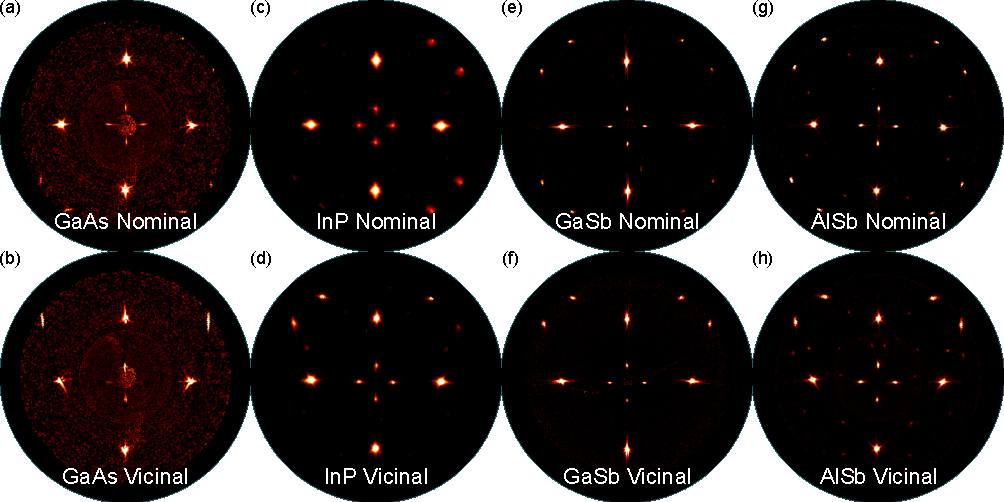
\includegraphics[width=\textwidth]{twins_polefigure}
    \caption{Stereographic \{111\} pole figures generated from 2DXRD show a bulk (100) 
    phase plus four twinned variants as identified in \cref{fig:twins_sim_polefigure}. 
    Twin variant intensity is asymmetric for vicinal 
    substrates.\label{fig:twins_polefigure}}
\end{figure}
\chapter{Tilted Epitaxy on 211 Oriented Substrates}
\section{Introduction}
In parallel to the investigations of vicinal (100) substrates, the ARISE project investigated alternative substrate orientations including (111) and (211). While the results of (111) substrates were uninteresting, growth of thin films on (211) substrates demonstrated a number of interesting properties. Most interesting amongst these was the spontaneous tilting of thin films grown on top of (211) oriented silicon substrates. Such tilting had been remarked upon previously in literature,  but no comprehensive examination of its origins or relationship to material parameters had been examined.

In this work, also done in close collaboration with Ms. Steffi Woo, the spontaneous 
tilting of thin films grown on (211) oriented silicon substrates was examined. The 
effects of the naturally asymmetric substrate was found to cause a tilt of the growing 
thin film in order to minimize the strain across the interface. Using this idea of 
projected strain minimization across the interface, a model was developed which predicted 
the tilt as a function of intrinsic lattice mismatch between the substrate and thin film. 
Examination of the reports of thin film tilting in literature showed the model 
successfully calculated tilt for a large number of material systems and made predictions 
for those systems for which no measured values had been reported.
\section{Background}
The (211) orientation of non-polar semiconductor substrates, most notably silicon, has a number of beneficial properties. Of most relevance to the epitaxy of thin films on Si(211) substrates is the occurrence of two energetically non-equivalent lattice sites on the surface, without the need for surface reconstruction.\cite{Wright1982} These two non-equivalent lattice sites offer preferential nucleation locations for the individual adatoms during growth of polar (group III-V and II-VI) semiconductors. Such preferred nucleation is proposed to eliminate the occurrence of anti-phase domains (APDs) during the growth of polar semiconductors\cite{Wright1982} while also maintaining the interface neutrality condition of h$\pm$k$\pm$l$=$0.\cite{Wright1982} The intrinsic asymmetry of the (211) surface is also expected to influence the formation of epitaxial twins during growth\cite{Devenyi2011}. Si(211) substrates have been used to produce the highest quality CdTe\cite{Zhao2011}, ZnTe\cite{Wang2011a} and HgCdTe\cite{Dhar1997a} despite large lattice mismatches of 19.4\%, 12.3\%, and 19.1\%, respectively. 

Thin films grown on (211) substrates have been previously observed in literature to have a tilted epilayer orientation relative to the substrate.\cite{Zhao2011,Wang2006,Dhar1997a,Lange1991,Nakamura1992} The tilt phenomenon has been attributed to a number of causes by different authors including the glide and interactions of misfit dislocations \cite{Olsen1975,Riesz1994,Ayers1991,Johnson2011} and localized distortion of the lattice at the interface.\cite{Sasaki1992} The mechanisms proposed thus far have been unsuccessful at predicting the tilt of mismatched epilayers over large range of mismatch (0--20\%) found in III-V and II-VI material systems. A phenomenon intimately intertwined with tilted epitaxy is ``dual epitaxy'', observed by numerous authors\cite{Li1995a,Nakamura1992,Rujirawat1998,Lange1991} that mismatched CdTe on GaAs(211) epitaxy can result in films growing in a twinned orientation, combined with a tilt; such that the (133) planes make up the epilayer surface and are parallel to the substrate (211) planes. The tilt component of dual epitaxy is same tilt phenomenon examined here.

\section{Experimental}
GaSb thin films were deposited on nominal (211)-oriented Si substrates, according to our 
previously published procedures\cite{Devenyi2011}, at 600, 640 and 500{\degree}C. Two 
dimensional X-ray diffraction (2DXRD) frames were captured for stereographic pole figure 
analysis and crystallographic indexing as per Devenyi \textit{et al.}\cite{Devenyi2011}.
\begin{figure}
    \centering
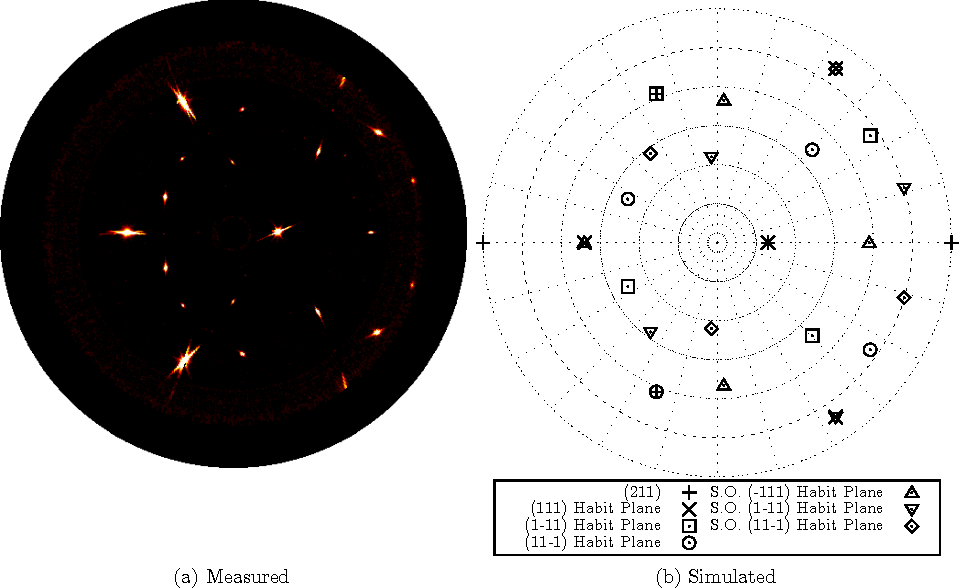
\includegraphics{211_polefigure}
\caption{\label{fig:211_polefigure}a) 2DXRD Stereographic pole figure and b) accompanying modelled pole figure, identifying the origin of each peak in the pole figure from the bulk or one of six twin variants. Overlapping peaks indicate twinning habit planes. Outermost poles are partially visible due to experimental limitations. Streaking in peaks is due to instrumental broadening. (S.O. = second-order twinning).}
\end{figure}
\section{Results}
2DXRD data was processed into a GaSb (111) pole figures as shown in FIG.~\ref{fig:211_polefigure}, representing a stereographic projection of all $<$111$>$ spacings present in the GaSb epilayer. Modeling (as per Devenyi \textit{et al.}\cite{Devenyi2011})\ of the poles present indicate that there are seven phases of GaSb, the bulk (211) orientation of GaSb and six twin variants, three first-order twins and three second-order twins from the twin variant with (111) habit plane, with 58\%, 21\% and 2\% of the intensity (and hence volume fraction) present in the twinned orientation for the films presented here. Volume fractions were determined by integration of the sum of intensity of unique (111) X-ray peaks from all twinned orientations, and divided by total intensity of all unique (111) reflections (sum of bulk and twin intensities), performed using \textit{Bruker GADDS}. There are two distinct nomenclatures used in literature to describe phases present in epitaxial films.\cite{Kim2010a,Lange1991,Johnson2011,DeLyon1995} One method describes the crystallographic direction which is normal to the surface for each phase, while the other (which the authors choose to employ here) describes the nature of the crystallographic orientation relationship between the secondary phases with respect to the orientation of the substrate. Where reference is made to literature using the first, descriptions will be translated into the second for ease of comparison.

Indexing of the crystal unit cells present in the film was performed using \textit{Bruker APEXII} single crystal refinement software, to obtain orientation matrices for the Si substrate as well as the seven GaSb phases. The bulk thin film orientation matrix was then compared to the substrate matrix and a tilt calculated using \textit{orilib} a crystal orientation calculation library, yielding a tilt of 2.65\degree, 2.55\degree and 2.40\degree $\pm$ 0.2\degree about the [01$\overline{1}$] direction towards [$\overline{1}$11], these values are indistinguishable within experimental error. The (111) habit plane twin formed in these films is also tilted with respect to the substrate, by the same angle as the bulk, this is expected by crystallography, since this twinned orientation shares extended interfaces with the bulk orientation.
\begin{figure}
    \centering
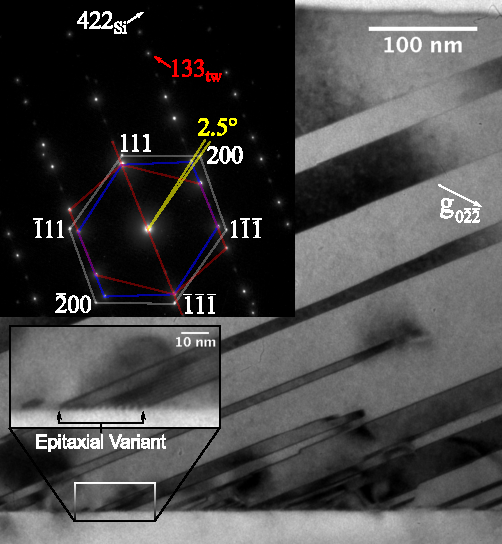
\includegraphics{211_tem}
\caption{\label{fig:211_tem}Conventional TEM image of the (0$\overline{1}$1) cross section, with inset diffraction pattern of the epitaxial and (111) habit plane twin variant in blue and red, respectively, and inset higher-magnification of the epitaxial variant showing misfit dislocations.}
\end{figure}

Two transmission electron microscopy (TEM) cross-sections were prepared, in orthogonal directions of [0$\overline{1}$1] and [1$\overline{1}\overline{1}$]. The specimens were prepared by conventional mechanical polishing and ion milling, and examined as described in Woo \textit{et al.}\cite{Woo2012} Conventional TEM imaging of the (0$\overline{1}$1) cross-section of the epilayers, combined with the selected area electron diffraction (SAED) pattern of the [0$\overline{1}$1] zone axis as shown in FIG.~\ref{fig:211_tem} confirms the presence of microtwins with (111) habit planes. These microtwins are observed in the perpendicular (1$\overline{1}\overline{1}$) cross-section as large bands lying parallel to the interface over a long-range, alternating with the epitaxial variant (not shown). The observed misorientation between the GaSb and Si reflections in the [0$\overline{1}$1] SAED pattern also indicate a tilted epilayer (both epitaxial and twin variants) with a tilt of 2.54$^\circ \pm 0.2^\circ$ towards the [$\overline{1}$11] direction. The 133 reflection of the twinned GaSb nearly coincides with the Si substrate normal 422 reflection. The GaSb twin variant can be differentiated in real space by selective dark-field imaging formed using one of the twinned reflection spots. The jagged features at the GaSb/Si interface (seen in detail in the inset of FIG.~\ref{fig:211_tem}) only belong to the epitaxial variant. This is indicative of the presence of misfit dislocations at the portions of the interface where the epitaxial region meets the substrate, as characterized by Vajargah \textit{et al.}\cite{Vajargah2011b}
\section{Discussion}
Analysis using an atomic ball-and-stick model, along with trigonometric modelling of lattice plane spacing, can be used to demonstrate that the tilted epitaxy reduces the projected in-plane lattice strain along one dimension for the GaSb/Si system. FIG.~\ref{fig:211_model} shows the alignment of planes present in the epitaxial and twinned variants of the GaSb epilayer. The Si(111) plane spacing (in red) at an angle of 19.471\degree to the Si(211) surface is aligned to the GaSb(111) plane spacing (in blue), by a tilt of 2.50\degree in the epilayer. The relationship describing zero projected strain condition between these planes across the interface is described in EQN.~\ref{eqn:211_epi} for the case of $a_{Sub} = a_{Si}$ and $a_{Film} = a_{GaSb}$, where $\delta$ is the tilt angle. This relationship (dot-dash line) also applies over the full range of common heteroepitaxial lattice mismatches grown on (211) substrates, from GaP/Si to CdTe/Si, as shown in FIG.~\ref{fig:211_data}.
\begin{gather} 
 \frac{ a_{film}}{\sqrt{3} \sin(19.471^\circ + \delta)} = \frac{a_{Sub}}{\sqrt{3}\sin(19.471^\circ)} \label{eqn:211_epi}\\
 \frac{ a_{film}}{2\sin(74.207^\circ + \delta)} = \frac{ a_{Sub}}{\sqrt{3}}   \label{eqn:211_twin}
\end{gather}
\begin{figure}
    \centering
\includegraphics{211_model}
\caption{\label{fig:211_model}Ball-and-stick atomic model of a triple junction of the epitaxial orientation, twinned orientation (with (111) habit plane in blue), and the Si(211) surface. Geometrical alignment of the atomic planes as described by EQNs.~\ref{eqn:211_epi} and \ref{eqn:211_twin} are also shown in red/blue and black, respectively. Terrace (T) and edge (E) atom labels denote the two non-equivalent surface sites.}	
\end{figure}
\begin{figure}
    \centering
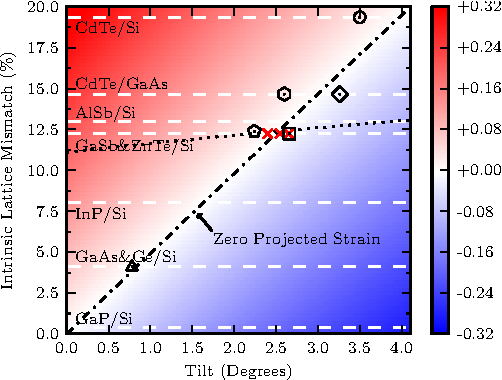
\includegraphics{211_data}
\caption{\label{fig:211_data}Colormap showing the projected strain as a function of 
intrinsic lattice mismatch and positive tilt angle of an epitaxial film, computed from 
EQN.~\ref{eqn:211_epi} with the zero projected strain contour highlighted (dot-dash 
line). The dotted line also overlays EQN.~\ref{eqn:211_twin}. Experimental data points 
from this work ($\times$), Ref.~\textcite{Zhao2011} ($\odot$), Ref.~\textcite{Wang2011a} 
($\boxdot$), Ref.~\textcite{Johnson2011} ($\Diamond$, $\bigtriangleup$) and 
Ref.~\textcite{smith2012_znte,smith2012_gaas} ($\pentagon$, $\varhexagon$) are shown, 
indicating good agreement with measured tilts of thin films. Common heteroepitaxial 
systems are also highlighted. Close lattice mismatches are merged for figure clarity.}
\end{figure}
In the twinned orientation, the Si($\overline{1}$11) plane spacing is aligned to the projection of the GaSb(200)$_{tw}$ plane spacing (both in black) onto the GaSb/Si interface, by a tilt of 2.22\degree. The geometrical constraints of these planes can be described by the relations as expressed in EQN.~\ref{eqn:211_twin}. The line of zero projected strain for the twinned region is also shown in FIG.~\ref{fig:211_data} (dotted line). The applicability of EQN.~\ref{eqn:211_twin} is considerably more limited across heteroepitaxial systems, as the constraints described by EQN.~\ref{eqn:211_epi} also needs to be simultaneously satisfied as extended interfaces are shared. However, an equivalent relationship describing another set of planes for other lattice mismatches may replace the relationship described by EQN.~\ref{eqn:211_twin}. The proposed ball-and-stick atomic model (FIG.~\ref{fig:211_model}) also shows that the Ga- and Sb-atoms in the twinned variant are perfectly registered with the terrace (T) and edge (E) atoms of the Si substrate. The epitaxial variant interface is significantly distorted, and the same atomic registration of Ga- and Sb-atoms to the underlying Si substrate does not occur, however the projected sublattice is still aligned. This correlates well with the misfit dislocations observed at the GaSb/Si interface in the inset of FIG.~\ref{fig:211_tem}.

For general case of an epilayer with unknown twin volume-fraction, the tilt is bounded by competing factors of minimizing strain in both the epitaxial and twinned variants (as in GaSb on Si), with the projected strain effectively minimized at the volume-fraction weighted average of the two tilts. For GaSb with 58\%, 21\% and 2\% twin fraction, the predicted tilts are 2.493\degree, 2.498\degree and 2.500\degree. This small variation in tilt angle is due to the steeper slope of EQN.~\ref{eqn:211_epi}, thus its contribution dominates the weighted average. The intrinsic +12.2\% lattice mismatch between GaSb and Si is minimized, however there are localized strain variations between the epitaxial and twinned regions. For a film with 58\% twin, the projected (111) d-spacing in the epitaxial region is +0.03\% (in compression), while the projected GaSb(200) and Si($\overline{1}$11) d-spacing in the twinned region is -0.12\% (in tension). Thus, the proposed driving force for the tilted epilayer during growth is the minimization of lateral strain of close-packed (111) planes (red/blue planes in FIG.~\ref{fig:211_model}), in one dimension within the two-dimensional projected interface net.

In addition to accounting for the tilt observed for GaSb on Si, this model predicts the tilts observed in several other material systems. The growth of CdTe on Si(211) and GaAs(211) is a common use to buffer the growth of HgCdTe for detector applications. Several authors\cite{Triboulet2009,Yu1999,Lange1991} published results which indicate CdTe epilayers which are tilted in the range of 3.5\degree on Si(211)\cite{Zhao2011} and 3.26\degree on GaAs(211)\cite{Johnson2011}, about the [01$\overline{1}$] direction towards [$\overline{1}$11]. The direction and magnitude reported by those authors agrees well with the tilt of 3.97\degree and 3.00\degree, respectively, as predicted by this model. Discrepancy between the predicted and reported value of tilt is expected to be partially due to the presence of twinning in the epilayer, along with uncertainty in the reported values.

ZnTe is often used as an intermediate buffer epilayer, prior to the growth of CdTe and HgCdTe on Si(211).\cite{Zhao2011,Dhar1997a} Wang \textit{et al.}\cite{Wang2011a} published results which indicate epilayer tilts in the range of 2.66\degree while Smith \textit{et al.}\cite{smith2012_znte} reports tilts of 2.24\degree. This is in good agreement to the predicted value of 2.50\degree obtained from the proposed model. The good matching between our predicted and the reported values of tilt in ZnTe on Si(211) is expected to be due to the substantially low degree of twinning observed.

The model also makes a prediction of the tilt expected from the growth of GaAs on Si(211), a value of 0.83\degree is predicted. A tilt of 0.781\degree is reported by Johnson \textit{et al.}\cite{Johnson2011} when grown alone, and 0.835\degree when capped subsequently with CdTe, again demonstrating good agreement with the model.

For the systems AlSb/Si, InP/Si and GaP/Si, the model predicts tilt angles of 2.65\degree, 1.64\degree and 0.07\degree. Measurements of these material systems are expected to yield tilts that quantitatively follow this model.
\section{Implications for Symmetry and Energy at Epitaxial Surfaces}
The natrually asymmetric (211) surface of cubic non-polar semiconductors offers a alternative route to breaking the symmetry for epitaxial growth. The (211) surface offers two unique properties which can enhance nucleation and growth of lattice mismatched thin films, it's asymmetric surface offers a energy landscape offering different bonding locations, and it's surface has a naturally stepped nature.

The two non-equivalent surface sites present on an unreconstructed (211) surface offer an energy landscape which encourages the nucleation of the polar adatoms. Such a preferred nucleation of adatoms into the two non-equivalent sites results in the natural elimination of anti-phase-domains.

The surface of (211) oriented semiconductors, in addition to having non-equivalent sites, also has a naturally asymmetric surface, consisting of 
\part{Semiconductors on Oxide Substrates}
\chapter{CdTe Growth on Sapphire Substrates and Liftoff Phenomenon}
\section{Introduction}
The growth of CdTe on oxide substrates, specifically single crystal sapphire, has been a 
region of great interest for the Preston research group. Work has been published on 
optimization of growth parameters, the role of lattice constants, and the optical 
properties of the resulting thin films\cite{svetlana-work,stephen-paper}.

While the work investigating the growth parameters and properties of the resulting thin 
films has progressed to a high level, relatively less investigation has been focused on 
explaining the surprising success that has been achieved with this material system. With 
a relative lattice mismatch of 3.xx\% between CdTe and sapphire, a difference in the 
crystallographic space group (cubic CdTe versus hexagonal sapphire), and a vast chemical 
difference (high ionicity semiconductor CdTe versus complex oxide sapphire), the high 
quality single crystal nature of the grown thin films is far from expected.

In this work investigating the CdTe on sapphire heteroepitaxial material system, the 
unexpected high quality growth is examined through the lens of symmetry and energy at the 
epitaxial 
interface. These examinations reveal theoretical support for an explanatory model of the 
epitaxial alignment 
and defects present in CdTe thin films. These examinations also reveal the previously 
undocumented and highly surprising result that CdTe is not bonded nearly as strongly as 
expected to the sapphire substrates after epitaxial growth, resulting in the 
technologically relevant liftoff phenomenon. The liftoff phenomon is examined and its 
resulting freestanding thin films are characterized. This liftoff phenomon has been 
discovered to be significantly robust as to apply for a provisional patent\cite{patent}. 
This work was completed in collaboration 
with Mr. Stephen M. Jovanovic (growths), Dr. Kristoffer Mienander (DFT, surfaces) and Ms. 
Steffi Woo (TEM), and relies on prior work by Dr. Robert Hughes and Dr. Svetlana Neretina.

\section{Background}
CdTe is a cubic semiconductor (a = 6.14xxx) with a very strong propensity to grown 
(111)-up, that is 
alternating layers of cadnimum and telurium, regardless of the structure of the 
underlying substrate. Thus the key requirement for the growth of quality single crystal 
thin films is to control the nucleation and in-plane orientation. \textalpha-Al$_2$O$_3$ 
(sapphire) 
is a rhobehedral complex oxide (a = xxxx, c = yyy), which presents a hexgonal surface net 
on its c-plane surface. As had been previously investigated by the Preston research 
group, the (110) diagonal of CdTe matches to a lattice constant of sapphire to within 
3.xx\%, providing a geometric template for the epitaxial alignment of (111)-up on the 
c-plane surface. While the c-plane sapphire offers an epitaxial template for the CdTe, 
the mismatch of cubic on hexagonal symmetries offers two equivalent orientations for the 
CdTe crystal, as shown in \cref{fig:cdteliftoff_geometry}.
\begin{figure}
    \centering
    \missingfigure{Triangle on Hexagon Fit}
    \caption{\label{fig:cdteliftoff_geometry}Geometric model of cubic CdTe crystal 
    structure fit on hexagonal c-plane sapphire surface}
\end{figure}
Despite the geometric equivalence of two orientations of cubic on hexagonal symmetry, 
growths done by this research group have resulted in a single orientation of CdTe on the 
sapphire surface. Previous work by this research group attempted to explain the preferred 
orientation through experiments in the modification of sapphire\cite{Neretina2009b}, 
suggesting that the energy considerations at the surface play a key factor in epitaxy.
\section{Experimental}
CdTe thin films were deposited on single crystal c-plane \textalpha-Al$_2$O$_3$ $\pm$ 
0.5\degree wafers, obtained from MTI Crystals Inc and diced into 12 mm $\times$ 12 mm 
squares. Prior to deposition, substrates were solvent cleaned in an ultrasonic bath. 
Samples were loaded into a custom pulsed laser deposition chamber at a base pressure of 
1x10E-7 Torr and in-situ annealed at 450\degree\celsius for 30 minutes. CdTe thin films 
were deposited by pulsed laser deposition using a GSI Lumonics IPEX-848 KrF excimer laser 
with a wavelength of 248 nm. Pulses from the laser were focused and rastered radially 
onto a rotating CdTe 2.54 cm diameter target with a spot size of 4.25 
mm\textsuperscript{2} and average 
energy density of 1.8 J/cm\textsuperscript{2}. The CdTe 5N (99.999\%) pressed powder 
target obtained from 
Princeton Scientific was stoichiometric and undoped. During growth samples were kept at a 
nominal temperature of 300\degree\celsius via a Pt-Rh thermocouple on the growth furnace 
surface. 
Films were grown to a thickness of 100 nm, as determined by optical and stylus 
profilometry.

Structural information was obtained using 2DXRD techniques. A Bruker SMART6000 CCD 
detector on a Bruker 3-circle D8 goniometer with Rigaku RU-200 rotating anode X-ray 
generator and parallel-focusing mirror optics were used for the data collection. 2DXRD 
data was processed into pole figures using Bruker GADDS.
\section{Results and Discussion}
CdTe thin films had been previously thoroughly structurally characterized via 2DXRD, AFM 
and TEM. As such, one of the next steps to fully characterize the CdTe thin films was to 
produce larger uniform films\cite{stephen-thesis} and to electrically characterize films 
via resistivity and hall effect. As part of this investigation, lithographic patterning 
of Pt contacts was performed to create van der pauw geometry. Upon performing the acetone 
soak, as the photoresist dissolved, and the metal film floated off the sample, it 
remained in one piece, lifting off the areas of CdTe that were in contact with the metal from the epitaxial substrate. 
For a sample that had been previously characterized to be single crystal, this result was 
unexpected, as all that was required for this liftoff was an ultrasonic bath.
\begin{figure}
    \centering
    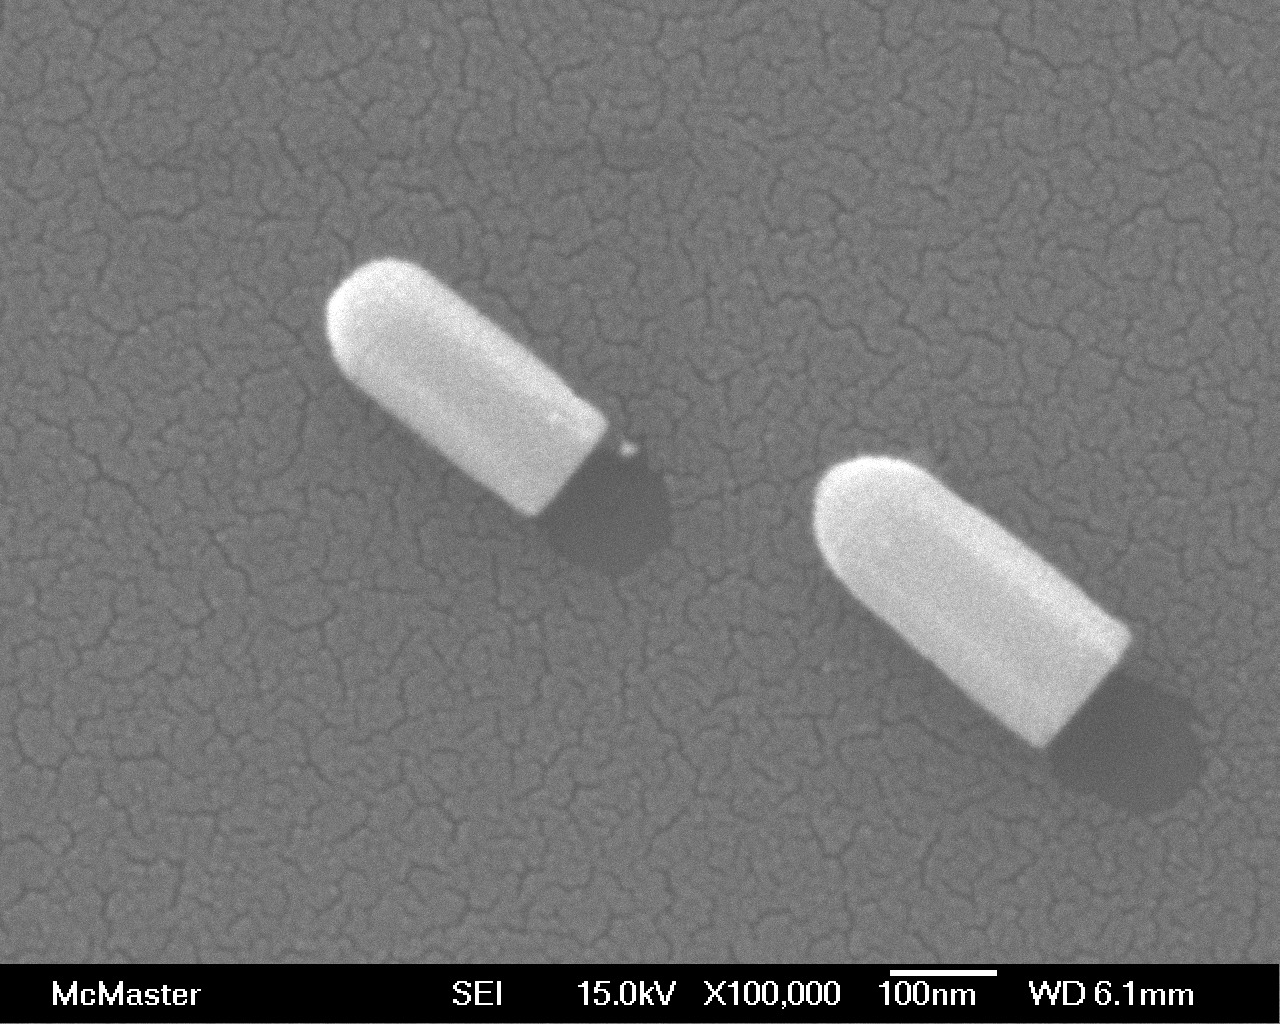
\includegraphics[width=0.8\textwidth]{cdteliftoff_nanowires}
    \caption{\label{fig:cdteliftoff_nanowires}}
\end{figure}
This weak bonding phenomenon had been previously hinted at when CdTe nanowires were 
observed in SEM to have toppled in place, as shown in \cref{fig:cdteliftoff_nanowires}, a 
event that could not have happened unless the bond strength with the interface was very 
weak.

After the discovery of the liftoff phenomenon with lithographic patterning, simpler 
methods of liftoff were attempted. Strong adhesive tapes were found to successfully 
remove thin films with a simple mechanical peeling motion. While the tape peeling was 
effective, the large curvatures cause cleaving and breakage in the lifted off film. 
Adhesive epoxies were attempted and found to provide a more rigid carrier, eliminating 
cleaving and breakage. Yields of liftoff are highly dependent on the quality of bonding 
to the CdTe surface, clean surfaces and effective adhesives are key. Numerous other 
bonding methods were tested including optical element adhesive, polymer films and the 
simplification of liftoff by the addition of LN\textsubscript{2} as thermal shock. The generalized adhesive based liftoff process is shown in \cref{fig:cdteliftoff_process}
\begin{figure}
    \centering
    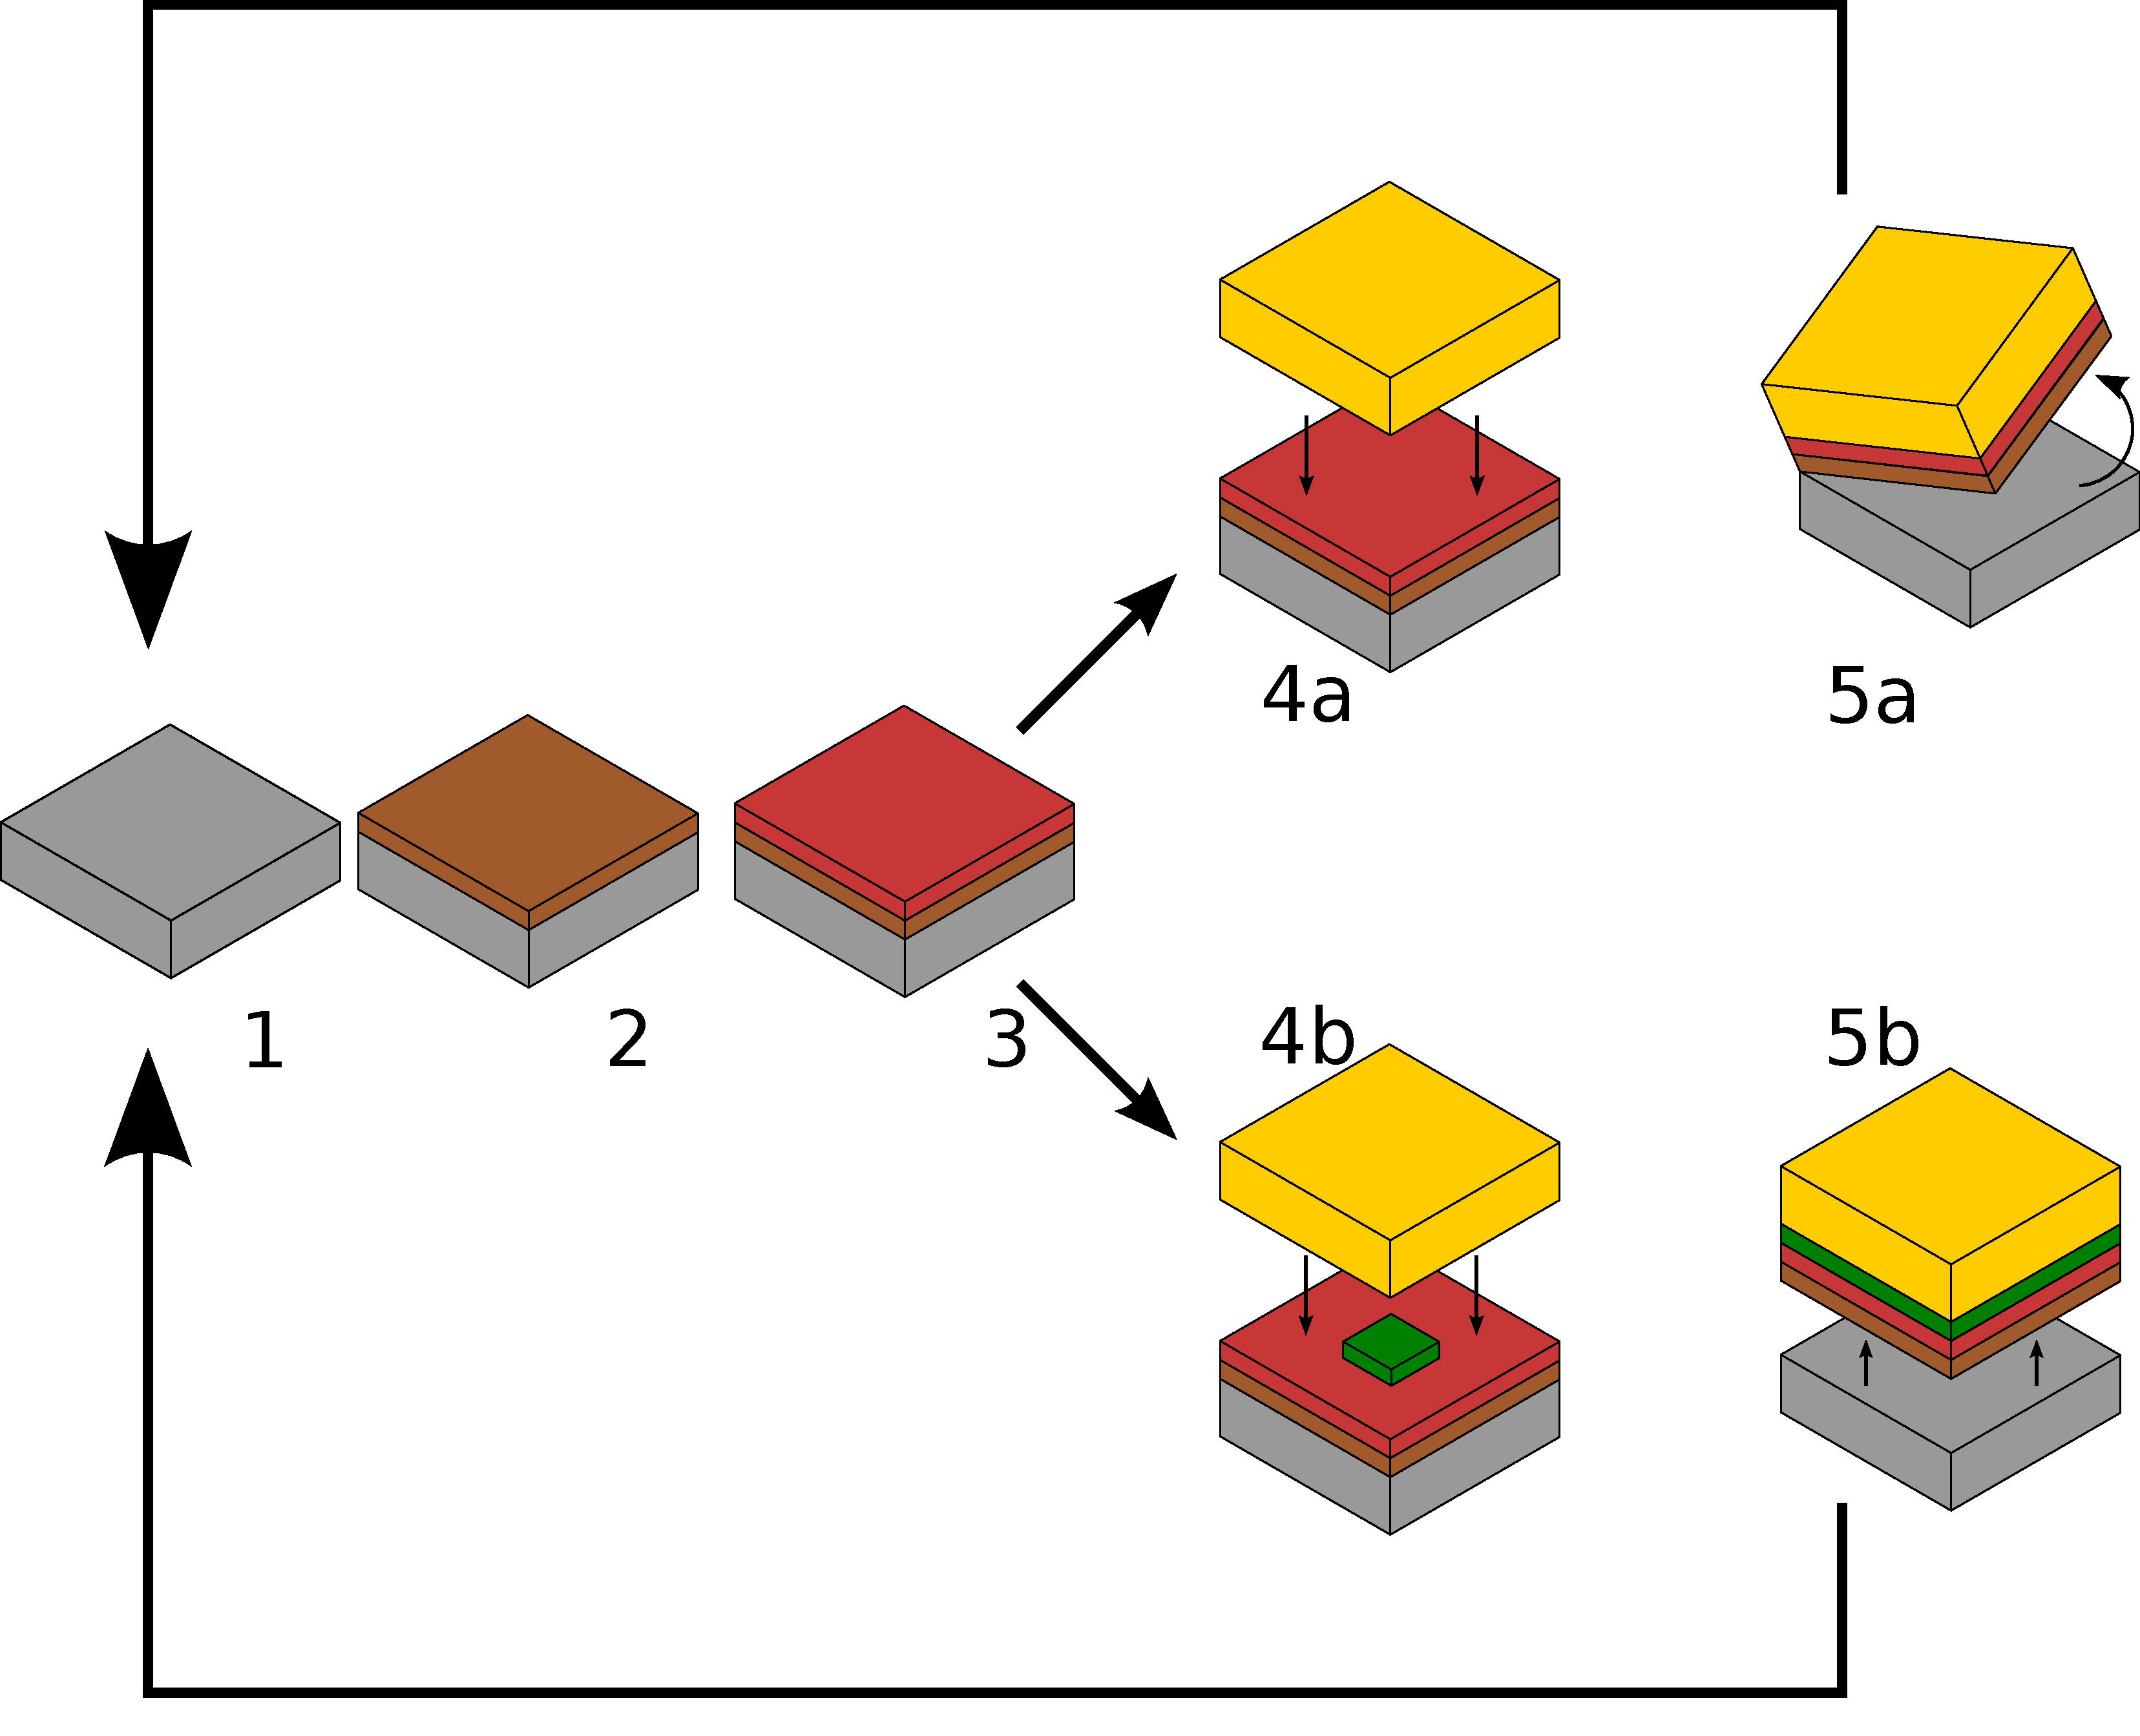
\includegraphics[width=\textwidth]{cdteliftoff_process}
    \caption{\label{fig:cdteliftoff_process}The generalized CdTe liftoff process}
\end{figure}
The flexible non-conductive liftoff carriers offered a first step to producing 
freestanding thin films, but electrical contact to the films is a key property in order 
to yield devices. To this end, thin films were coated with metal, first platinum (a known 
CdTe contact material) and then copper, in order to create a temperature stable surface. 
Samples were then wetted with solder paste and placed metal side down onto a copper 
surface, and thermally cycled through a solder reflow curve, as shown in 
\cref{fig:cdteliftoff_process}b. Upon removal from the oven, the films were found to have bonded to the copper surface and spontaneously lifted off from the original sapphire substrate. These experiments have demonstrated that the production of freestanding thin films by the liftoff phenomon is remarkably simple and straightforward.

Concurrent to investigations into the production of freestanding thin films via the liftoff process, the obvious question arose as to the properties of these films when compared to those attached to the epitaxial substrate. 2DXRD measurements were undertaken on thin films before, \cref{fig:cdteliftoff_F22_attached} and after \cref{fig:cdteliftoff_F22_released}, liftoff processing using two part epoxy.
\begin{figure}
    \centering
    \begin{subfigure}[b]{0.4\textwidth}
        \centering
        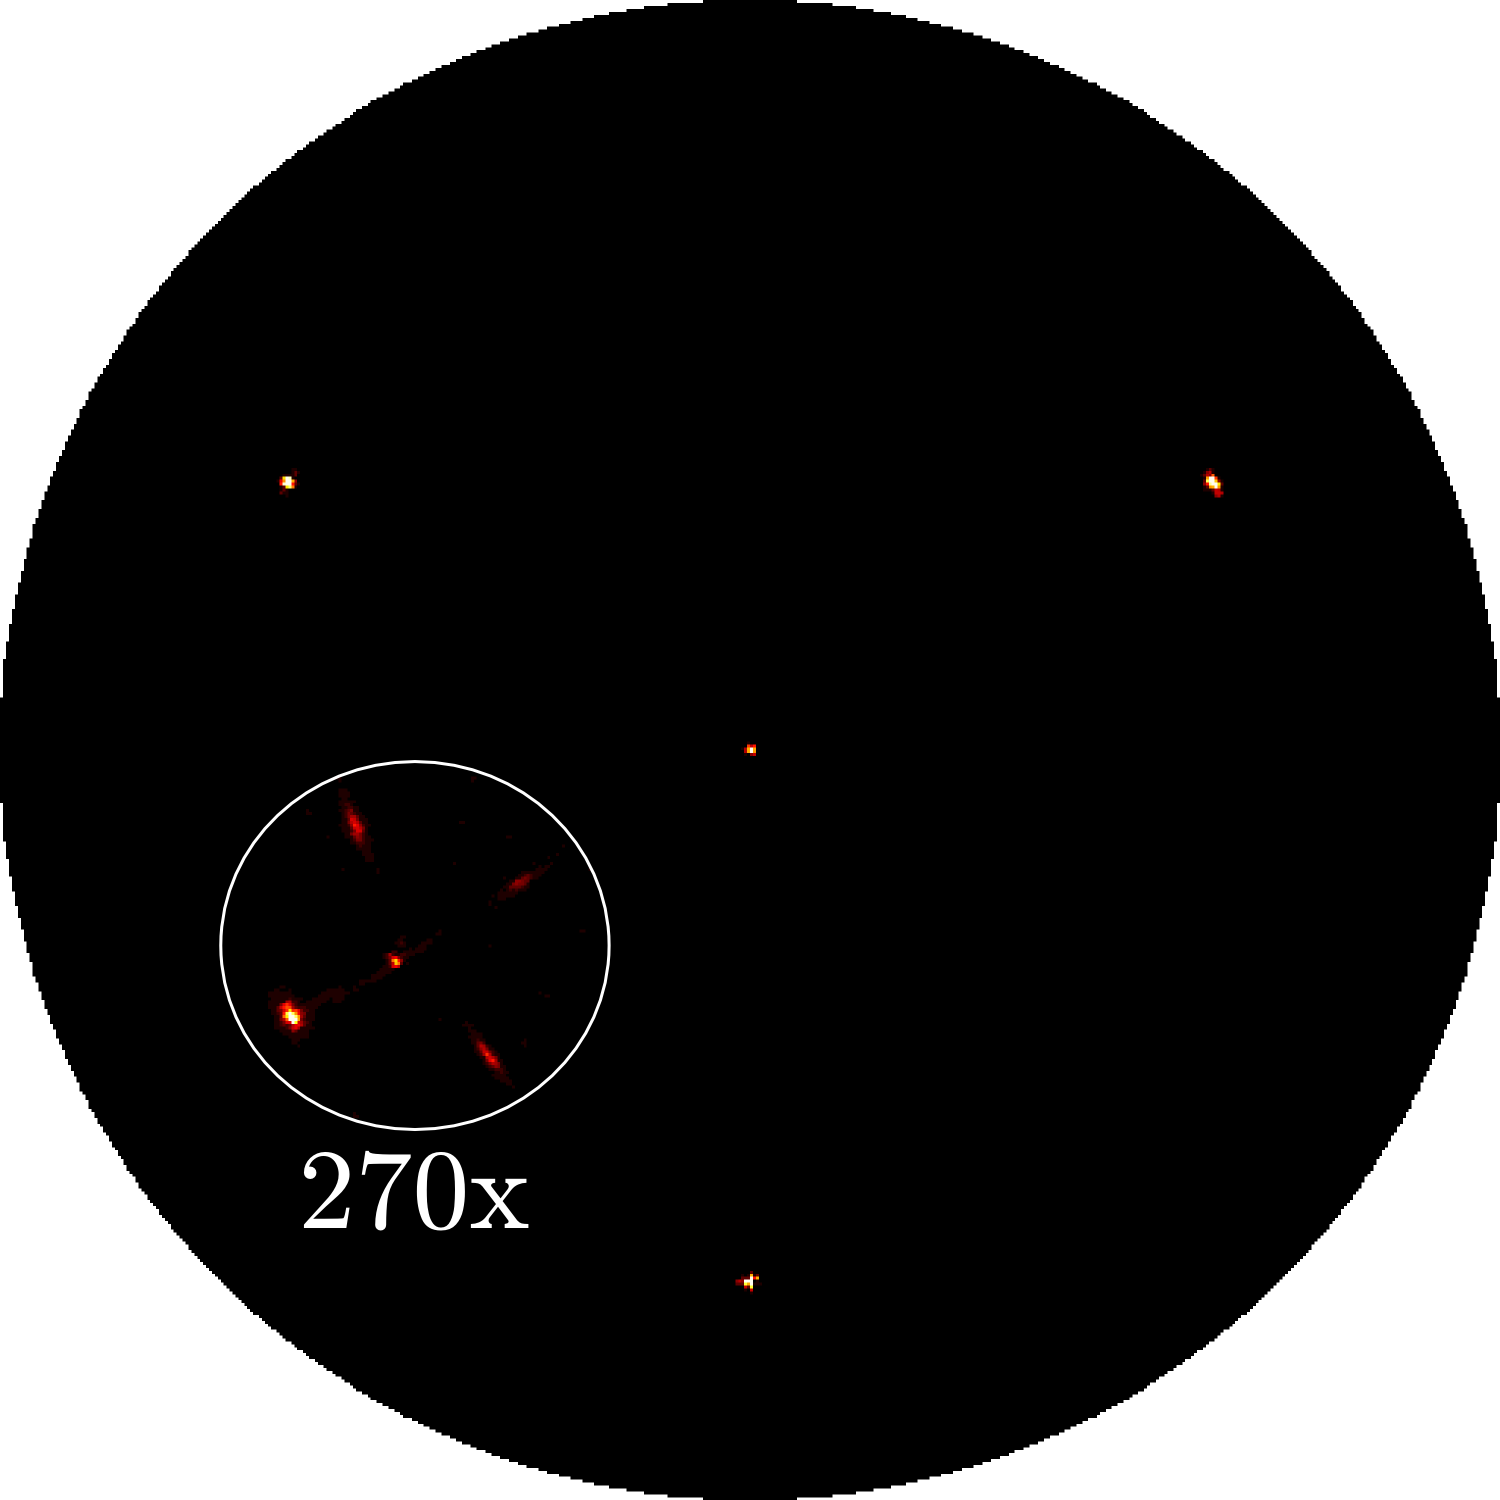
\includegraphics[width=\textwidth]{cdteliftoff_F22_attached}
        \caption{\label{fig:cdteliftoff_F22_attached}(111) Pole figure of as-grown CdTe on sapphire}
    \end{subfigure} %
    \begin{subfigure}[b]{0.4\textwidth}
        \centering
        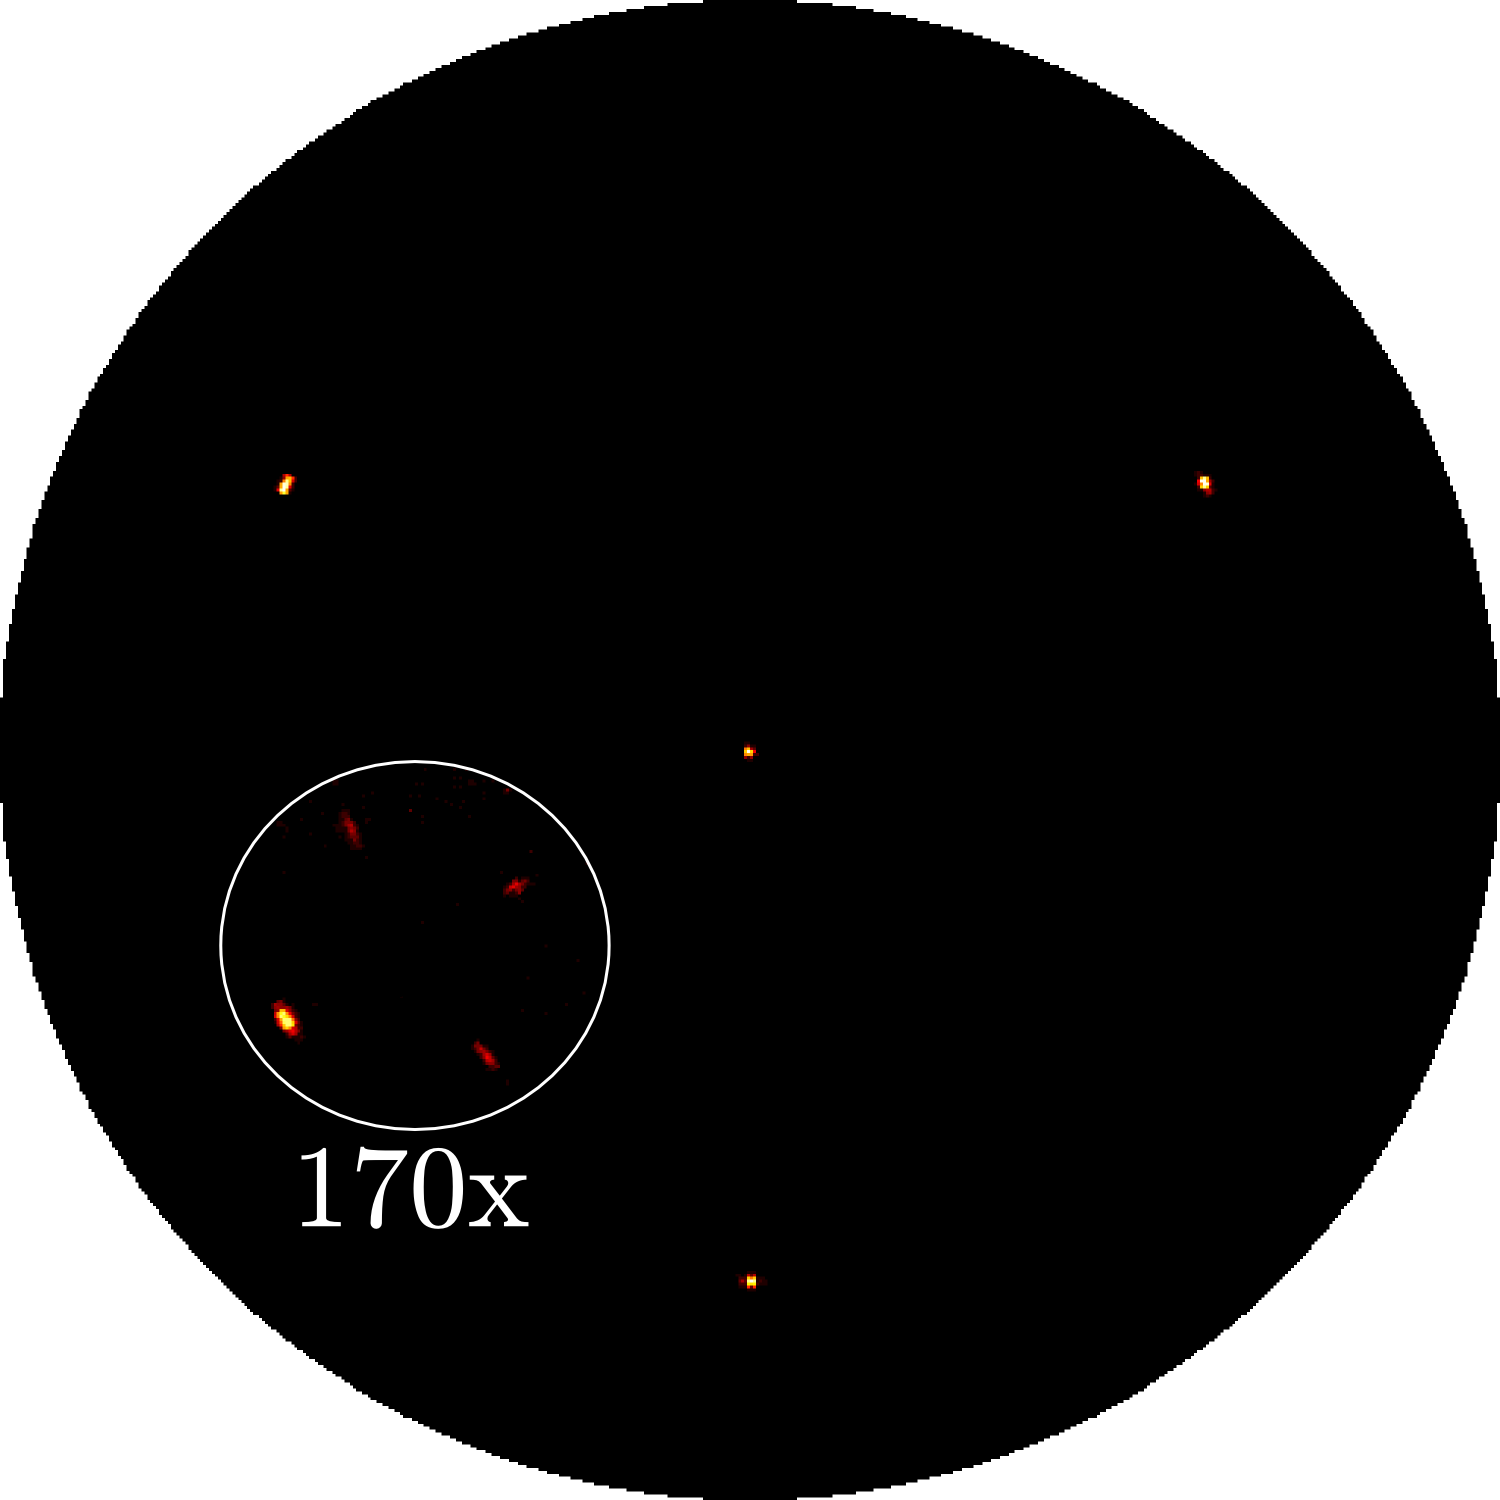
\includegraphics[width=\textwidth]{cdteliftoff_F22_released}
        \caption{\label{fig:cdteliftoff_F22_released}2DXRD of single crysal CdTe thin film on epoxy carrier}
    \end{subfigure}
    \caption{\label{fig:cdteliftoff_2DXRD}Attached and released CdTe pole figures}
\end{figure}



\section{Implications for Symmetry and Energy at Epitaxial Surfaces}

\chapter{CdTe Growth on Reconstructed SrTiO3}
%\section{Introduction}
As part of the ongoing research into the growth of CdTe, various other oxide single crystals were examined for possible use as substrates. One of those substrates, SrTiO\textsubscript{3}, while it did not ultimately yield particularly high quality CdTe, did provide some interesting insights into the potential for surface reconstructions to play a role in epitaxy.

The role of both substrate offcut and high temperature surface reconstructions were examined through the growth of CdTe on as-received and reconstructed SrTiO\textsubscript{3} substrates. This work was done in close collaboration with Dr. Robert Hughes and Dr. Svetlana Neretina and was published in Applied Surface Science\cite{Neretina2009a}.
\section{Experimental}
CdTe films were deposited on both the as-received and
reconstructed surface of (100) SrTiO\textsubscript{3} (MTI Corporation). Step-
terrace formation relied upon the miscut originating from the
inaccuracies in the crystallographic alignment carried out prior to
the cutting and polishing of the substrates (manufacturer’s miscut
tolerance 0.5\degree). As a result, the degree of miscut could only be
varied through the use of substrates from different batches. Due to
the high temperatures required, the surface reconstruction took
place ex situ in a quartz tube furnace. Prior to annealing, the
substrates were etched in BHF for 90~s. Anneals were conducted in
flowing oxygen (60 SCCM) at 1000\celsius{} for 10~h. \cref{fig:srtio3_sub_afm} shows
atomic force microscopy (AFM) images for the as-received and
surface reconstructed substrates relevant to this work. As
expected, only the annealed substrates exhibit the step-terrace
structure with unit cell step heights. The difference in terrace
width for the surfaces shown in \cref{fig:srtio3_sub_afm}b and c can be attributed to a
miscut difference estimated at 0.358\degree. Also present on each image
are the crystallographic axes obtained through X-ray diffraction
(XRD). Note that a nearly identical in-plane step direction exists for
both reconstructed surfaces. As this direction is close to, but not
aligned with the [011] axis of SrTiO\textsubscript{3}, it is expected that the steps
exhibit a sawtooth morphology, but on length scales not readily
observed using atomic force microscopy.
\begin{figure}
    \centering
    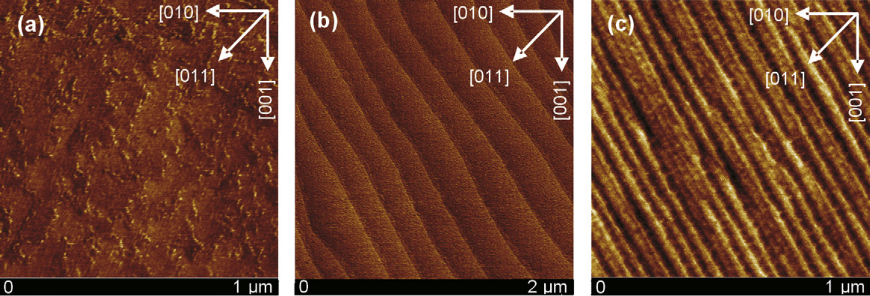
\includegraphics[width=\textwidth]{srtio3_sub_afm}
    \caption[AFM of SrTiO\textsubscript{3} surfaces]{\label{fig:srtio3_sub_afm}AFM images for the (a) as-received (100) SrTiO\textsubscript{3} substrate, (b) a reconstructed surface with an average terrace width of approximately 200 nm and (c) a reconstructed surface with a terrace width of approximately 50 nm. From the step heights and terrace widths it is estimated that the miscuts for the two reconstructed surfaces are (b) 0.118\degree{}
        and (c) 0.468\degree{}.}
\end{figure}

CdTe films were deposited on the three SrTiO\textsubscript{3} surfaces shown
in \cref{fig:srtio3_sub_afm} using pulsed laser deposition. A deposition rate of 20 nm/min was achieved by
operating the laser at a repetition rate of 10~Hz with a substrate to
target distance of 3.5~cm. Films were grown to
a thickness of 300~nm as determined using a spectroscopic variable
angle ellipsometer (Horiba Jobin Yvon, France). Morphological and
structural characterization was then conducted on the films
produced using AFM and 2DXRD.
\section{Results and Discussion}
\cref{fig:srtio3_pole} shows the (111) CdTe pole figures for the three substrates
shown in \cref{fig:srtio3_sub_afm}. The dramatic differences observed between films
deposited on the as-received and annealed substrates indicate that
the surface reconstruction gives rise to a complete re-alignment of
the CdTe grains. The pole figure for the as-received surface is
consistent with a [111] oriented film. The fact that twelve peaks
exist in the outer ring, instead of the three expected for a single
crystal, indicates that there are four in-plane grain orientations.
The pole figures for the films deposited on the surface reconstructed substrates show that both films are predominantly [211]
oriented. The twelve peaks in the central ring and twenty-four
peaks in the outer ring denote twelve in-plane grain orientations. Each peak in the central ring comes from a different grain, the intensity differences indicate that some grains form
preferentially over others. Note that of the twelve peaks both
the strongest and weakest is in-line with the miscut direction for
both of the reconstructed surfaces and that the degree of this
preferential orientation is stronger for the reconstructed surface
having the narrow terrace width. An examination of the low
intensity pole figure peaks (not visible in the figures), indicates that
some [111] CdTe grains exist in these nominally [211] films, but
at the 10\% level. While these [111] grains contribute to
the intensity at the centre of the pole, the response there is almost
entirely due to the (100) SrTiO\textsubscript{3} substrate.
\begin{figure}
    \centering
    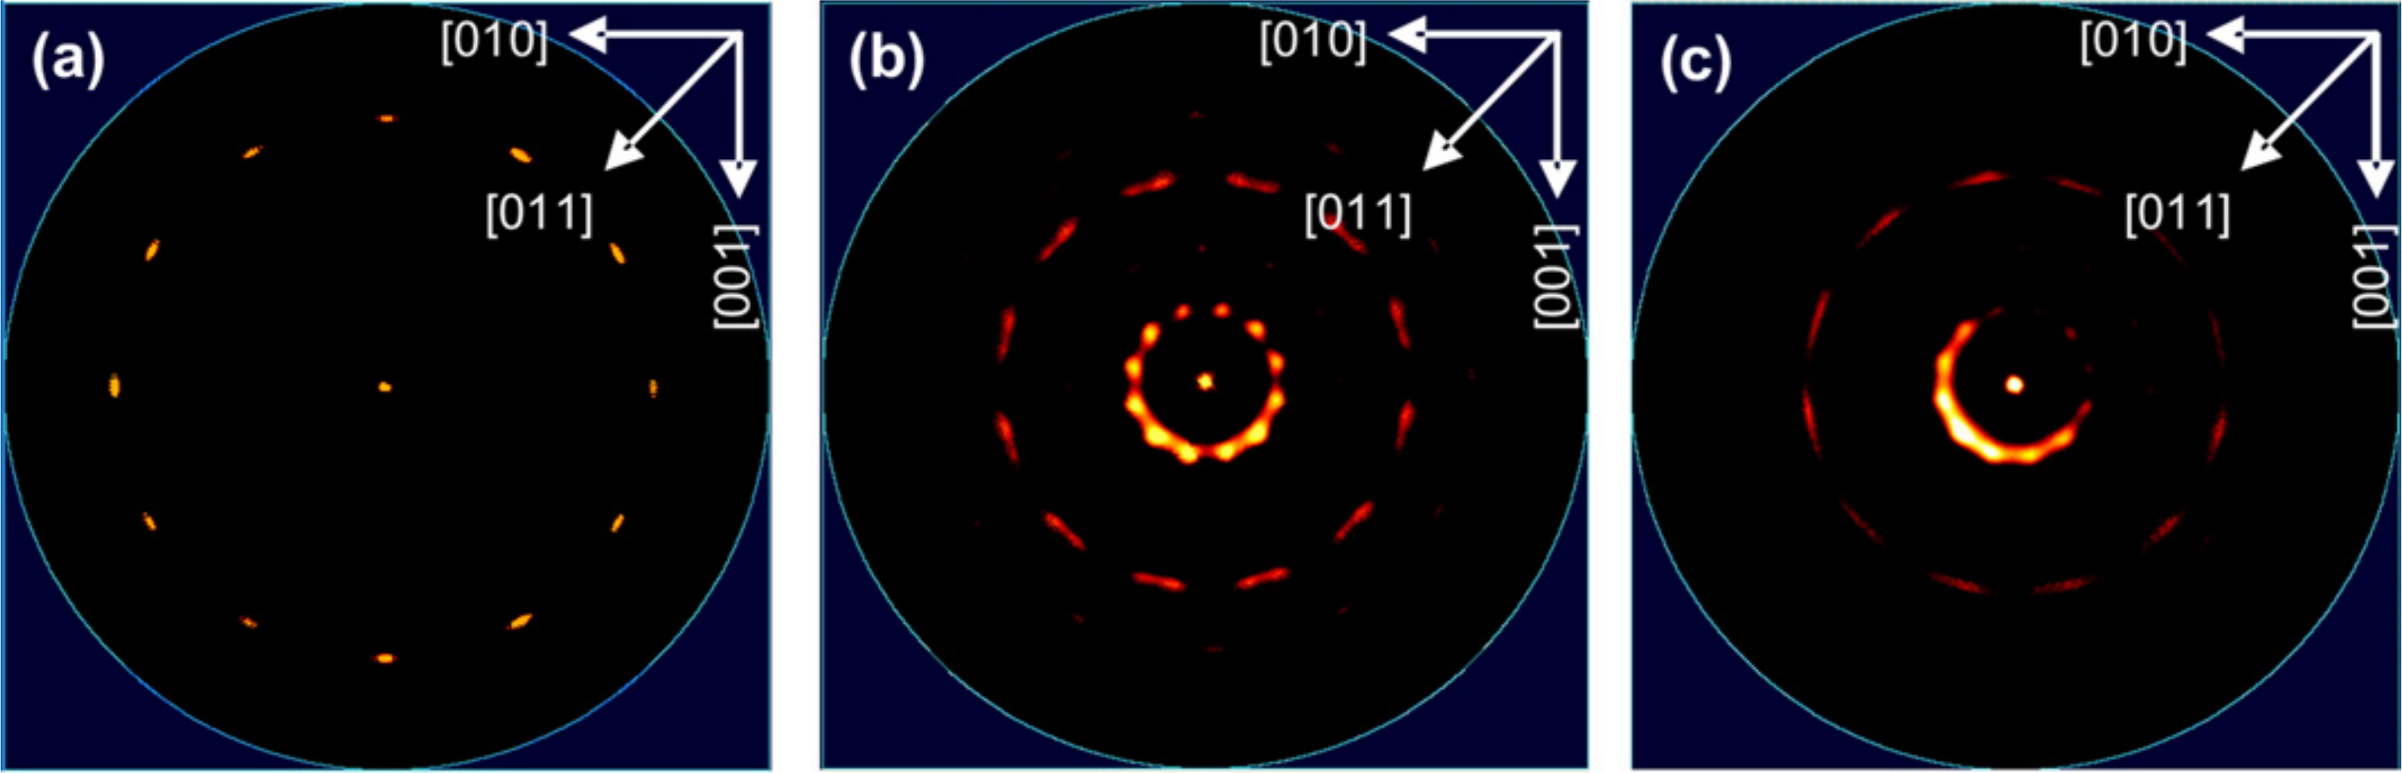
\includegraphics[width=\textwidth]{srtio3_pole}
    \caption[Pole figures of CdTe grown on SrTiO\textsubscript{3}]{\label{fig:srtio3_pole}(111) CdTe pole figures for films deposited on (a) the as-received (100) SrTiO\textsubscript{3} substrate (b) the reconstructed surface with wide terraces and (c) the reconstructed surface with narrow terraces. Indicated on each image are the substrate’s in-plane crystallographic axes obtained from XRD measurements.}
\end{figure}
\begin{figure}
    \centering
    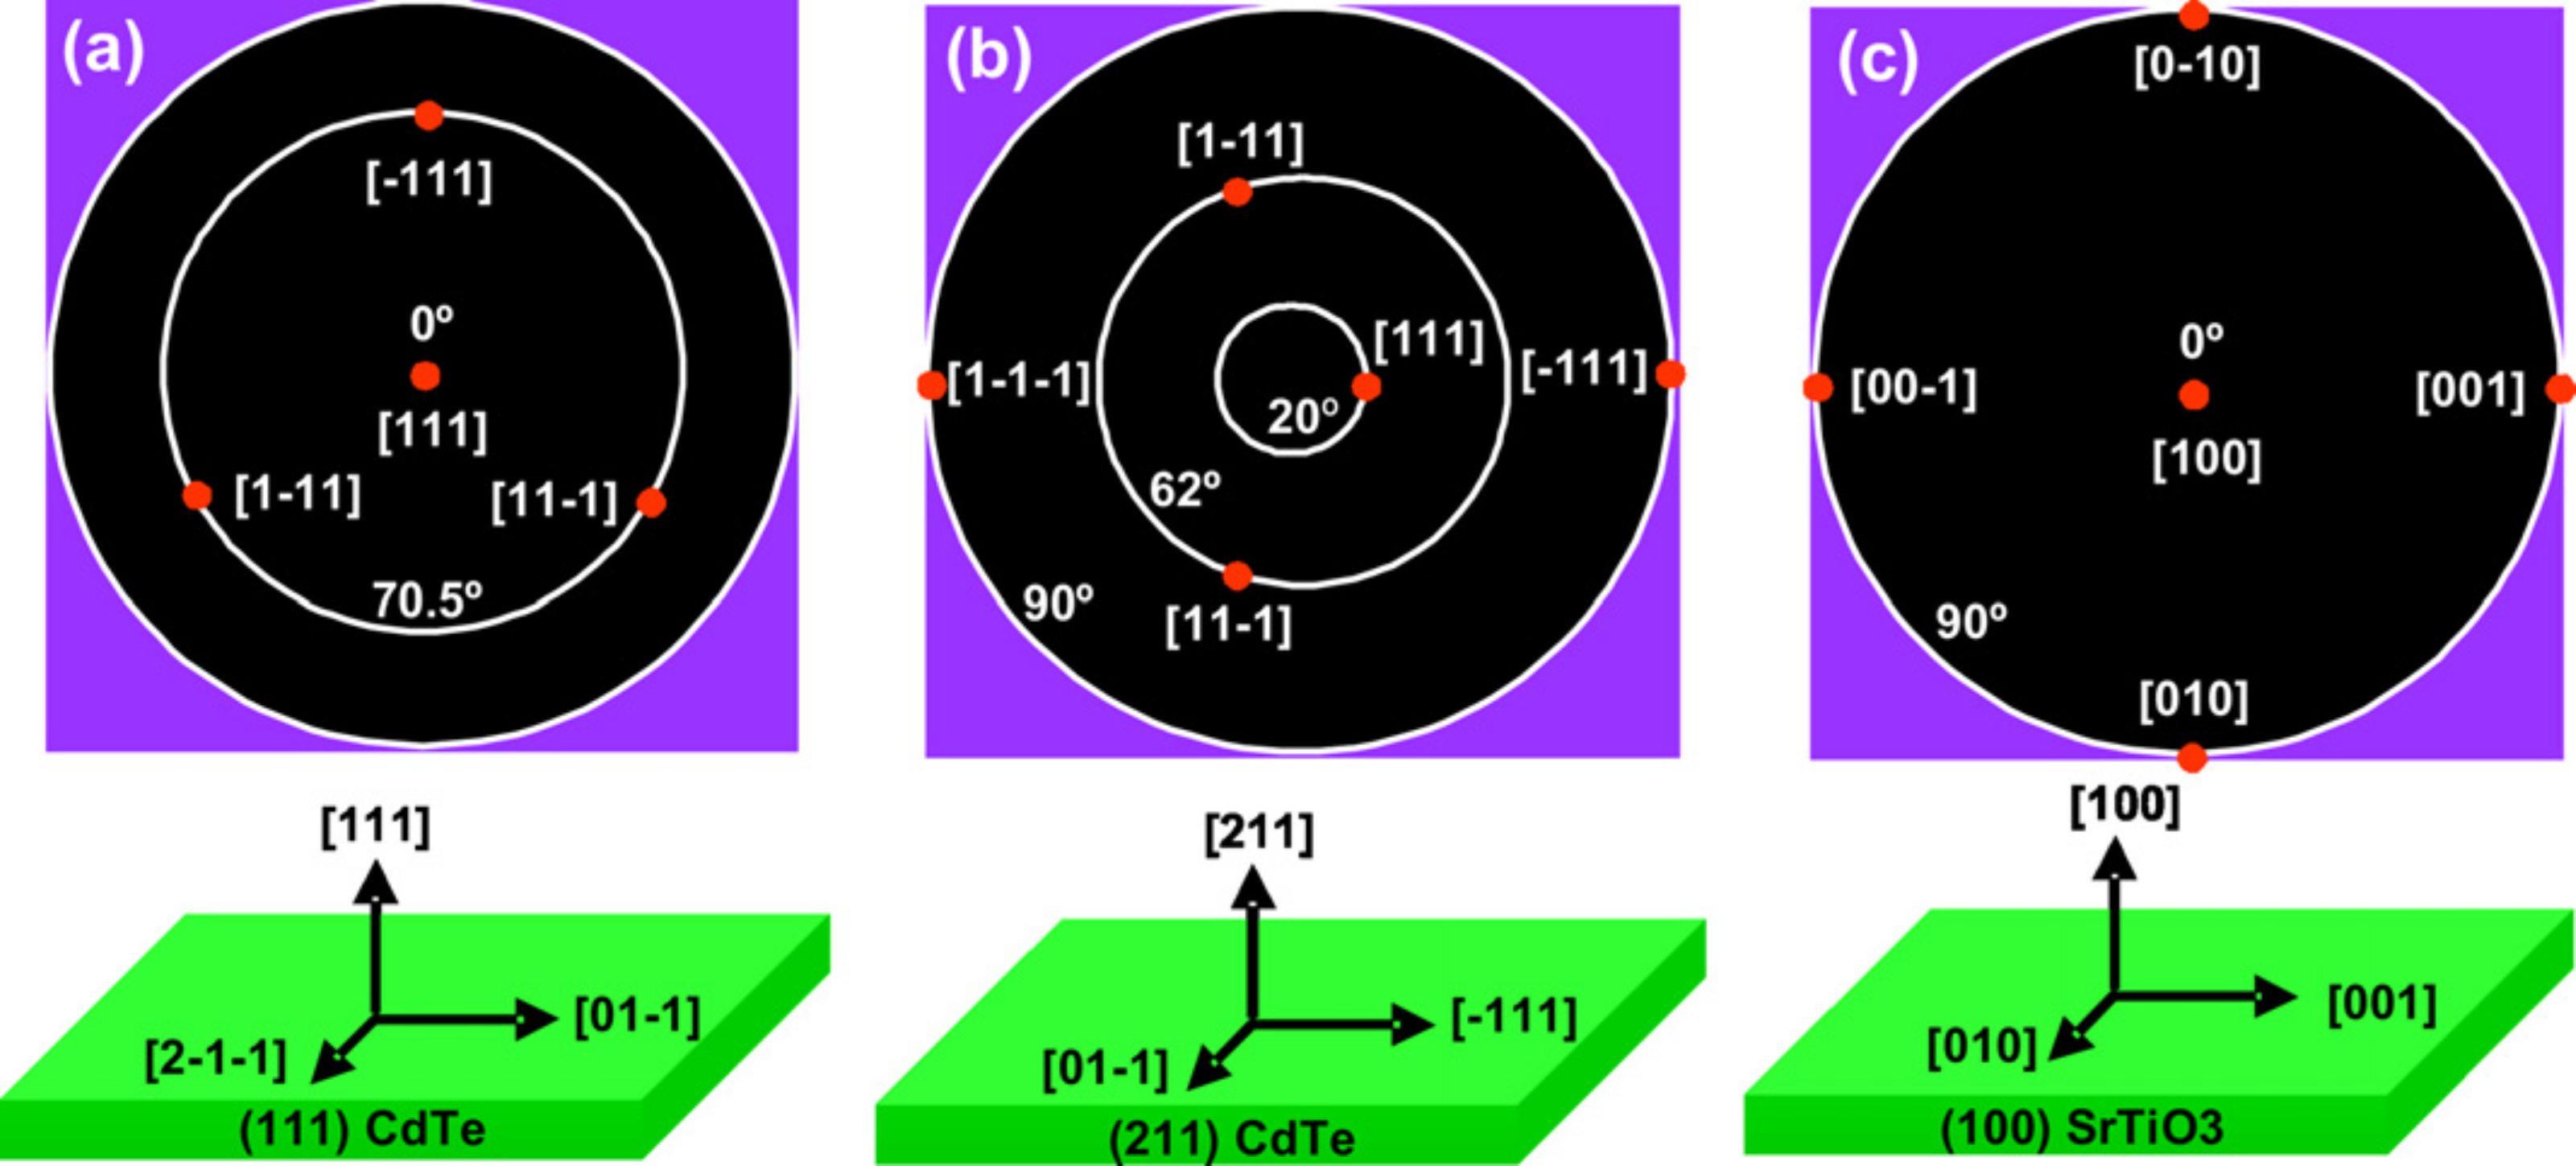
\includegraphics[width=\textwidth]{srtio3_sim_pole}
    \caption{\label{fig:srtio3_sim_pole}Schematics showing the (111) pole figure expected for a single crystal CdTe film with a a) [111] and b) [211] orientation. c) Schematic showing the (100) pole figure expected for a [100] oriented SrTiO\textsubscript{3} substrate. The surface normal and in-plane Miller indicies are also shown for each case.}
\end{figure}

Grain formation for a given film/substrate combination is
determined by the interface energy. For the case of the as-received
(100) SrTiO\textsubscript{3} substrate the interface energy is minimized through
the formation of [111] CdTe grains. This interfacial relationship is
not surprising as CdTe has demonstrated a high propensity for
forming it almost irrespective of the substrate surface offered\cite{Neretina2006}.
The resulting interface, however, must overcome the seemingly
incompatible situation brought about when the four-fold symmetric substrate surface mates with the six-fold symmetric (111)
plane of CdTe. In this scenario it is reasonable to expect that the
resulting in-plane grain structure reflects both a suitable fit to the
substrate’s atomic arrangement as well as its underlying symmetry. The (111) pole figure results indicate that this is indeed the
case as there exists a four-fold symmetric grain structure which is
commensurate with the substrate’s cubic crystal structure. The
XRD data indicates that these grains are oriented as shown
schematically in \cref{fig:srtio3_tri_on_100}a. The triangles symbolize the orientation of
the (111) planes on the surface of SrTiO\textsubscript{3} represented by the
dotted pattern. The arrows on the triangles denote the three
equivalent (111) CdTe planes that project out of its surface. Note
that each of these four triangles match poorly to the substrate’s
lattice constant in all but one direction. In this direction, it is nearly
equal to two of the substrate’s unit cells (mismatch = 1.6\%). This
one-dimensional match is preferred to such extents that only
grains that comply with it exist within the film. To appreciate the
uniqueness of the four grains it should be noted that, for the arrows
denoting the (111) equivalent planes, no two arrows point in the
same direction. It is these directions that give rise to the twelve
peaks in the outer ring of the (111) pole figure as is evident from
\cref{fig:srtio3_tri_on_100}b.
\begin{figure}
    \centering
    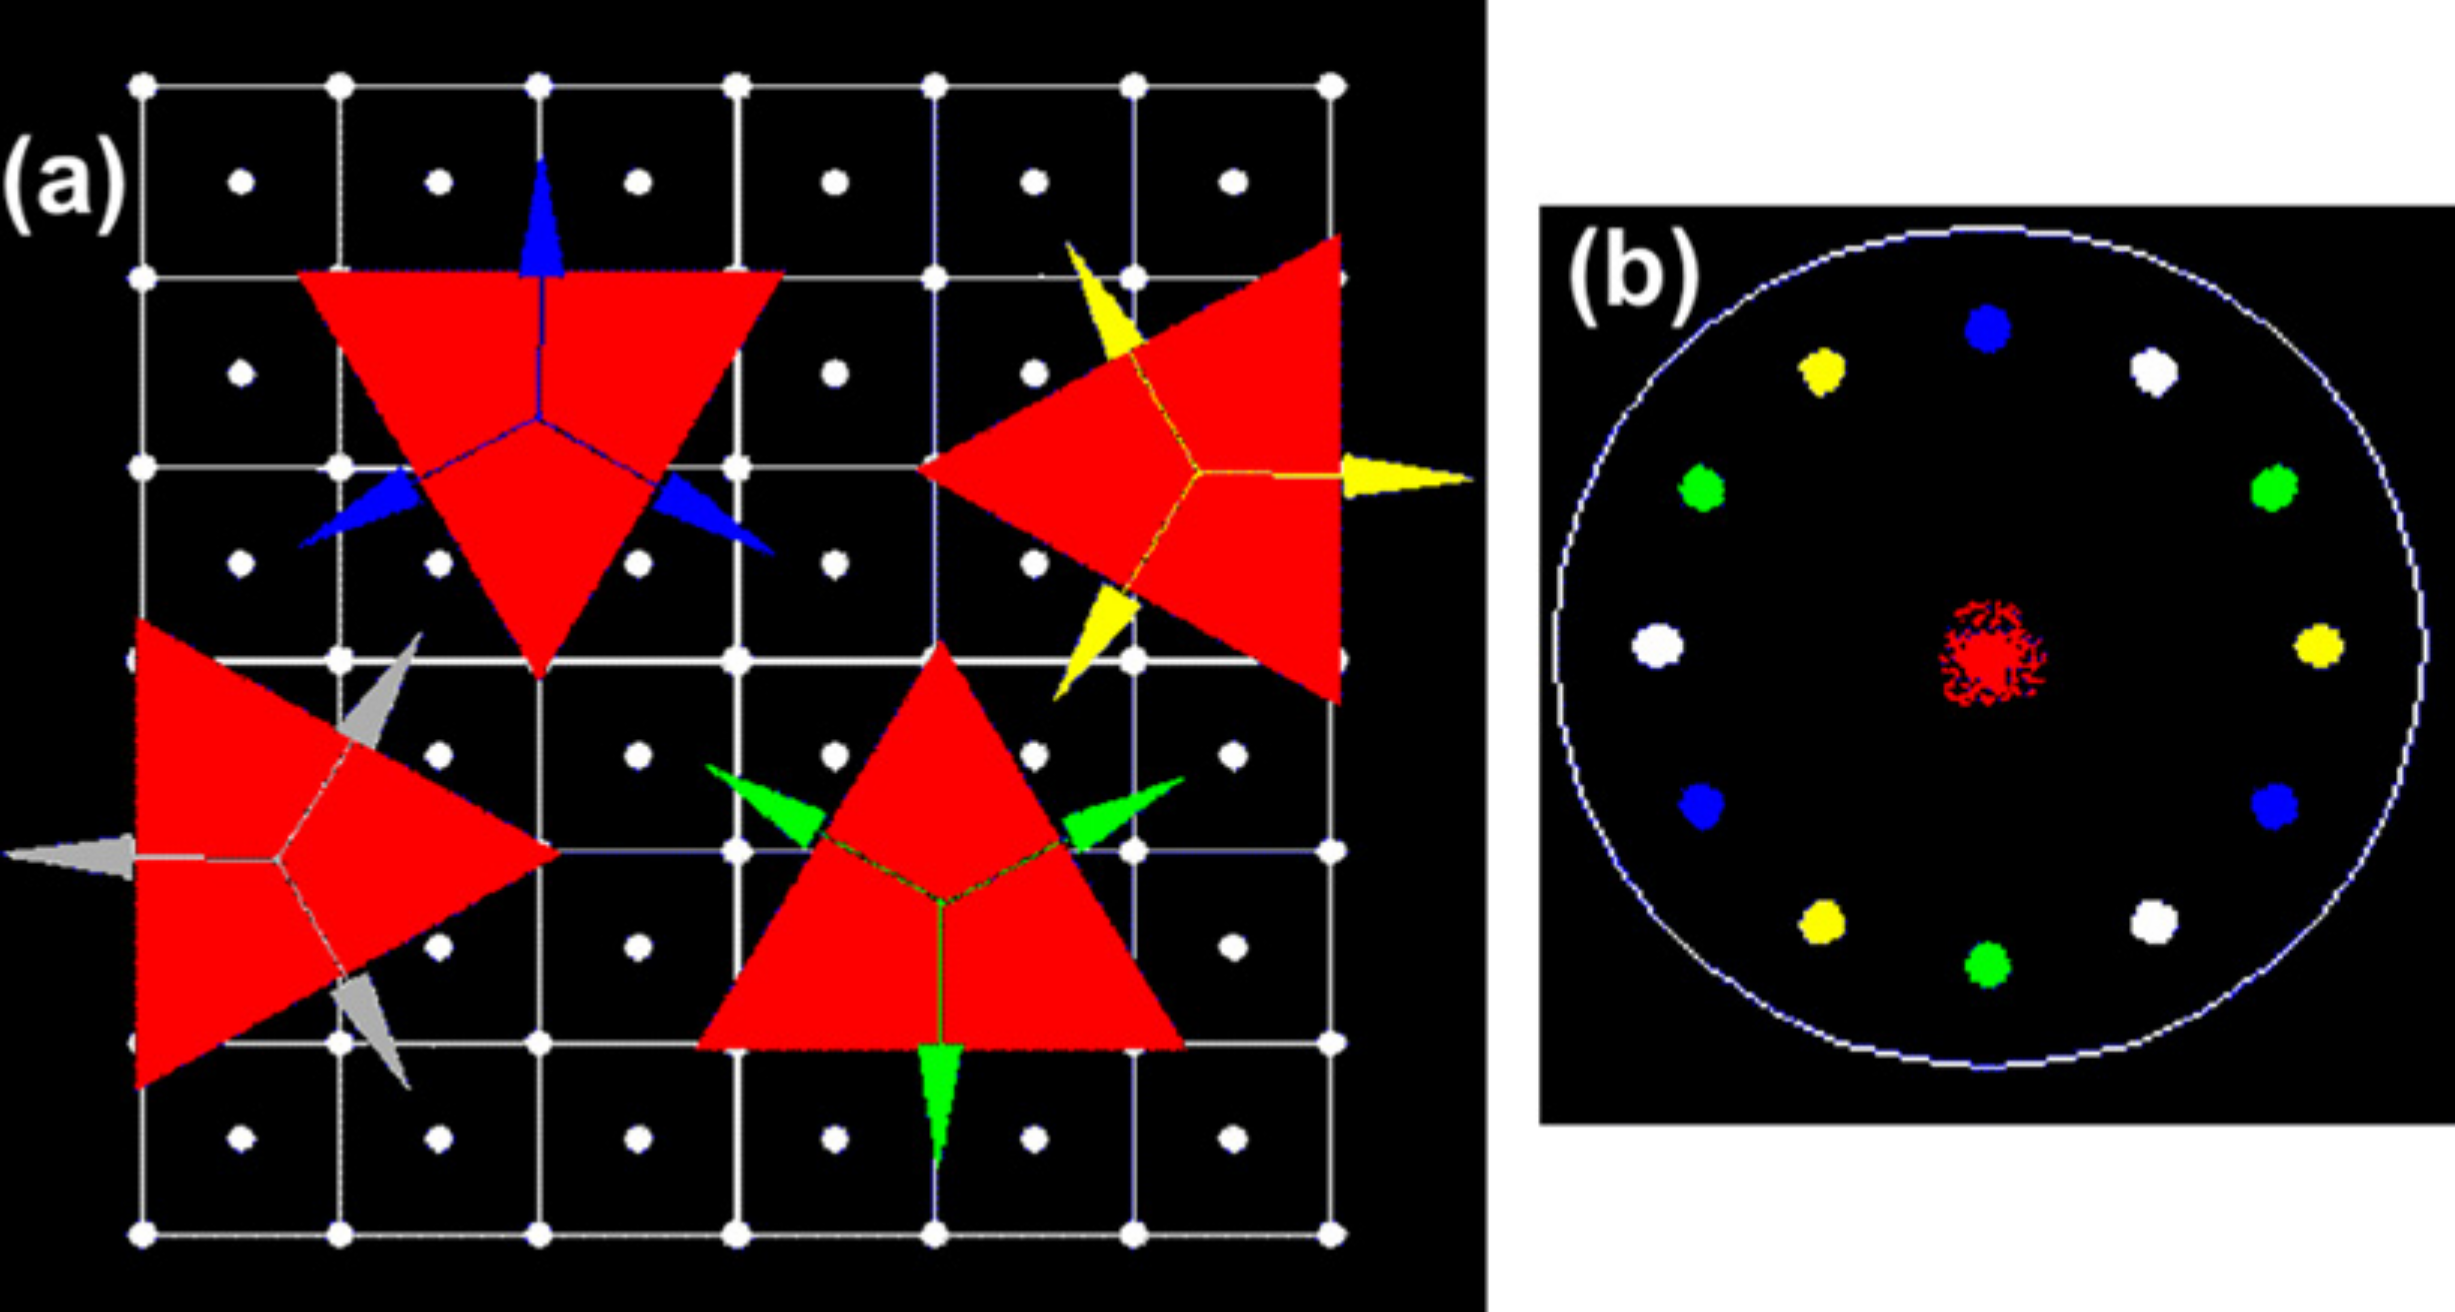
\includegraphics{srtio3_tri_on_100}
    \caption[CdTe grains on (100) SrTiO\textsubscript{3}]{\label{fig:srtio3_tri_on_100}a) Schematic illustrating the four possible [111] CdTe grain orientations (triangles) for films deposited on the SrTiO\textsubscript{3} substrate (dotted background). The arrows on
        each triangle denote the direction of the three equivalent (111) planes that emerge from the surface. Note that no two arrows are pointing in the same direction. For each
        grain orientation there exists a one-dimensional geometrical fit (mismatch = 1.6\%) to the substrate in either the vertical or horizontal directions. b) Schematic showing the
        resulting (111) pole figure obtained from the four grains where the colour of the dot on the pole figure corresponds to the grain from which it was derived.}
\end{figure}
\begin{figure}
    \centering
    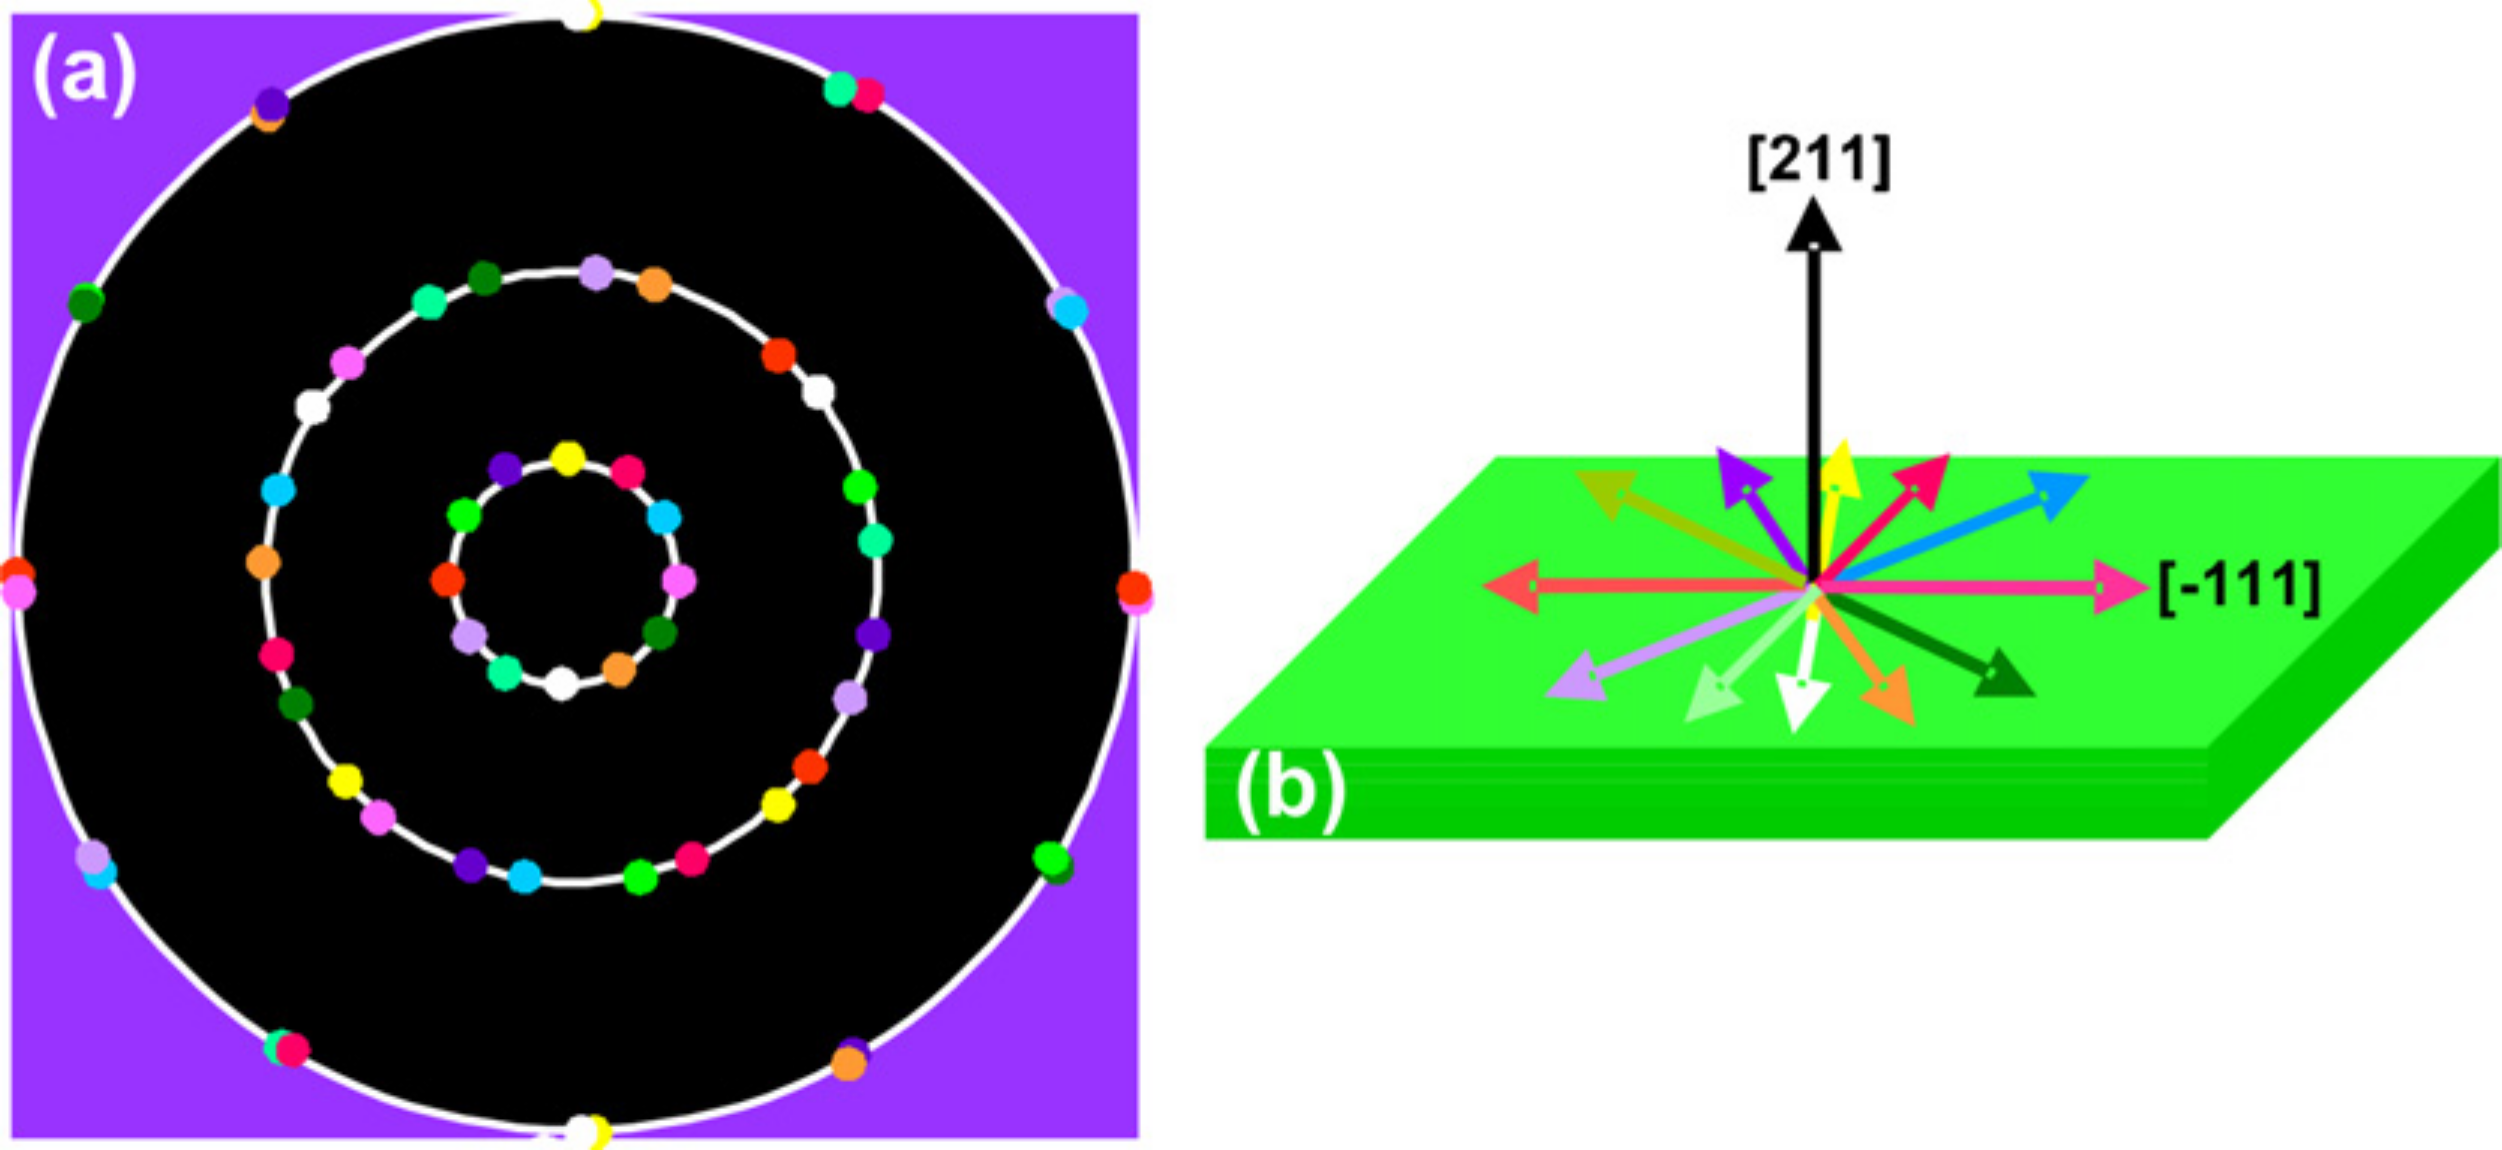
\includegraphics{srtio3_211_sim_polefigure}
    \caption[Simulated pole figure of CdTe on reconstructed SrTiO\textsubscript{3}]{\label{fig:srtio3_211_sim_polefigure}a) Schematic detailing the twelve-fold symmetric [211] CdTe grain structure observed for films deposited on the surface reconstructed substrates. The contribution
        from each grain is denoted by a different colour. Note that the pattern corresponding to a single crystal [211] CdTe film (\cref{fig:srtio3_sim_pole}b) is repeated twelve times. b) Schematic showing the in-plane [$\overline{1}$11] direction for each of the [211] grains.}
\end{figure}

The formation of a [211] CdTe film on a surface reconstructed
(100) SrTiO\textsubscript{3} substrate was quite unexpected. CdTe films with this
orientation have been deposited, but only when the interface
energy is minimized through the use of [211] oriented substrates
\cite{Lange1991b,Million1996,Rujirawat1997a,Zanatta1998}. While [211] substrates provide an appropriate template
for [211] growth, there exist no obvious symmetry arguments
that would allow for twelve symmetrically distributed grains to be
accommodated on the bulk surface of (100) SrTiO\textsubscript{3}. Instead, it is
expected that the origin of the [211] CdTe grains lies with the
epitaxial relationship formed between the (211) planes and the
surface reconstruction. In this case, it is expected that the twelve-fold symmetric grain structure is commensurate with the underlying symmetry of the substrate’s surface reconstruction. Thus,
insight into the nature of the reconstruction is obtained from the
observed grain structure. \Cref{fig:srtio3_211_sim_polefigure} shows a schematic representation
of the (111) CdTe pole figure where the contributions from each
grain are shown. The pole figure’s inner ring demonstrates a
twelve-fold symmetry in the grain structure as it is comprised of twelve nearly equally spaced peaks where each peak originates
from a different grain orientation. Also of significance is the fact
that the wide terrace widths shown in \cref{fig:srtio3_sub_afm}b give rise to [211]
CdTe grains even though the film grain size is often smaller than
the width of the terrace. Thus, it appears that [211] grain
formation does not rely on nucleation at the substrate steps. This is
a strong indication that the atomic scale surface reconstruction is a
dominant factor in the promotion of the [211] grains.

Of the three surface reconstructions known to form in an
oxygen ambient, only the c($4\times2$) and c($6\times2$) reconstructions
present a surface structure where there exist reasonable symmetry
arguments able to account for the formation of a [211] CdTe film
having a twelve-fold symmetric grain structure. Such a grain
structure must arise from the symmetries of the underlying
substrate as it provides the only means for the isolated grains to
establish a symmetrical arrangement when first formed in an
island growth mode. The (211) plane of CdTe, shown in \cref{fig:srtio3_cdte211}, is
one-fold symmetric and consists of a series of rows comprised of
alternating cadmium and tellurium atoms separated by distances of 8.49 or 2.83 \AA. \Cref{fig:srtio3_c4x2} shows a schematic of the c($4\times2$) TiO\textsubscript{2} surface reconstruction proposed by Castell\cite{Castell2002}. It consists of a
series of alternating rows of titanium and oxygen atoms. The top
layer has a TiO\textsubscript{2} stoichiometry, but it is sparsely populated with
only one quarter the number of atoms present in the TiO\textsubscript{2} layers
found in the bulk\cite{Castell2002}. With every second row of titanium atoms
offset relative to each other they align in a pseudo-six-fold
symmetric pattern. Possible geometric fits of the (211) CdTe plane
to this surface reconstruction are shown in \cref{fig:srtio3_c4x2}b. Each of the three
possible geometric fits shown would give rise to two unique grain
types due to the one-fold symmetry of the (211) plane. Six other
domain structures would also form by virtue of the fact that the
c($4\times2$) surface reconstruction has two possible domains rotated
90\degree~relative to each other\cite{Castell2002}. The domain structure that develops
on the reconstructed surface arises from the fact that the rows of
titanium atoms have an equal probability of forming along the
[010] or [001] directions. The net result would be a twelve-fold
symmetric [211] CdTe grain structure. The c($6\times2$) surface
reconstruction, proposed by Jiang and Zegenhagen\cite{Jiang1996}, is shown
schematically in \cref{fig:srtio3_cdte211}. It too is a sparsely populated surface that
has the potential to accommodate the (211) CdTe planes in select
directions (\cref{fig:srtio3_cdte211}b). Here, the four geometrical fits shown give rise
to eight unique grain types. In a manner analogous to the c($4\times2$)
reconstruction, the c($6\times2$) reconstruction also has a domain
structure that gives rise to an additional set of eight grains rotated
90\degree{} to the ones shown in the figure. An examination of these
additional grains, however, reveals that only four of them provide
unique solutions as the other four rotate into solutions offered by
the first domain. Thus, a twelve-fold ($8 + 8 \times 4 = 12$) symmetric
(211) CdTe grain structure is expected for this surface.
\begin{figure}
    \centering
    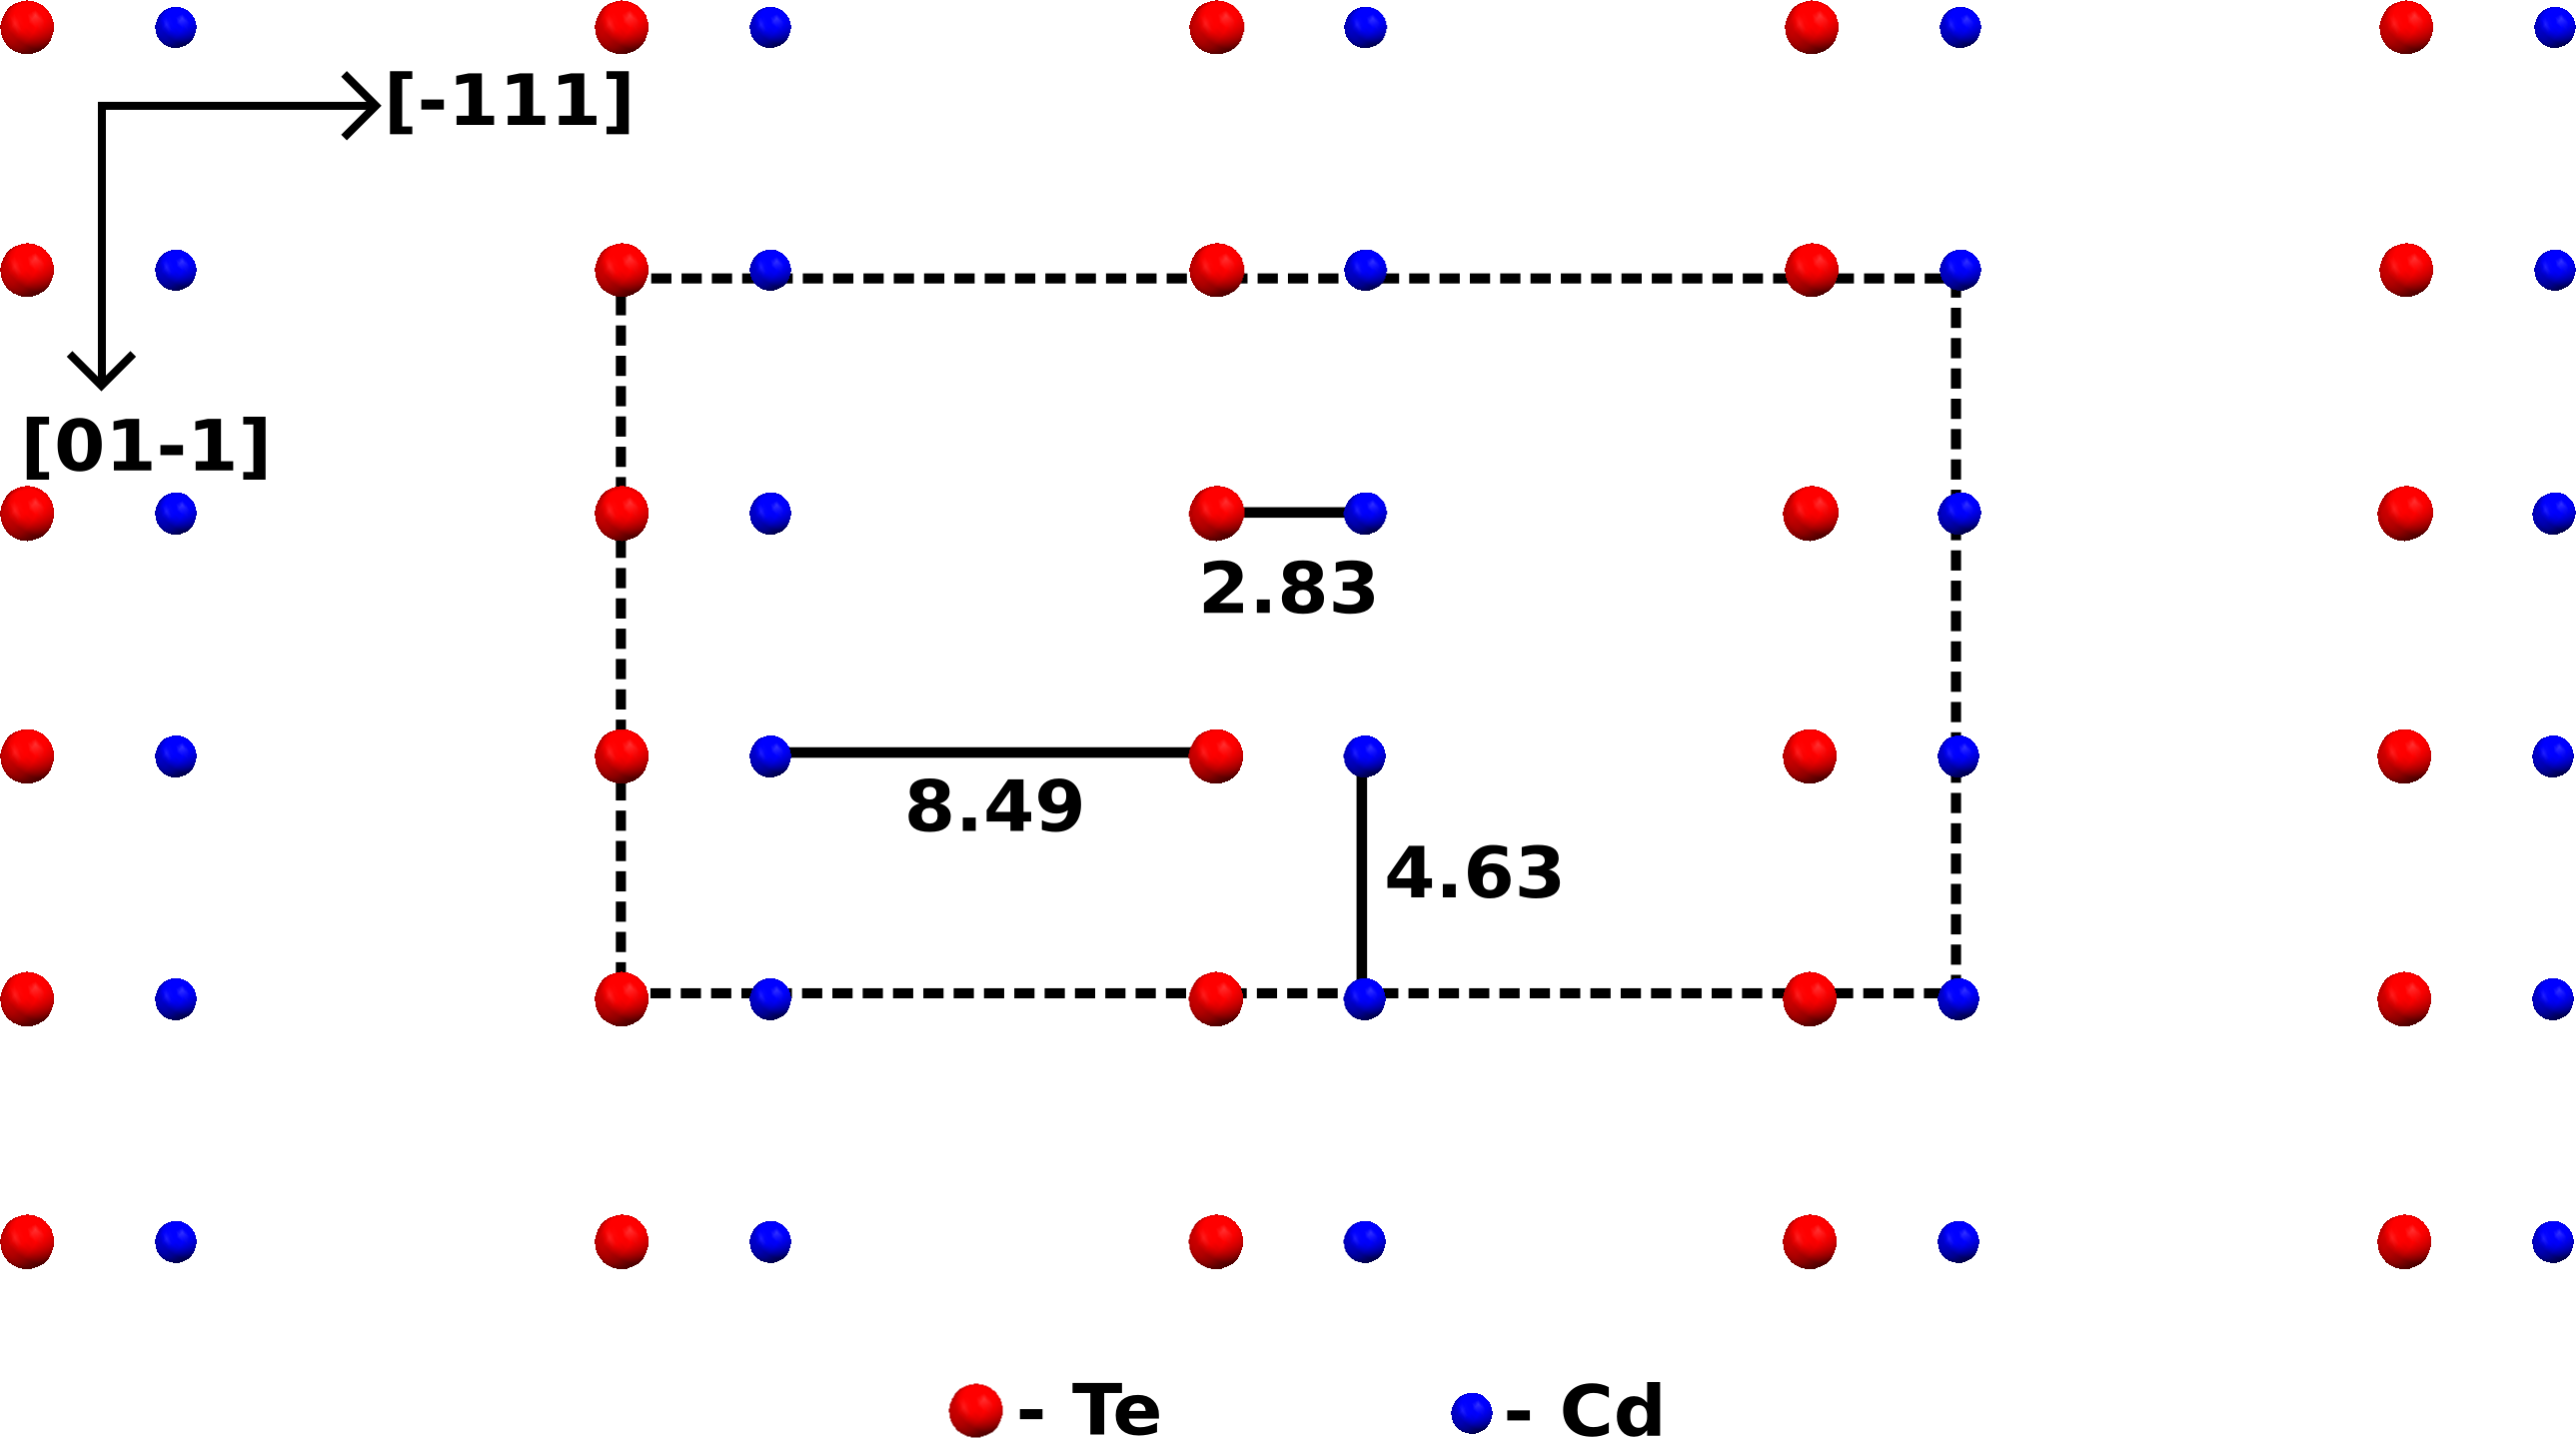
\includegraphics[width=0.8\textwidth]{srtio3_cdte211}
    \caption[Projection of (211) CdTe unit cell on SrTiO\textsubscript{3} surface]{\label{fig:srtio3_cdte211}Schematic of the (211) plane of CdTe with the interplanar dimensions
        labelled in units of angstroms. The area outlined by the dashed lines is used in
        subsequent figures to demonstrate how this structure fits to (100) SrTiO\textsubscript{3} surface
        reconstructions. The Miller indices shown correspond to the crystallographic
        orientation of the (211) CdTe plane.}
\end{figure}
\begin{figure}
    \centering
    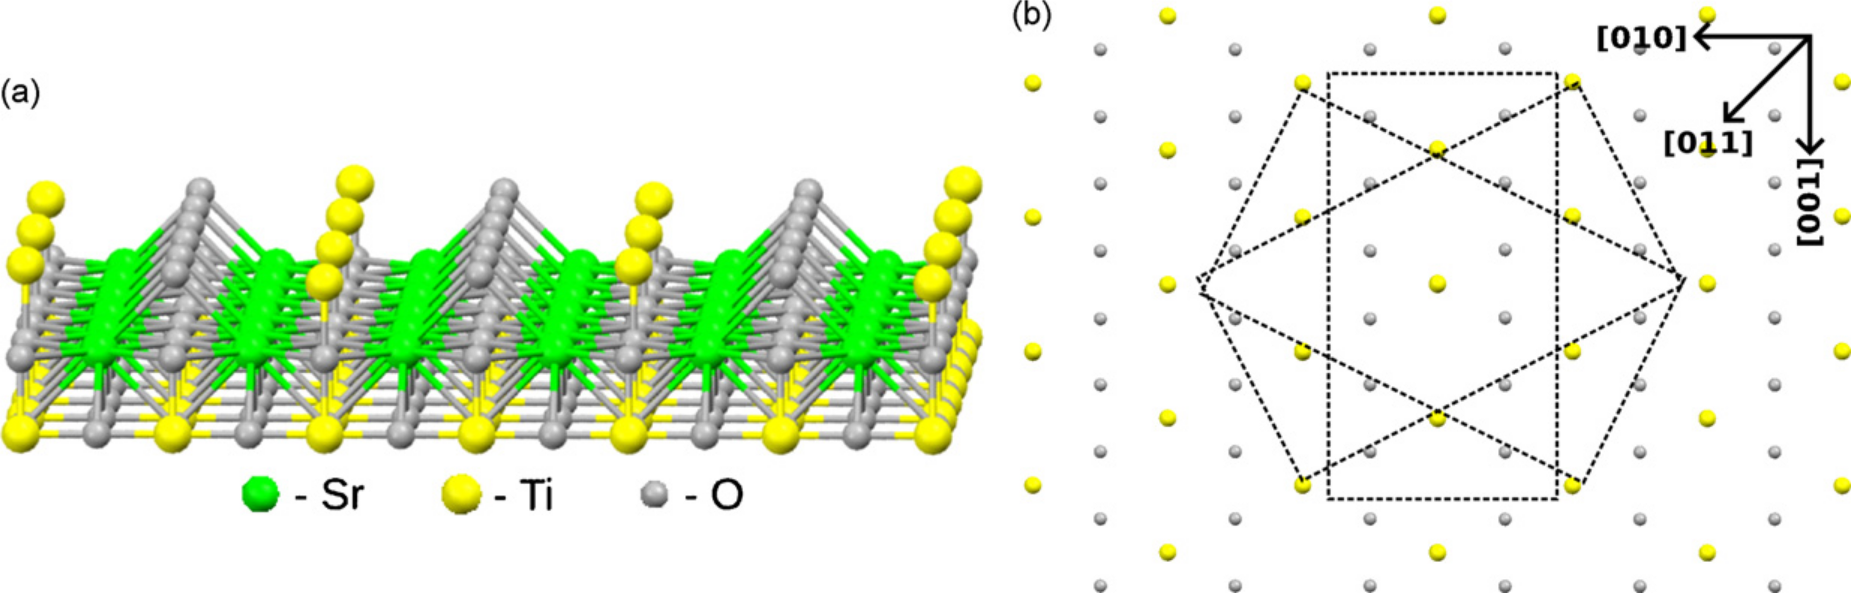
\includegraphics[width=\textwidth]{srtio3_c4x2}
    \caption[CdTe on c(4$\times$2) SrTiO\textsubscript{3} surface]{\label{fig:srtio3_c4x2}(a) Schematic showing the surface of the (100) SrTiO\textsubscript{3} with a c($4\times2$) surface reconstruction. (b) Schematic showing the uppermost layer of the reconstruction with the dashed lines being used to illustrate the closest geometrical fits of the (211) CdTe plane to this surface. The three orientations shown give rise to six grain orientations as a 180\degree~rotation of the (211) plane yields a different grain structure. This is a consequence of the fact that the single crystal (111) CdTe pole figure for a [211] film is one-fold symmetric (see \cref{fig:srtio3_sim_pole}b). Six other grain structures arise from a domain structure in the substrate surface reconstruction that would be schematically represented by a 90\degree{} rotation of \cref{fig:srtio3_c4x2}b. The Miller indices shown in the top right corner of the figure correspond to the crystallographic orientation of the underlying bulk (100) SrTiO\textsubscript{3} substrate.}
\end{figure}

Assuming that the orientation relationships between CdTe
and the surface reconstructions shown in \cref{fig:srtio3_c4x2,fig:srtio3_c6x2} are adhered
to then it becomes possible to experimentally predict the surface
reconstruction undergone by the substrates presented in this
work. It should be noted from \cref{fig:srtio3_c4x2}b that the c($4\times2$)
reconstruction is characterized by (211) CdTe grain alignment
along the substrate’s [010] and [001] directions. \Cref{fig:srtio3_pole}b
shows that this is not the case, ruling out this reconstruction for the
work presented here. It does not, however, rule out the possibility
of [211] CdTe grain growth if a film were deposited on such a
reconstruction. The c($6\times2$) reconstruction, on the other hand,
requires grain growth along the substrate’s [011] and [0$\overline{1}$1]
directions, consistent with the X-ray data. While we have no direct
evidence that the c($6\times2$) surface reconstruction formed, it is of
note that the anneal conditions used elsewhere\cite{Jiang1996} to obtain this
reconstruction are similar to those used here. While it should be
understood that predicting a film-substrate orientation relationship solely on the basis of a geometrical fit is somewhat na\"{\i}ve, it is well established that this scenario occurs more often than not.
\begin{figure}
    \centering
    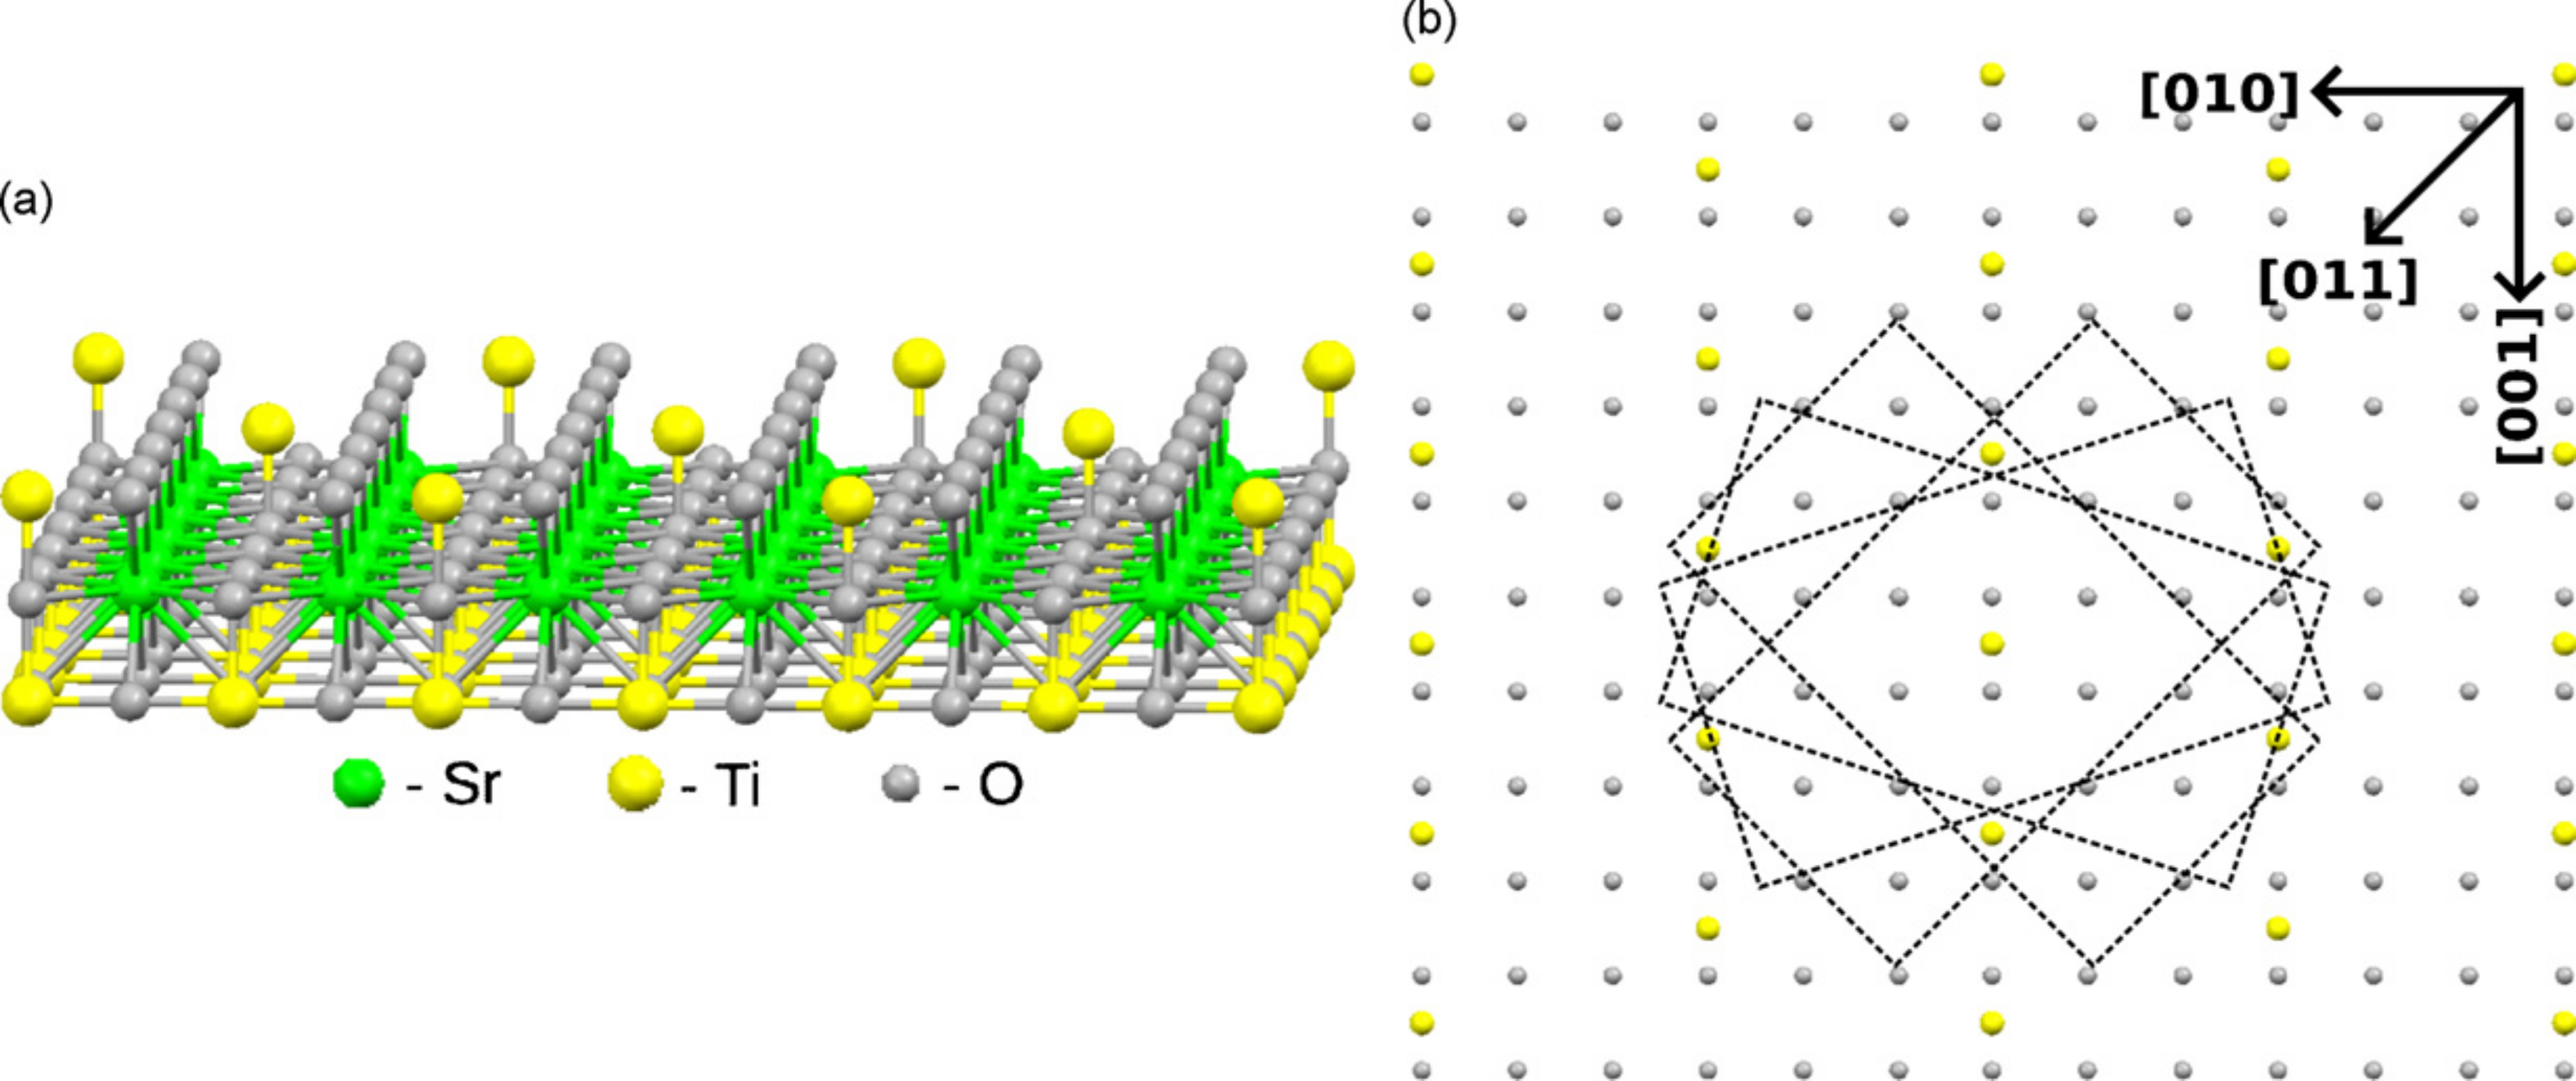
\includegraphics[width=\textwidth]{srtio3_c6x2}
    \caption[CdTe on c(6$\times$2) SrTiO\textsubscript{3} surface]{\label{fig:srtio3_c6x2}(a) Schematic showing the surface of the (100) SrTiO\textsubscript{3} with a c($6\times2$) surface reconstruction. (b) Schematic showing the uppermost layer of the reconstruction with the
        dashed lines being used to illustrate the closest geometrical fits of the (211) CdTe plane to this surface. The four orientations shown give rise to eight grain orientations as a
        180\degree{} rotation of the (211) plane yields a different grain structure. Eight other grain structures arise from a domain structure in the substrate surface reconstruction that
        would be schematically represented by a 90\degree~rotation of \cref{fig:srtio3_c4x2}b. Of these eight grains only four represent unique solutions as the grains forming along the [011] and [01$\overline{1}$]
        directions rotate into each other. The Miller indices shown in the top right corner of the figure correspond to the crystallographic orientation of the underlying bulk (100)
        SrTiO\textsubscript{3} substrate.}
\end{figure}

Even though both the [211] oriented films show pole figure
peaks in similar positions, the relative intensities of the peaks are
quite different. This is most easily seen by examining the
innermost ring of the pole figure where each of the twelve peaks
corresponds to a unique grain orientation. For both samples the
peaks on one side of the ring show greater intensities than on the
other. This effect, however, is much more pronounced for the pole
figure shown in \cref{fig:srtio3_pole}c. Here, the ratio of the integrated intensities
between the largest and smallest peak in the ring is 22 compared to
4 for the pole figure shown in \cref{fig:srtio3_pole}b. The fact that the terrace
width is approximately four times smaller for the film that shows
the most pole figure anisotropy suggests that the step edges
promote this preferential grain alignment. Consistent with this
explanation is the fact that the highest intensity peaks correspond
to the CdTe grain orientation having its [111] in-plane direction
normal to the step. The larger grain sizes exhibited by the surface
with smaller terraces are also expected within this scenario. This is
a simple consequence of the fact that, in the early stages of film
growth, there are more similarly oriented grains that are able to
merge into a single larger grain as is expected for an island growth
mechanism. With a sizeable effect being observed between the two
reconstructed surfaces having a miscut difference of only 0.358, the
potential exists to amplify this effect using a substrate with a
significantly larger miscut.

The results presented here demonstrate that the reconstructed
surface of (100) SrTiO\textsubscript{3} profoundly alters the grain structure of
CdTe films. While it is not unusual for the grain structure to be
transformed by the presence of a step-terrace morphology, it is
unprecedented for SrTiO\textsubscript{3}’s atomic-scale reconstructions to pro-
mote a film with an alternative heteroepitaxial relationship. For
the case of (100) SrTiO\textsubscript{3}, there seems to be a disconnect between
the research advocating a step-flow growth mode and the wide
array of atomic-scale surface reconstructions allowed, with the
latter not considered as a determining factor in the film quality
achieved. This may be due to the relatively high growth
temperatures used in the fabrication of oxide thin films. In this
case, the thermal energy available likely facilitates a local
rearrangement of surface atoms in response to the addition of
adatoms. This is certainly the case for the homoepitaxial growth of
silicon where the surface reconstruction gives way to bulk
crystalline ordering for temperatures in excess of 300\celsius{}\cite{Gossmann1985}.
For the low growth temperatures used in the fabrication of these
CdTe films the surface reconstruction is likely locked in place,
forcing CdTe to accommodate itself on the reconstructed surface.
The sparsely populated nature of such a surface should make it
prone to alternative epitaxial relationships as the interface would
not consist of an abrupt boundary, but instead, of an amalgamation
of two interpenetrating layers. Consistent with this explanation is
the fact that different (100) SrTiO\textsubscript{3} surface reconstructions give
rise to palladium nanodots having variable orientations and
faceting\cite{Silly2005b}.
\section{Implications for Symmetry and Energy at Epitaxial Surfaces}
While the results presented here don't explicitly improve the growth of the CdTe thin films, they do add to the understanding of the role of the interface in epitaxy. In all the cases presented here, the substrate used for epitaxial growth has a nominal orientation of (100), with very small miscut of less than 1\degree. Despite a fixed orientation for the substrate, the thin surface net presented to the epitaxial thin film dominates the nucleation and growth orientation. These results show that it is possible to leverage high temperature surface reconstructions in order to completely transform a given substrate. If a reconstruction can be created at high temperature and then locked-in at the growth temperature substrates that don't immediately appear to be an epitaxial match can end up presenting an ideal template for growth. The additional symmetry breaking that is available for offcut substrates can widen the range of acceptable substrates, by triggering a step-flow growth mode suppressing unwanted orientations.

For this type of surface net epitaxy to yield the most benefit, surface science research must investigate the zoo of surface reconstructions possible on the commercially available complex oxides. Many of the higher element complex oxides (YAG, YSZ, GGG etc.) have little to no literature examining their surface reconstructions or their behaviour when miscut. Phase diagrams of such surfaces would be highly beneficial in predicting good matches for epitaxy.
\chapter{CdTe Nanowire Growth on Sapphire}
%\section{Introduction}

\section{Background}

\section{Experimental}
The experimental results and procedures presented here will
focus on those nanowires derived from Bi\textsubscript{2}Te\textsubscript{3} catalytic seeds
deposited on pristine (0001) sapphire substrates. The results
obtained will then be compared to the CdTe nanowires,
described elsewhere [19], obtained using bismuth catalytic
seeds deposited on alcohol-altered (0001) sapphire substrates.The experimental results and procedures presented here will
focus on those nanowires derived from Bi\textsubscript{2}Te\textsubscript{3} catalytic seeds
deposited on pristine (0001) sapphire substrates. The results
obtained will then be compared to the CdTe nanowires,
described elsewhere [19], obtained using bismuth catalytic
seeds deposited on alcohol-altered (0001) sapphire substrates.

The Bi\textsubscript{2}Te\textsubscript{3} seeds were prepared using the PLD process
(GSI Lumonics IPEX-848 excimer laser, \textlambda~= 248 nm, laser
energy density = 2 J cm\textsuperscript{-2} , laser spot size = 1.2$\times$1.2 mm\textsuperscript{2}).
The target used was prepared in-house from commercially
available Bi\textsubscript{2}Te\textsubscript{3} pieces (99.999\% purity). These pieces were
melted in a cylindrical graphite mould that was machined to
sizes able to yield a 1 inch target weighing approximately 10 g. This procedure was carried out in an argon background gas. Prior to the deposition, the sapphire substrate was heated to 
400\degree\celsius and held there for 10 min in an oxygen background 
pressure of 300 mTorr.The substrate was then cooled to room temperature where a 20 \AA thick film of Bi\textsubscript{2}Te\textsubscript{3} was deposited. This deposition lasted 35 s at a laser repetition rate of 3 Hz. 
Once deposited, the film was then heated to 370\degree\celsius where, over 
the course of 10 min, it would dewet forming Bi\textsubscript{2}Te\textsubscript{3} 
seeds. At this point, a 30 sccm helium flow was introduced 
into the chamber such that the pressure was maintained at 
400 mTorr. Material from a rotating CdTe target, grown using 
the Bridgman method, was then ablated onto the substrate for 
time intervals typically in the range of 30?45 min at a laser 
repetition rate of 8 Hz. The nanowires were then allowed to 
cool to room temperature in the helium ambient.

\section{Results and Discussion}
Figure 1 shows an SEM image, of the Bi\textsubscript{2}Te\textsubscript{3}
catalytic seeds formed on the (0001) sapphire substrate. The
seeds show a substantial size distribution with diameters
as large as 150 nm. While these seeds show enhanced
stability, they are still prone to evaporation and will disappear
completely if the CdTe deposition is delayed by approximately
10 min. As was the case for the bismuth catalysts, the Bi\textsubscript{2}Te\textsubscript{3}
seeds gain stability from exposure to the cadmium/tellurium
flux. It is also likely that the seeds shown in the image
are somewhat different from those available when nanowire
growth commences as the time required to cool these seeds
to room temperature provided ample opportunity for further
evaporation and Ostwald ripening.
\begin{figure}
    \centering
    \begin{subfigure}[t]{0.5\textwidth}
        \centering
        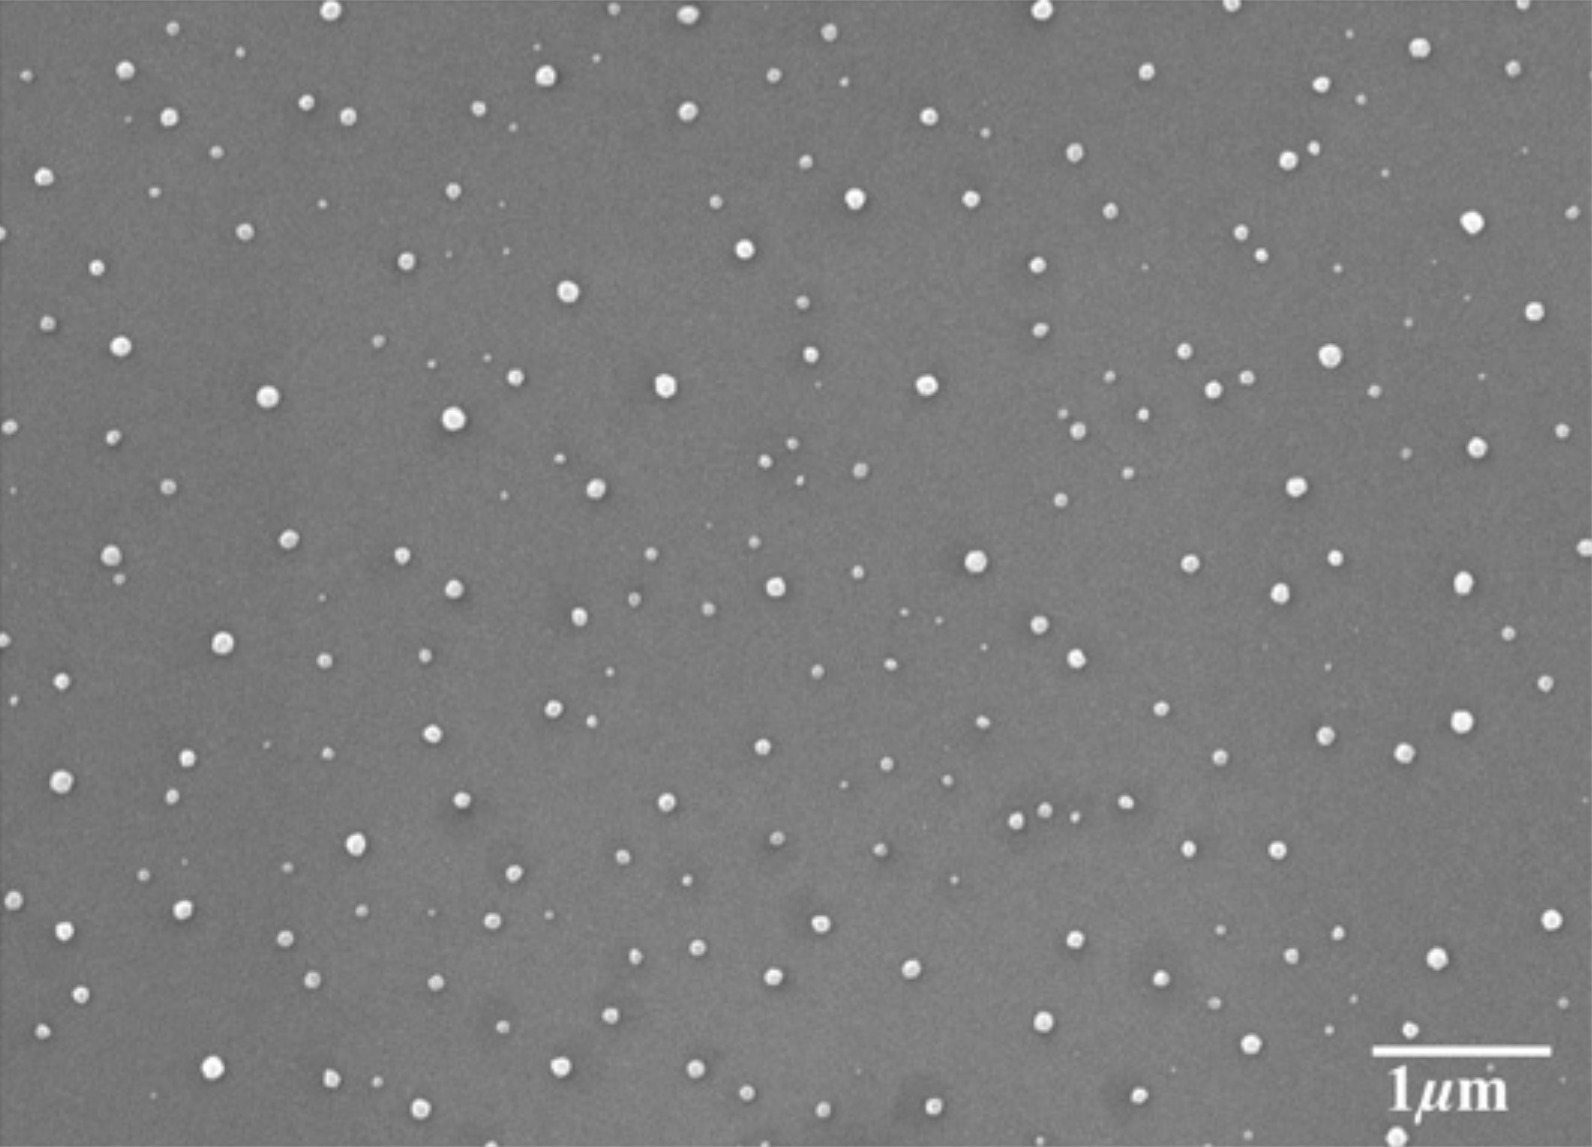
\includegraphics{nanocdte_bite}
        \caption{\label{fig:nanocdte_bite}SEM image of the Bi2 Te3 seeds that were used as catalysts 
            for CdTe nanowires.}
    \end{subfigure}%
    \begin{subfigure}[t]{0.5\textwidth}
        \centering
        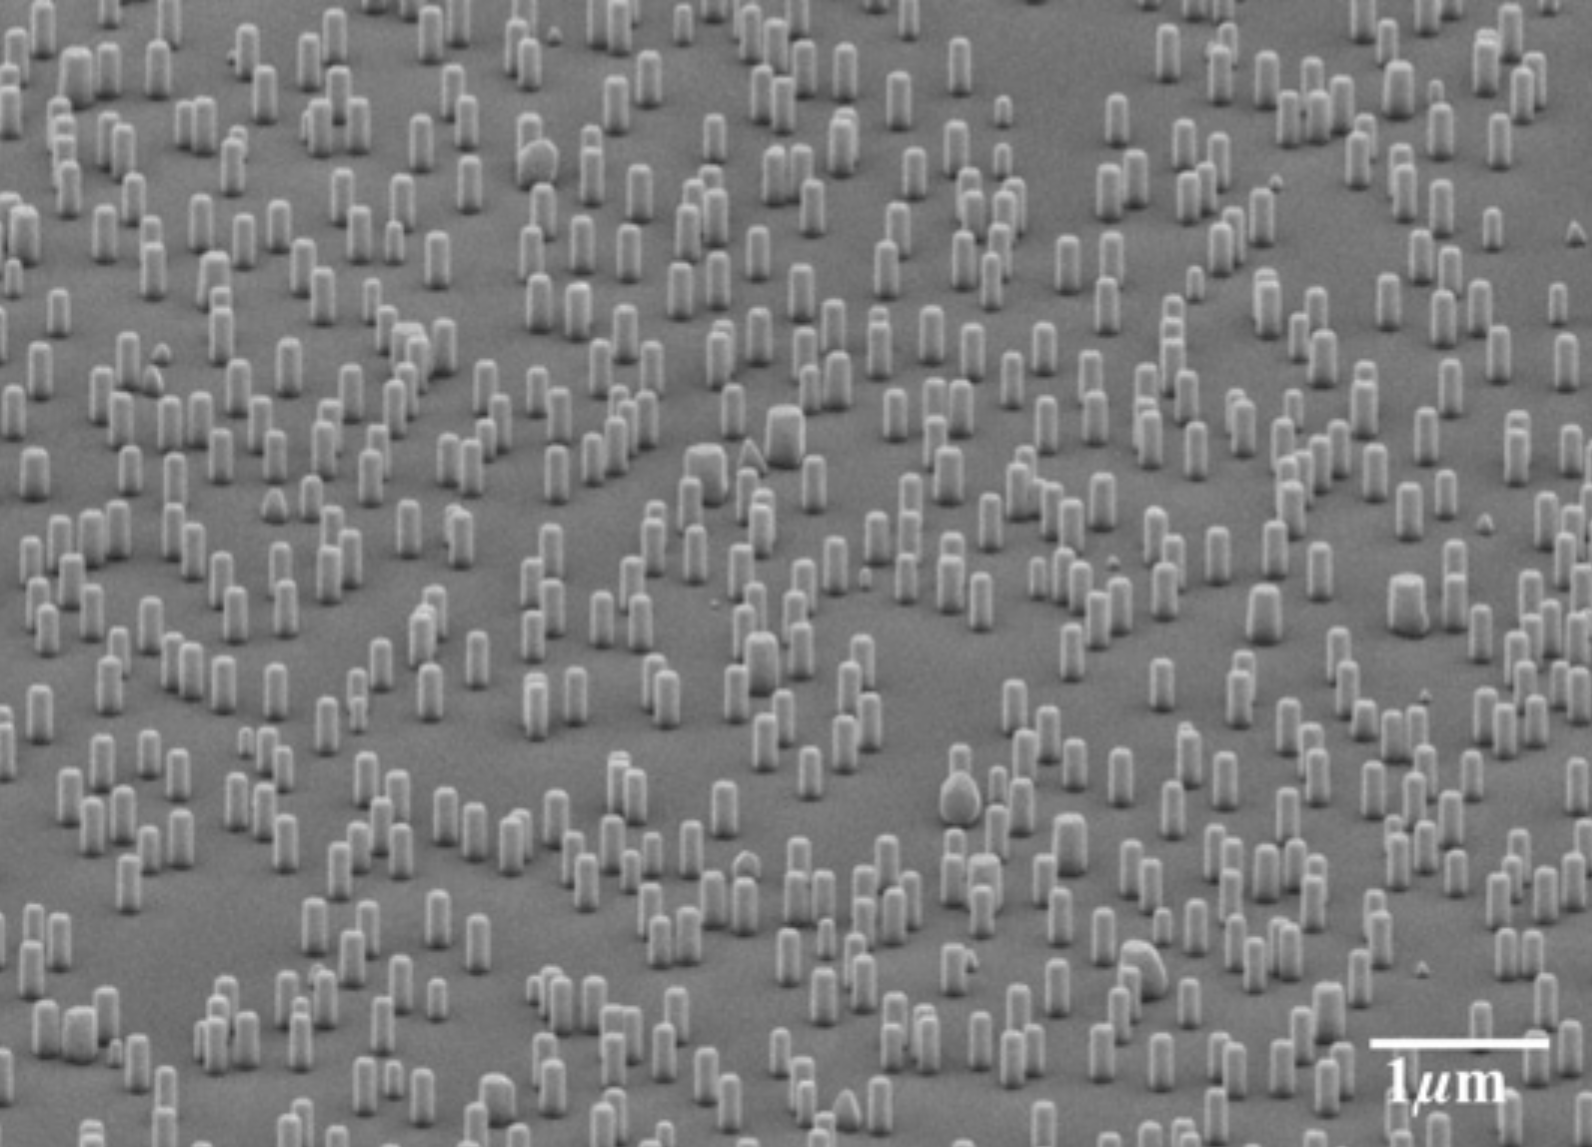
\includegraphics{nanocdte_nanowires}
        \caption{\label{fig:nanocdte_nanowires} SEM image of CdTe nanowires derived from Bi2 Te3
            catalytic seeds presented from a 70\degree~tilt side view.}
    \end{subfigure}
    \caption{\label{fig:nanocdte_sem}SEMs of seeds and resulting wires}
\end{figure}

Figure 2 shows an SEM image of the CdTe nanowires
derived from Bi\textsubscript{2}Te\textsubscript{3} seeds. In many respects, these nanowires
are indistinguishable from those grown using bismuth seeds
in conjunction with an alcohol-altered surface [19]. The two
methods both yield vertically aligned nanowires that are highly
faceted, share an epitaxial relationship with the substrate and
grow without a two-dimensional planar layer. The nanowires
are identical from a structural standpoint as well, exhibiting
the wurtzite crystal structure instead of the bulk zinc blende phase. Figure 3
shows a pole figure that includes contributions from both
the (111) zinc blende and (0002) wurtzite planes. Both phases give rise to a peak in the
centre of the pole, but a zinc blende phase must also give rise to
a ring of three peaks at the outer extent of the pole. For the pole
figure shown no such peaks are observed, but in general a small
zinc blende signature was visible. The three small peaks that
do appear in the pole figure are associated with the sapphire
substrate.
\begin{figure}
    \centering
    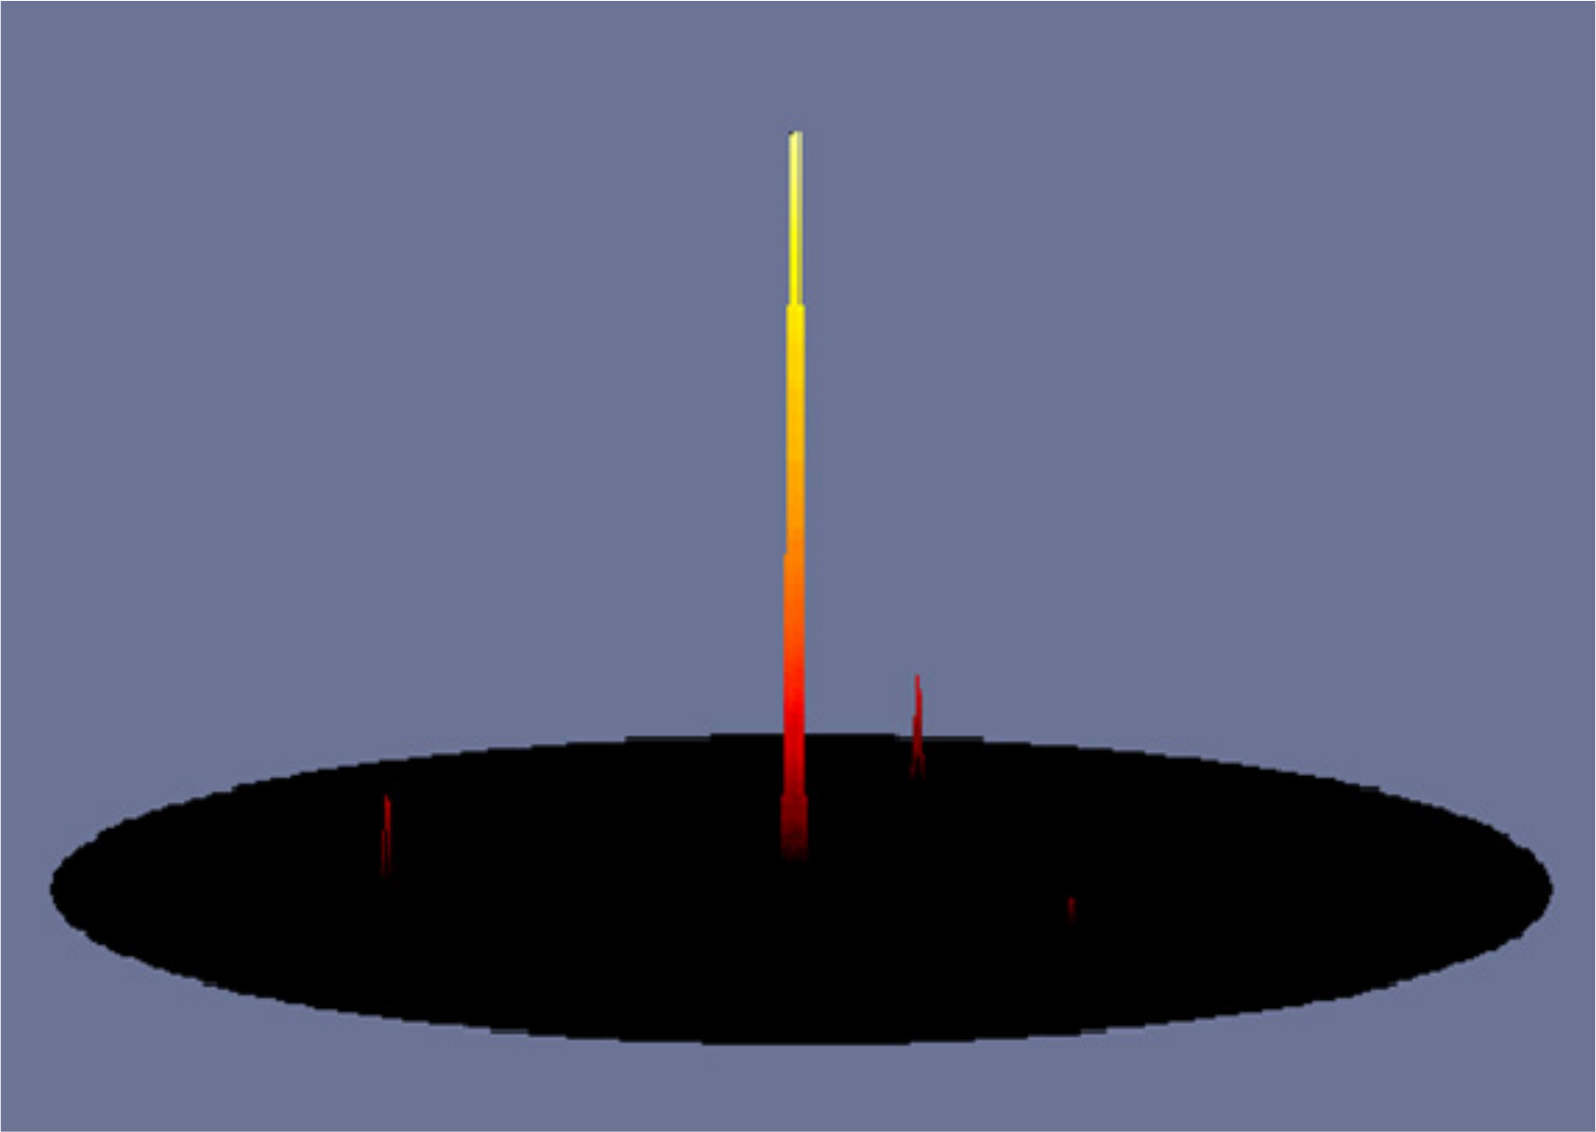
\includegraphics{nanocdte_polefigure}
    \caption{\label{fig:nanocdte_polefigure}CdTe pole figure results for 2\straighttheta~values that include contributions from both the (111) zinc blende and (0002) wurtzite phases. The pole figure shows no evidence of a zinc blende phase. The three small peaks originate from the (0001) sapphire substrate.}
\end{figure}

Even though these Bi\textsubscript{2}Te\textsubscript{3} catalysed nanowires share
many similarities with those derived from the bismuth seeds
deposited on an alcohol-altered surface, there do exist
substantial differences. One of the most striking differences
is the nanowire size distribution observed in the SEM images
of figure 4. This size distribution is quantified by the colour
map presented in figure 5(a). It shows a nanowire height
versus diameter distribution for the Bi\textsubscript{2}Te\textsubscript{3} seeded nanowires. It is quite clear from the map that larger diameter nanowires exhibit higher axial growth rates than smaller diameter ones. Figures 5(b) shows the same distribution for nanowires derived 
from bismuth seeds deposited on an alcohol-altered surface. A 
comparison of the two colour maps shows that the alcohol- 
altered surface gives rise to a significantly narrower size 
distribution. It is also apparent from the distributions that the 
Bi\textsubscript{2}Te\textsubscript{3} seeded nanowires are of larger diameter with values typically in the range of 80?200 nm. Also different is the fact that the nanowire height is not limited to 300 nm. Instead the nanowires grow longer while at the same time exhibiting
substantial growth in the lateral direction (figure 6).
Moving away from the optimum growth conditions gives
rise to other significant differences between the two nanowire
growth procedures. First, nanowires formed at the substrate's
edge have slanted tops where the direction of the slant at the
left and right edges of the substrate point in opposite directions
(figure 7). Also of note is the fact that the nanowire's cross-
section is no longer hexagonal, but instead elongates along the
direction of the slant. Second, at high growth rates Bi\textsubscript{2}Te\textsubscript{3}
seeded nanowires show significant tapering (figure 8).
\begin{figure}
    \centering
    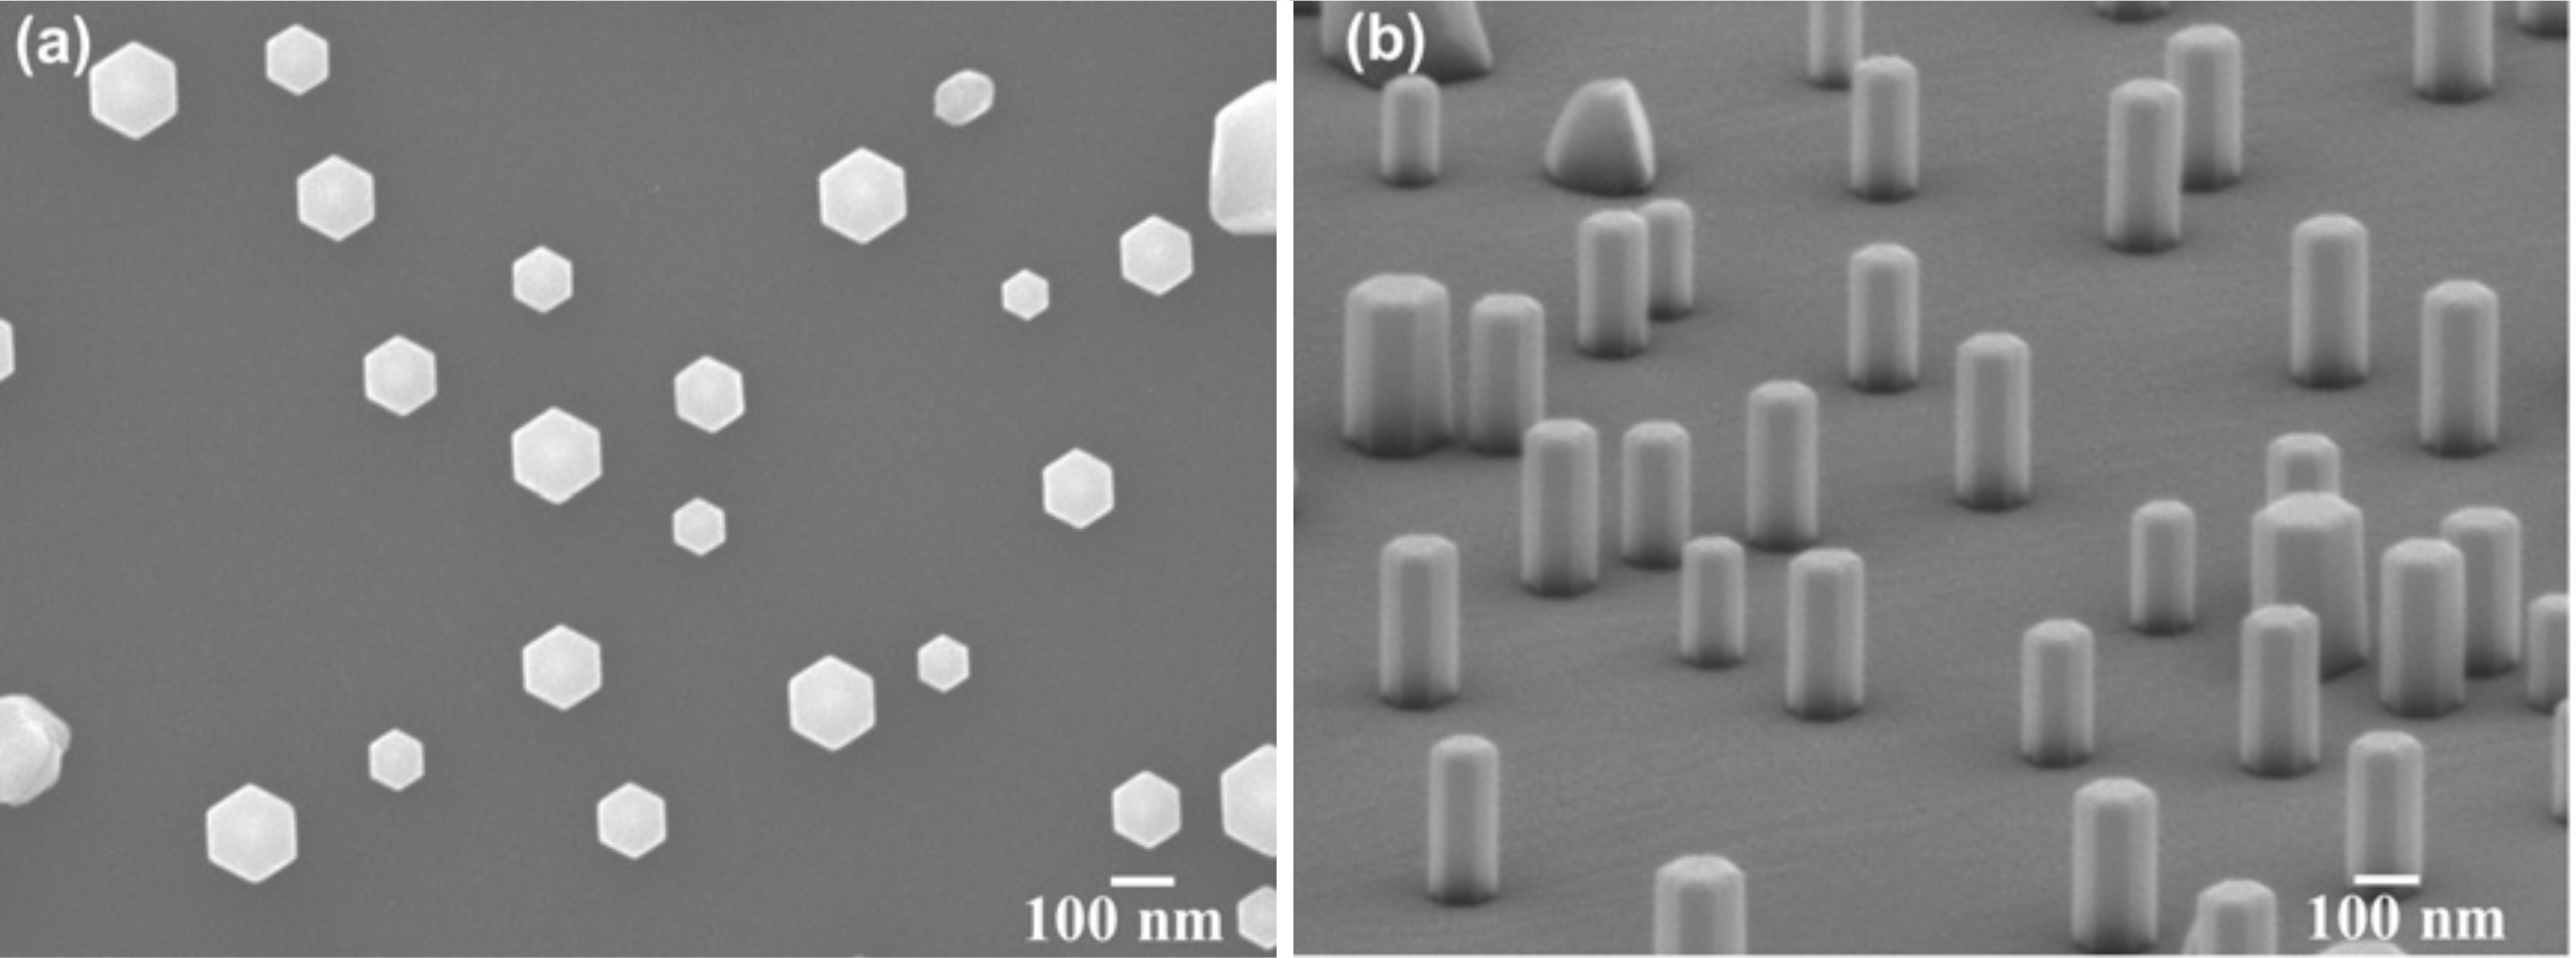
\includegraphics[width=\textwidth]{nanocdte_SEM2}
    \caption{\label{fig:nanocdte_SEM2}SEM images of CdTe nanowires from a (a) top and (b) side view (70\degree~tilt). Note that the highly faceted wires exhibit a substantial variation in both heights and diameters.}
\end{figure}
\begin{figure}
    \centering
    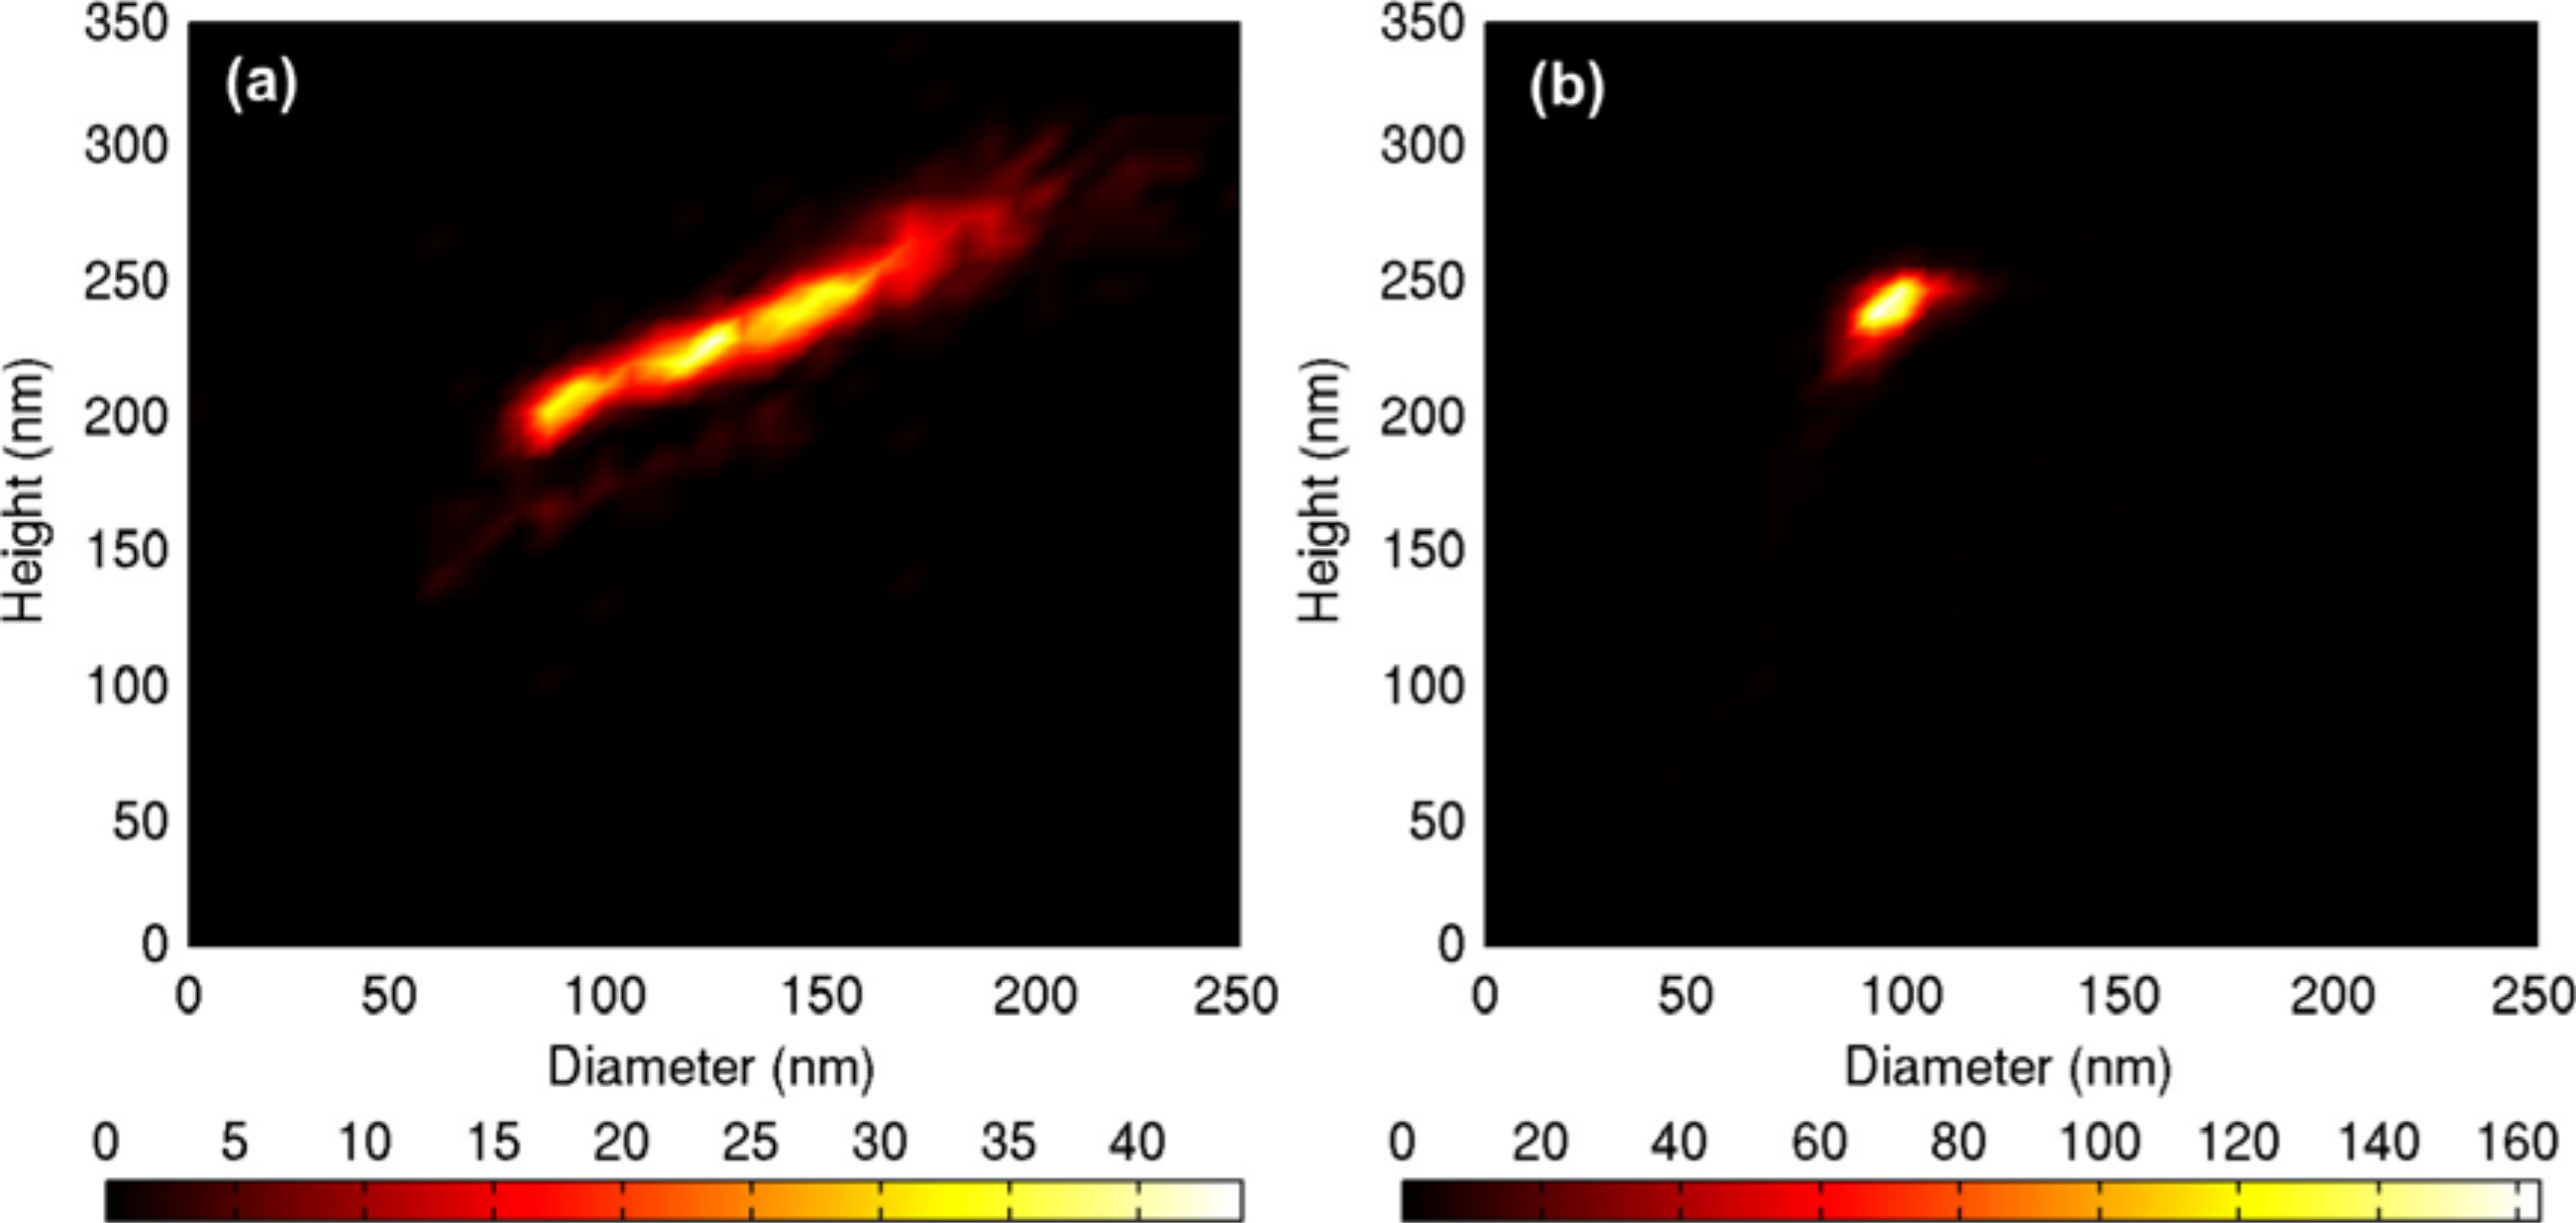
\includegraphics[width=\textwidth]{nanocdte_stats}
    \caption{\label{fig:nanocdte_stats}Colour map showing the nanowire height versus diameter size distribution for nanowires derived from (a) Bi\textsubscript{2}Te\textsubscript{3} catalytic seeds
        and (b) bismuth seeds deposited on an alcohol-altered surface. The maps were generated from the measured dimensions of (a) 1344 and
        (b) 966 nanowires. The colour bar below each figure denotes the number of times a nanowire of a given dimension is observed. Note that the
        Bi\textsubscript{2}Te\textsubscript{3} seeded nanowires exhibit a broader size distribution and sizes that are, in general, larger than the bismuth seeded wires.}
\end{figure}
\begin{figure}
    \centering
    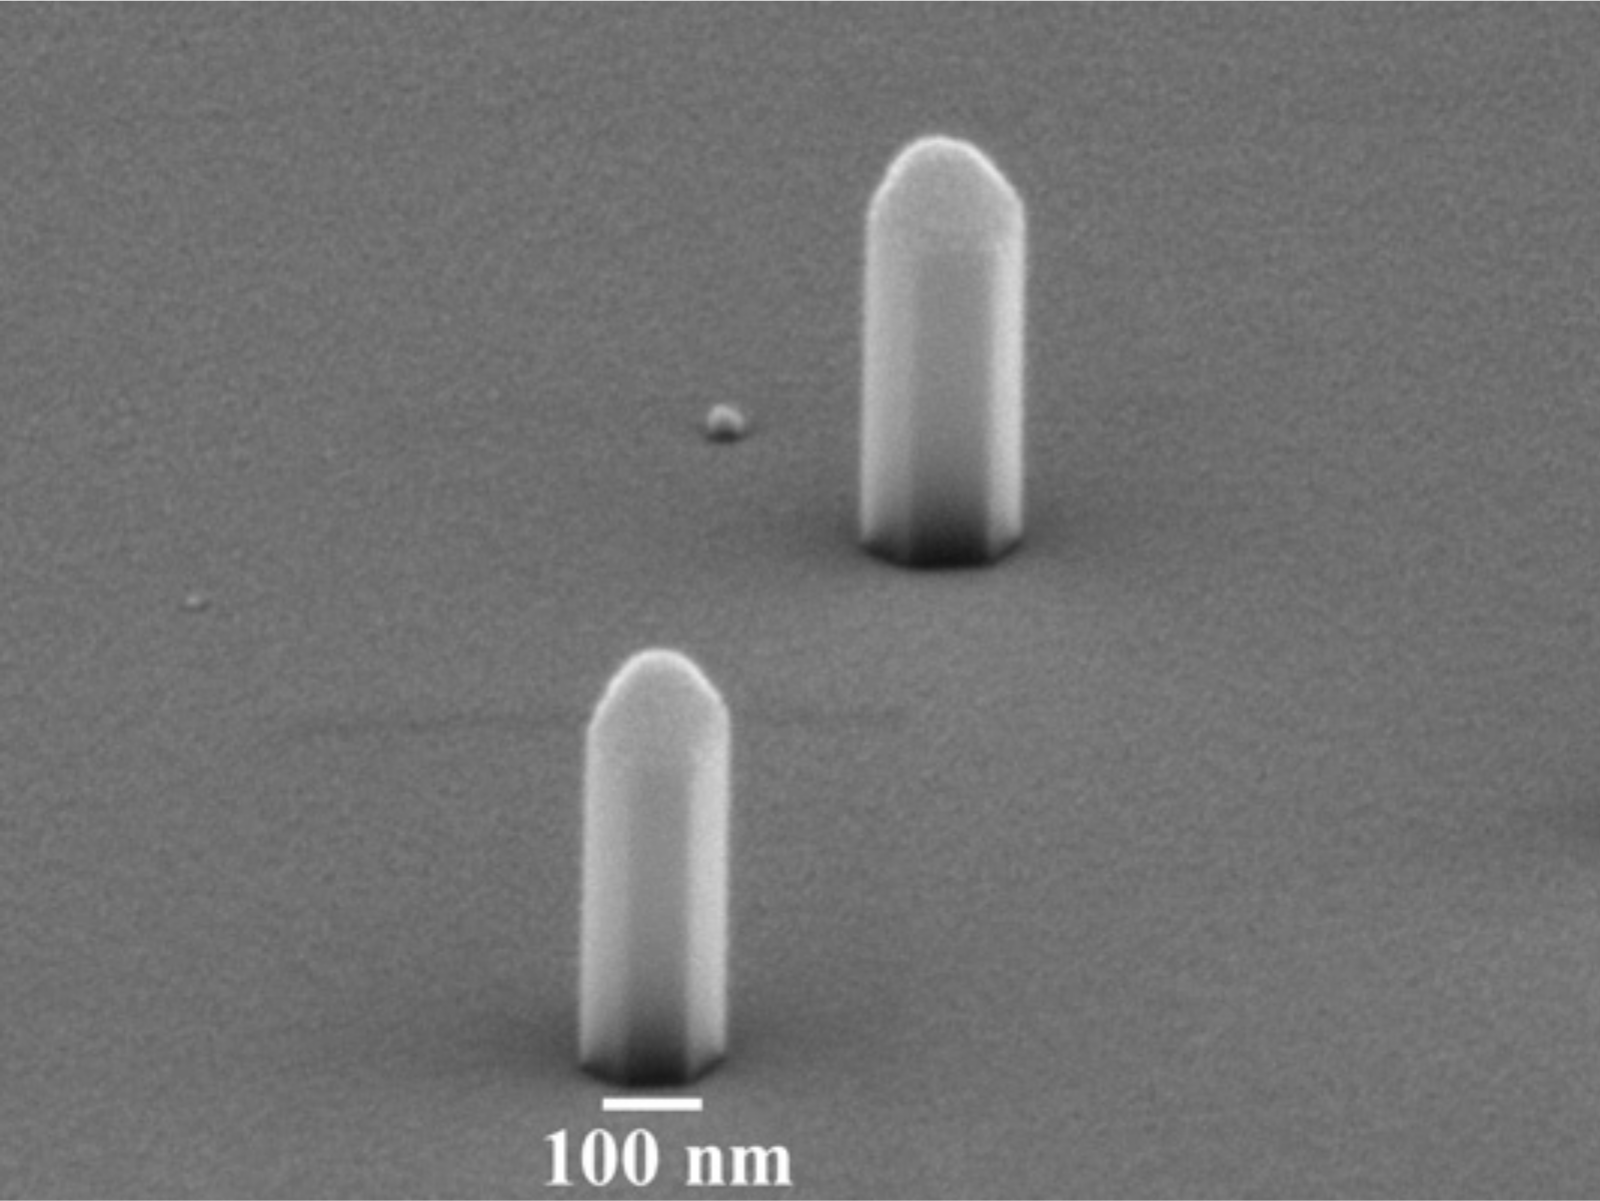
\includegraphics{nanocdte_lateral}
    \caption{\label{fig:nanocdte_lateral}SEM images of CdTe nanowires deposited using extended 
        growth times where increases to the height are met with substantial lateral growth.}
\end{figure}
\begin{figure}
    \centering
    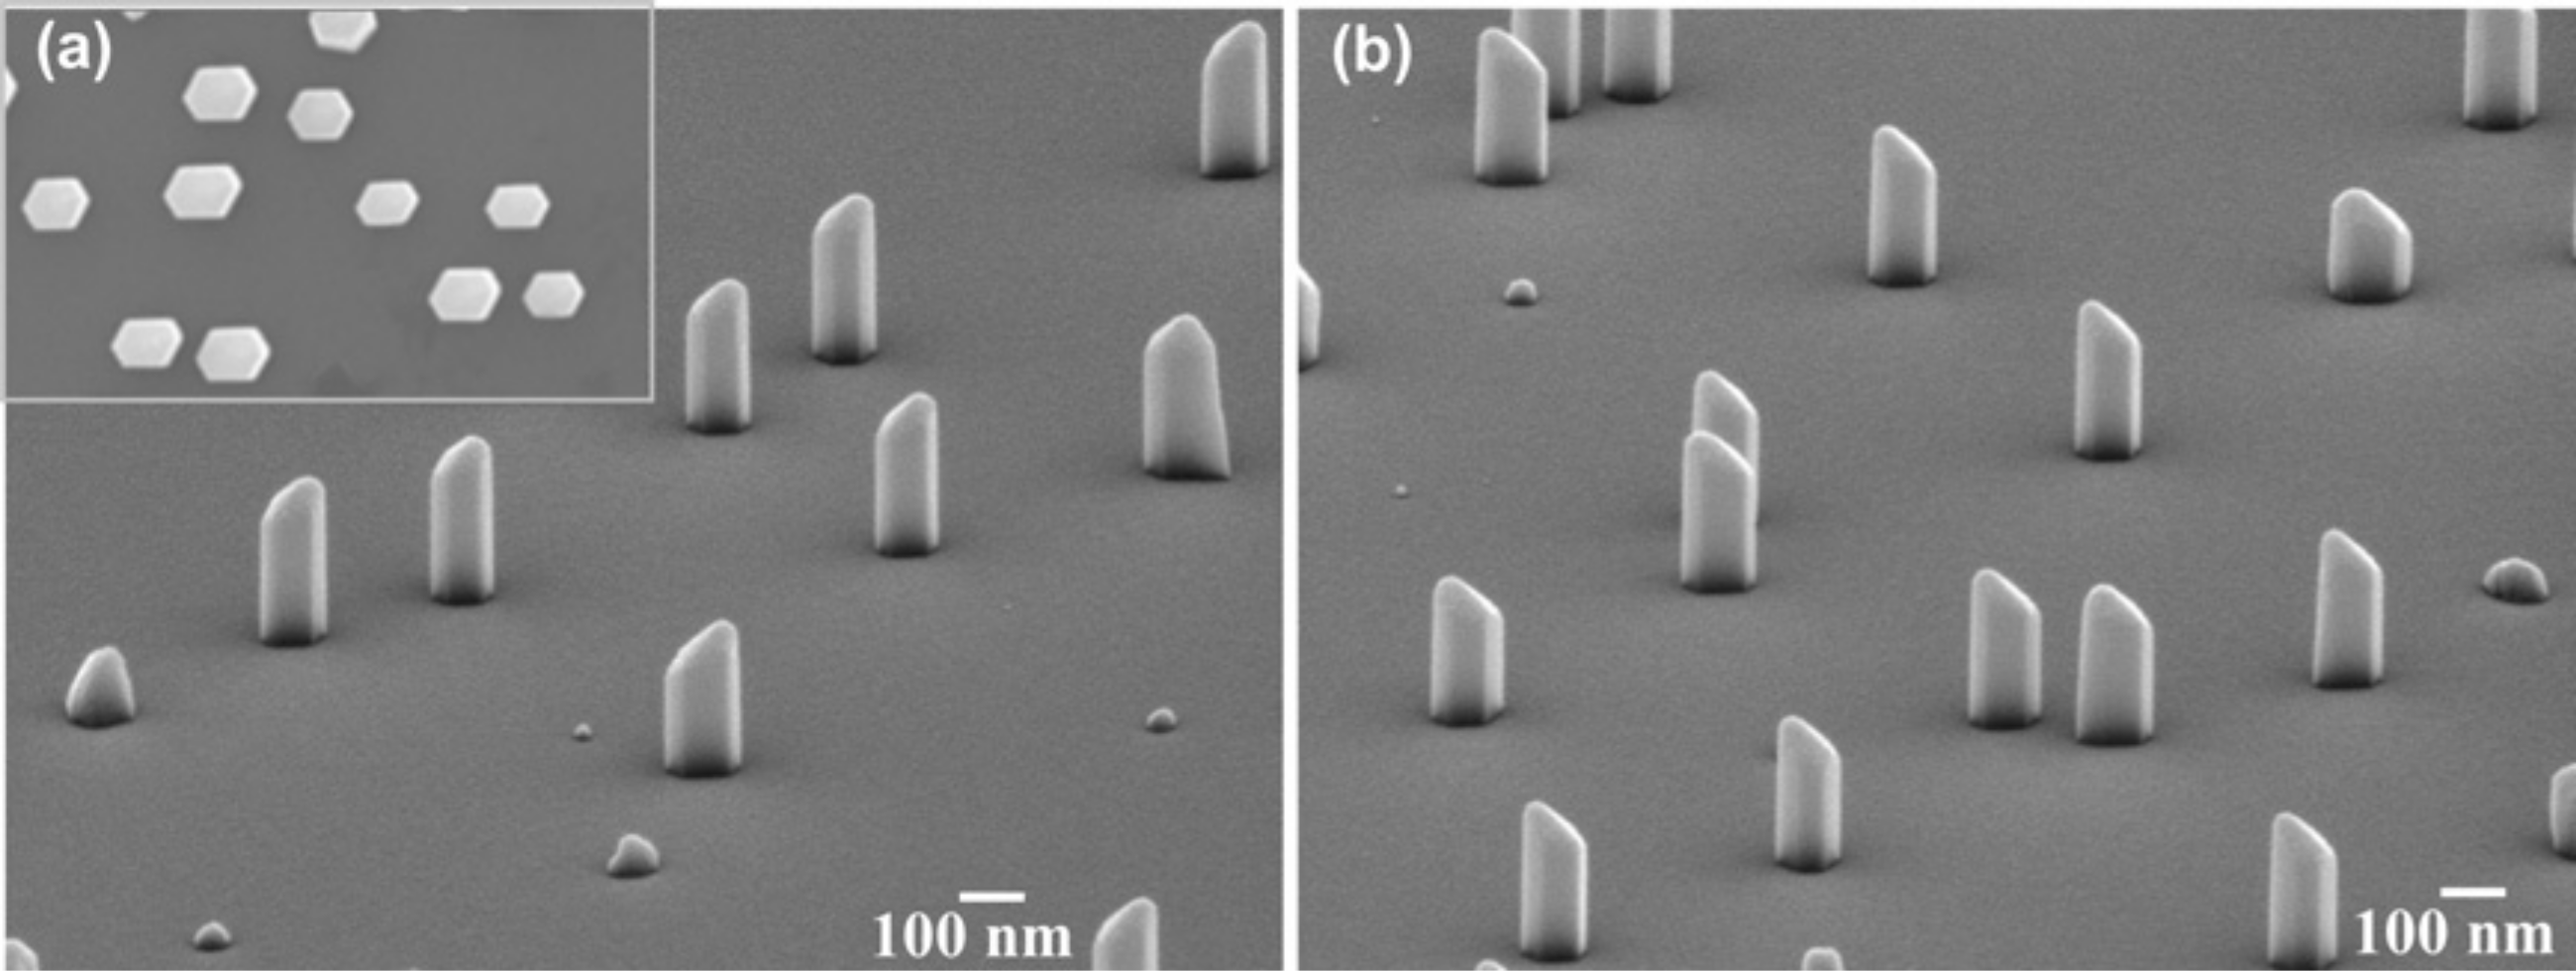
\includegraphics{nanocdte_slanted}
    \caption{\label{fig:nanocdte_slanted}SEM images of CdTe nanowires with slanted tops that have formed at the (a) left and (b) right edge of the substrate. Note that the
        tilt is in opposite directions. The top views of these nanostructures, shown in the inset to (a), indicate that the hexagonal cross-sections are
        elongated in the horizontal direction.}
\end{figure}
\begin{figure}
    \centering
    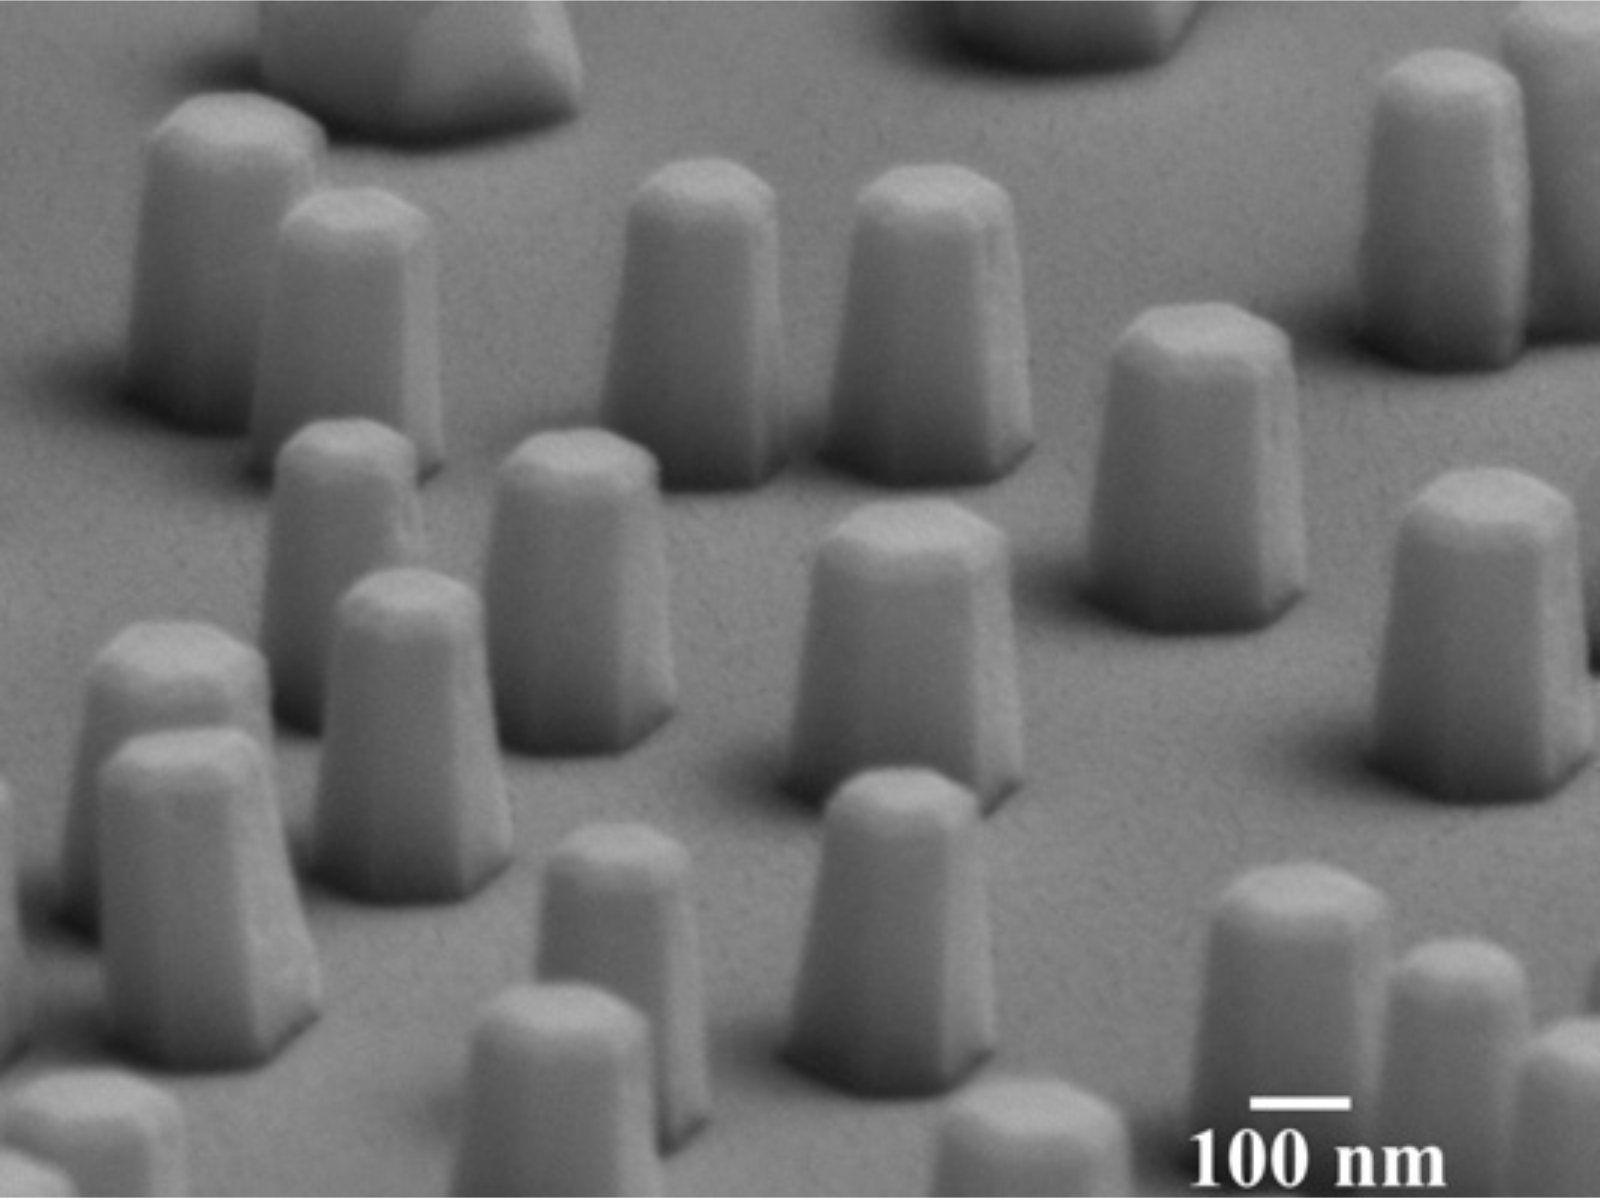
\includegraphics{nanocdte_tapered}
    \caption{\label{fig:nanocdte_tapered}SEM image showing tapered CdTe nanowires.}
\end{figure}
This work combined with our previous results has demon-
strated that CdTe nanowire structures can originate from cat-
alytic seeds derived from two separate processes, with each
of these processes having advantages and disadvantages. Bis-
muth seeds, in combination with an alcohol-altered surface,
give rise to superior nanowire uniformity, but there exist
nanowire height limitations and fabrication can only proceed
using volatile catalytic seeds maintained in a narrow window
of processing parameters. The Bi\textsubscript{2}Te\textsubscript{3} seeds are much more stable at the temperatures needed to initiate CdTe nanowire growth. This makes nanowire production possible without the
cumbersome alcohol pre-treatment of the substrate's surface.
The main disadvantage is that the nanowire size and shape distributions are severely compromised.

It is important to emphasize that well over one hundred
samples have been characterized for each of the two nanowire
deposition methods. As a result, nanowire fabrication has
been attempted over a broad range of growth conditions.
Thus, the features presented here as unique to the Bi\textsubscript{2}Te\textsubscript{3}
initiated nanowires have been shown to decisively differentiate
themselves from those observed using bismuth seeds deposited
on an alcohol-altered surface. If, as expected, both the bismuth
and Bi\textsubscript{2}Te\textsubscript{3} catalytic seeds assume the same composition once
exposed to a flux of cadmium and tellurium then the differences
observed between the two methods must be attributed to the
presence or absence of an alcohol-altered substrate surface. It
is our conjecture that this can be done within the confines of
the existing nanowire growth modes.

For both nanowire deposition methods the catalytic
seeds are derived from a thin film that dewets at elevated
temperatures. Once formed, these seeds are subject to Ostwald
ripening, where there is an exchange of atoms along the
substrate's surface with larger seeds growing at the expense
of smaller ones [21, 22]. The effectiveness of this process is
governed by the adatom's surface diffusion length given by
the square root of the product of its diffusion coefficient and
lifetime. If this length is larger than the separation between
seeds then Ostwald ripening proceeds in the usual manner
where, as time progresses, there exists an increasing variation
in seed size. On the other hand, if this length is reduced
to where atoms liberated from one seed evaporate before
encountering a second one, then a narrow size distribution will
be maintained, but accompanied by a continuous reduction in
the seed's diameter.

It is clear from our results that the pristine substrate used
for the Bi\textsubscript{2}Te\textsubscript{3} seeds leads to sufficient surface mobility for
Ostwald ripening to broaden the distribution of seed diameters.
Due to the higher volatility of tellurium we expect that this
ripening process will result in bismuth-rich seeds. Indeed, the
binary phase diagram indicates that the growth temperature is
too low for the seeds to melt unless there is first a substantial
loss of tellurium [23]. The combination of Ostwald ripening in conjunction with evaporation leads to bismuth-rich catalytic
seeds of different sizes which in turn give rise to nanowires of
varying diameters. Corrupting the surface with alcohol alters
this process by dramatically reducing the surface mobility; this
increases the lifetime of the seed on the surface and frustrates
the Ostwald ripening process, i.e., any bismuth atoms liberated
from an individual seed are backscattered to the original seed
or evaporate from the surface before reaching a second seed.
With the ripening process halted, the distribution of seed
diameters remains narrow, ultimately giving rise to a narrow
distribution of nanowires.

With the catalytic seeds in place and exposed to a
flux of cadmium and tellurium atoms it is expected that
both the bismuth and Bi\textsubscript{2}Te\textsubscript{3} seeds will evolve to the same
ternary composition. While the ternary phase diagram for
the cadmium/tellurium/bismuth system is unknown, it is well
established that individually both tellurium and cadmium are
soluble in bismuth [23]. The catalytic seed's ability to stabilize
both elements on the timescales necessary for CdTe formation
is crucial. This is made evident by the fact that the CdTe
nanowires grow in the absence of a two-dimensional planar
layer. This is attributable to the fact that both cadmium and
tellurium have negligible sticking coefficients at the substrate
temperature used. It is only through the formation of CdTe
that these species have significant lifetimes on the substrate's
surface. For the growth conditions used, however, the adatom
lifetimes are too small to enable CdTe formation directly on the sapphire negating a planar growth mode. As a result, CdTe growth can only proceed through the catalytically
driven process. Consistent with this analysis is a nanowire
height distribution with the tallest nanowires having the largest
diameters. This is in contrast to substrate-based nanowire
growth modes where the tallest nanowires are those with the
smallest diameters. For these systems, the nanowire height
distribution is driven by adatoms arriving at the substrate's
surface and making their way to the growth front via a random
walk that takes them up the nanowire's sidewalls. For the CdTe
case, the small adatom lifetime negates this process resulting
in a nanowire growth mode that is dependent upon the direct
impingement of atoms onto the catalytic seeds. Such a growth
mode is not commonly observed in semiconductor nanowire
systems.
\begin{figure}
    \centering
    \begin{subfigure}[t]{0.5\textwidth}
        \centering
        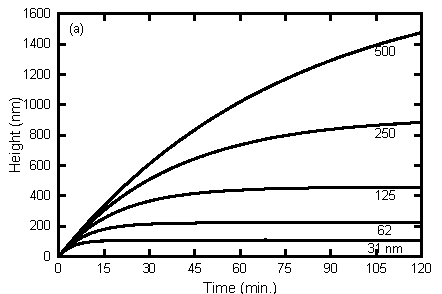
\includegraphics{nanocdte_model_thickness}
        \caption{\label{fig:nanocdte_model_thickness}}
    \end{subfigure}%
    \begin{subfigure}[t]{0.5\textwidth}
        \centering
        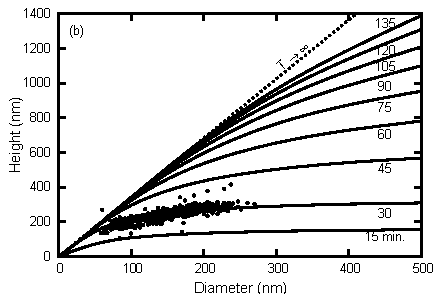
\includegraphics{nanocdte_model_time}
        \caption{\label{fig:nanocdte_model_time}}
    \end{subfigure}
    \caption{\label{fig:nanocdte_model}Simulation results showing (a) the time evolution of the nanowire height for the five labelled diameters and (b) time snapshots of the
        height versus diameter dependence for the times labelled. The dashed line shows the linear dependence expected when all nanowires reach an
        equilibrium condition. Superimposed over the simulation is the experimental data (black dots) of figure 5(a). The values used in this
        simulation have been scaled so as to fit this experimental distribution.}
\end{figure}

A growth mode driven by direct impingement, where all
the adatoms arrive normal to and are incorporated into the
nanostructure, will result in a nanowire height distribution
that is independent of diameter. There are, however, other
factors that can come into play. It has been demonstrated
both experimentally [24, 25] and theoretically [10, 13] that the
Gibbs?Thomson effect can give rise to a height distribution
directly proportional to the nanowire diameter. The effect
stipulates that the higher curvature associated with smaller
diameter seeds yields a higher effective vapour pressure,
reducing the uptake of atoms from the impinging vapour.
While this effect qualitatively gives rise to the observed CdTe
nanowire height distribution, it is unable to account for the
observed height limitation for the bismuth seeded nanowires
as it provides no means of halting the growth.

The self-limiting growth mode displayed by the bismuth
seeded nanowires deposited on an alcohol-altered surface
likely originates from an equilibrium that develops between the
addition of adatoms through direct impingement on the catalyst
and the loss of atoms from the sidewalls through sublimation.
The sublimation process is significant for the CdTe nanowires
as they will disappear completely in approximately 30 min if
left at the growth temperature in the absence of an incoming
flux of cadmium and tellurium atoms. A similar situation must
exist for the Bi\textsubscript{2}Te\textsubscript{3} seeded nanowires, but in this case the results are complicated by the distribution of the nanowires'
diameters and the lateral growth that becomes apparent for
long growth times. A stochastic simulation was conducted
to show the time evolution of the nanowires subject to a
sublimation process. With the uptake of material being
proportional to the area of the catalytic seed and the loss of
material being proportional to the area of the sidewalls, the
simulation yields nanowire heights showing the time evolution
presented in figure 9(a). Snapshots in time of the nanowire
height versus diameter distribution are shown in figure 9(b)
with the experimentally observed distribution of figure 5(a)
superimposed. The intent of this simulation was not to
rigorously model the nanowire growth as it ignores such factors
as the Gibbs?Thomson effect. It does, however, demonstrate
that sidewall sublimation limits nanowire height and results
in a size distribution qualitatively similar to that observed
experimentally.

Essential to this work is the observation that Bi\textsubscript{2}Te\textsubscript{3} seeded
nanowires show a marked tendency towards lateral growth,
while the bismuth seeded nanowires deposited on an alcohol-
altered substrate do not. This tendency is displayed not only
at long growth times, but also in the tapering shown at high
growth rates and in the elongation of the slanted-top nanowires
formed at the edge of the substrates. These three observations
are consistent with the preferential nucleation of adatoms at the
base of the nanowire where a weak nucleation site forms due to
atomic bonding from both the sidewall facet and the substrate.
Such a nucleation site would be analogous to the ones formed
on a vicinal substrate [26]. The atoms forming at the base
would then have to promote the propagation of a layer up the
nanowire's sidewall. The existence of a lateral growth mode
accounts for the formation of tall, large diameter nanowires
for extended growth times (figure 6). In the initial stages of
growth the axial growth rate exceeds the lateral growth rate by
a wide margin, but as the nanowire approaches its height limit
the axial growth slows dramatically as shown in figure 9(a).
The model presented, however, does not account for the
situation where a slow lateral growth mode accompanies the
axial growth. In this scenario, lateral growth results in larger
diameter nanowires which, in turn, allow for increased axial growth. As a result, both dimensions will grow slowly in
tandem provided that the catalytic material remains active as
it spreads out over the expanding top surface of the nanowire.

Lateral growth is most evident for the slanted-top
nanowires (figure 7) as it proceeds in an anisotropic manner.
In the PLD process cadmium and tellurium atoms exit the
target from an area a few square millimetres in diameter.
Thus, while the ablated material arrives normal to the centre
of the substrate, it arrives at an angle to the edges. As a
result, nanowires growing at the edges will have cadmium and
tellurium atoms preferentially landing on the sidewall facet
nearest to the centre of the substrate. Thus, the adatoms have
an increased likelihood of becoming a part of both the growth
front nearest to that sidewall facet as well as to any layer
propagating up that sidewall. It is this asymmetry that leads
to the anisotropic growth mode that is mirrored on opposite
sides of the substrate.

The extent of the lateral growth at the base of the nanowire
must be contingent upon the availability of adatoms on the
surface of the substrate. At slow growth rates the nucleation
of adatoms will be far more difficult as singly bonded atoms
and small clusters of atoms will easily dissociate, making
them prone to evaporation from the surface. At higher growth
rates the availability of adatoms increases allowing for larger
clusters to stabilize. Under these conditions the nanowires will
have a small, but significant, collection area. The effect of
this collection area, however, will diminish as one moves away
from the surface of the substrate, a situation that should give
rise to a tapered structure as shown in figure 8.

As previously mentioned, these lateral growth modes are
absent for the bismuth seeded nanowires deposited on an
alcohol-altered substrate. It is our conjecture that during the
dewetting process, the bismuth seeds are able to penetrate
through this surface-altered layer in a manner that effectively
cleans the surface and exposes the (0001) face of sapphire;
a face essential to the epitaxial alignment of the nanowires.
This statement is supported by the fact that a bismuth
absorption/desorption treatment has been used to remove
carbon-containing impurities from the surface of SrTiO3 and
LaAlO3 [27]. However, around the periphery of each seed it is
expected that the substrate's alcohol surface alteration persists.
As a result, the nucleation site at the base of the nanowire is of
poor quality as the substrate's epitaxial relationship no longer
exists due to the corrupted surface. It is this deterioration
in the nucleation site that inhibits the nanowire's ability to
grow laterally. In general, poor adhesion of adatoms to the
substrate should be quite detrimental to a lateral growth mode
as adatoms must already have a low probability of attaching to
the sidewall facet; if this were not the case a one-dimensional
nanowire growth mode would be unattainable. It should be
noted that the described process results in lateral overgrowth
suppression in a manner analogous to that used for nanowire
production through the use of selective area epitaxy. It is well
established that CdTe is prone to such a process as there exists
a substantive body of work detailing procedures for obtaining
selective epitaxy in the CdTe system [28-30]. Also supportive
of this explanation are reports detailing the fabrication of
vertically aligned nanowires, where non-vertically aligned
growth is eliminated through the use of organic layers [31-33].


\section{Implications for Symmetry and Energy at Epitaxial Surfaces} 
\chapter{III-V Growth on Oxides and Liftoff Phenonmoon}
%\section{Introduction}

\section{Background}

\section{Experimental}

\section{Results and Discussion}

\section{Implications for Symmetry and Energy at Epitaxial Surfaces}
\part{Noble Metals on Oxides}
\chapter{Nanostructured Gold on Spinel}
%\section{Introduction}
As part of the investigations into VLS growth of CdTe nanowires, the control of the size and spatial distribution of metal seeds on oxides was investigated. CdTe nanowire growth had been previously successful using Bi and BiTe seeds, however there are unstable, gold or another noble metal would expand the processing window both in terms of time and temperature. As such, experiments into the control of gold on several oxide substrates was undertaken.

While ultimately nanowire growth was suspendend in favour of other investigations, the research into the interactions of gold overlayers on MgAl\(_2\)O\(_4\) (spinel) substrates yielded some surprising results. The standard method of producing metal seed particles is thermal dewetting, relying upon the relative surface energies of metal versus substrate to cause the film to ball up. The dewetting of gold on spinel substrates was found to result in epitaxial alignment and nanocrystal formation. A full characterization into the formation process of the gold nanocrystals was undertaken and a phenomenological model of their formation was presented.

\section{Experimental}
The gold nanostructures were formed through the deposition of gold films on MgAl\textsubscript{2}O\textsubscript{4} substrates (MTI Corp.)
followed by an annealing procedure which facilitated film
dewetting and nanostructure formation. The films were
sputter-coated at room temperature to a thickness of 5 \AA-15
\AA with a GATAN PECS Model 682 ion beam coating/etching system. The samples were then placed in a tube
furnace with a 100 SCCM flow of argon, heated to 1100 \celsius{}
in 45 min, and then held at that temperature for 1 h.
Following this treatment, the sample was cooled to 1000 \celsius{}
in 30 min, held at that temperature for an additional hour,
and then allowed to cool to room temperature over an interval
of approximately 8 h. Holding the temperature at both 1100
and 1000 \celsius{} was crucial to the formation of the nanostructures described here. Removal of either step results in the formation of faceted gold spheres sitting directly on the substrate.

Scanning electron microscopy (SEM) images of the gold
nanostructures formed on the (100), (111), and (110)
MgAl\textsubscript{2}O\textsubscript{4} substrates, obtained using a JEOL-7000F SEM in
secondary electron mode, are shown in \cref{fig:nanogold_sem}. For each
substrate orientation, one observes two types of features, (i)
spheres supported by a necking region attached to a geometrically shaped base (\cref{fig:nanogold_sem}a-c) and (ii) standalone base
structures (\cref{fig:nanogold_sem}d-f). Convergent beam electron diffraction (CBED) performed using a Phillips CM12 confirmed
that the supported spheres are crystalline. For each case, the shape of the base structure reflects the underlying symmetry
of the substrate which is four-fold, three-fold, and two-fold
symmetric for the (100), (111), and (110) surfaces, respectively. X-ray diffraction measurements, using a Bruker 6000
CCD detector on a Bruker three circle D8 goniometer with
a Rigaku RU-200 rotating anode Cu KR X-ray generator and
parallel-focusing mirror optics, were used to determine the
substrate orientation relative to the edges of the base
structures and are denoted on the three top-down SEM
images (\cref{fig:nanogold_sem}d-f).
\section{Results and Discussion}
The crystallographic alignment of
the nanostructures is a clear indication of epitaxy and
is strongly suggestive of {111} gold faceting of the base
structures associated with the [100]- and [111]-oriented
substrates. For the (110) surface, the standalone base
structures are ill-defined and show no obvious faceting, while
those formed in combination with a sphere show shapes
consistent with mixed faceting, possibly having {111} and
{100} facets for the short and long dimension, respectively.
The standalone base dimensions are remarkably uniform with
side lengths of 40, 65, and 65 nm \(\times\) 110 nm for the (100),
(111), and (110) substrates, respectively.
\begin{figure}
    \centering
    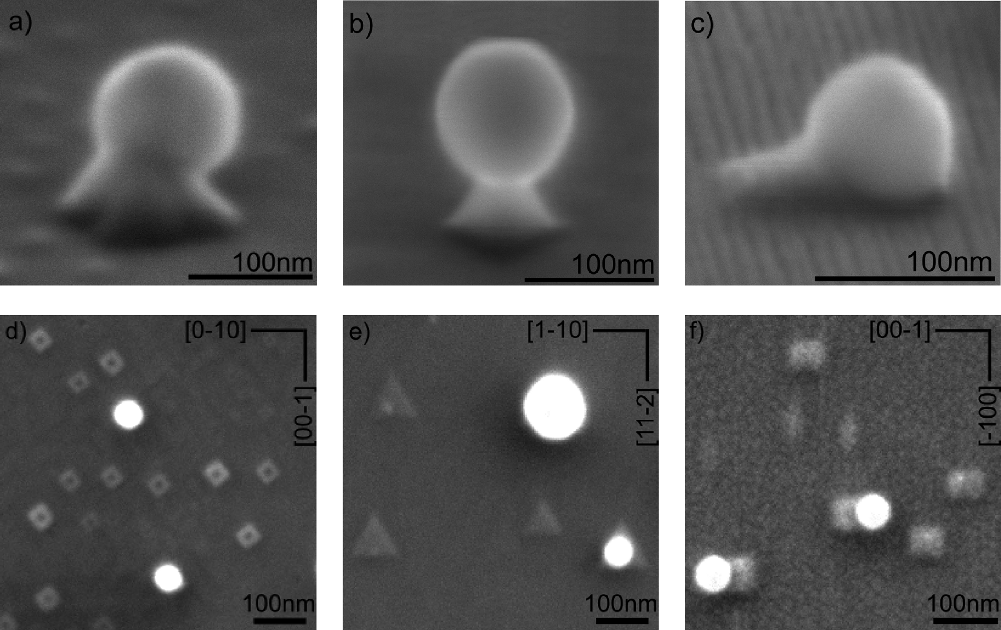
\includegraphics[width=0.8\textwidth]{nanogold_sem}
    \caption[SEM images of gold nanostructures]{\label{fig:nanogold_sem}SEM images showing the gold nanostructures formed
        on MgAl\textsubscript{2}O\textsubscript{4} substrates. The three upper images show spheres
        supported by a necking region attached to a geometrically shaped
        base for the (a) [100]-, (b) [111]-, and (c) [110]-oriented substrates.
        Each of these images was taken at a 70\degree tilt. The aura seen around
        nanostructures is an artifact of imaging. The three lower images
        show the top-down view of both standalone base structures and
        supported spheres for the (d) [100]-, (e) [111]-, and (f) [110]-
        oriented substrates. The in-plane Miller indices of the substrate are
        denoted on each of these images. For all cases, the samples were
        coated with a thin layer of platinum to improve imaging. Imaging
        without platinum shows the same structures but is of poor quality
        due to substrate charging effects.}
\end{figure}

While there are two basic types of nanostructures formed
on each substrate orientation, these structures are found in
various stages of development. For the most part, the bases
are well-developed and show little size variation. The
spherical structures, however, vary dramatically both in their
size and position relative to the base structures. \cref{fig:nanogold_progression} shows a series of top-down SEM images for the case of the
(111) MgAl\textsubscript{2}O\textsubscript{4} substrate showing an evolution of the
nanostructures from a standalone triangular base to bases
supporting spheres of increasing size. Notable is the fact that
the nanostructure, shown in \cref{fig:nanogold_progression}b, manifests itself as a
small sphere which is offset from the centre of the base while for the larger spheres, this asymmetry disappears. Such
asymmetries are observed for all three substrate orientations,
but only those nanostructures formed on the (111) substrate
consistently show a centrally placed sphere for the large
sphere sizes. Also noteworthy is a systematic effect whereby
the size of the triangular base structure increases for sphere
diameters greater than 80 nm (see \cref{fig:nanogold_progression}e and f).
\begin{figure}
    \centering
    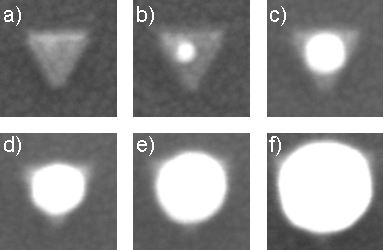
\includegraphics[width=0.9\textwidth]{nanogold_progression}
    \caption[SEM of gold nanostructure growth progression]{\label{fig:nanogold_progression}SEM images showing the top-down view of gold
        nanostructures formed on the (111) surface of MgAl\textsubscript{2}O\textsubscript{4} substrates.
        The sequence of images is chosen to show progressively larger
        spheres atop the base structures. Note that only the smallest sphere,
        shown in (b), is offset from the centre of the triangular base and
        that the base size is slightly larger when supporting larger spheres,
        as is the case for (e) and (f). The size of each image is 130\(\times\)30
        nm\textsuperscript{2}.}
\end{figure}

The base structures formed on each substrate orientation
are a clear consequence of the epitaxial relationship formed
between gold and the latticed-matched MgAl\textsubscript{2}O\textsubscript{4} substrate.
This is apparent from the fact that the geometries of the base
structures mimic the underlying symmetry of the substrates.
It is also likely that the base sizes are a consequence of the
substrate-imposed strains. Arguments based on epitaxy,
however, cannot explain the self-assembly of the gold spheres
atop the base structures and the associated necking behaviour
which facilitates their connection to the base. It is our
hypothesis that the necking behaviour results from an attempt
to minimize the surface energy of the structure. Thus, the
overall shape of these nanostructures is governed by an
interplay between the constraints imposed by epitaxy and a
requirement that the surface free energy be minimized. This
situation has much in common with formation of soap
bubbles affixed to a wire frame\cite{RefWorks:95}. This statement is based
on the facts that the frame imposes a constraint analogous
to that imposed by lattice mismatch and that the shape of
the soap bubble is, to a large degree, determined by the
surface free energy. This analogy provided the impetus for
applying the well-developed models associated with soap
bubble formation to the nanostructures described here. Such
modelling has also been successfully used to predict the
equilibrium shape of biological lipid bilayers (blood cells)
when exposed to abnormal pressure, temperature, magnetic,
and chemical environments\cite{RefWorks:99,RefWorks:102,RefWorks:47,RefWorks:100,RefWorks:101,RefWorks:103}.

The gold nanostructures were modelled as a continuum
elastic surface constrained by a footprint. Three different
footprint geometries (square, equilateral triangle, and rectangle) were used in order to mimic the four-fold, three-fold,
and two-fold symmetries associated with the (100), (111), and (110) surfaces of MgAl\textsubscript{2}O\textsubscript{4}. The size and shape of the
footprint were kept constant during the simulated growths
in order to match the experimental observation indicating a
high degree of base uniformity. For each orientation, the
contact angle (i.e., the angle between the footprint plane and
the tangent plane of any surface connected to the footprint's
edge) was set to a constant where the value was chosen to
be consistent with the observed faceting, as is schematically
shown in \cref{fig:nanogold_facets}.

With these constraints, the shape of an open elastic surface
can be fully described by the mean curvature, H, and the
Gaussian curvature, \(K\), while its corresponding elastic
properties can be characterized by a bending modulus \textkappa and
a Gaussian modulus \textkappa\textsubscript{G}. The surface energy (\(F\)) can then be
formulated as
\begin{equation}
F = \int \frac{\kappa}{2}H^2 dA + \int \kappa_G K dA + \lambda S + PV
\end{equation}
where \textlambda, V, S, and dA are the particle's surface tension,
volume, total surface area, and surface area element, respectively\cite{RefWorks:49,RefWorks:97}. The pressure, P, serves as a Lagrange multiplier
which ensures that a constant volume is enclosed between
the structure and the footprint plane. The second term gives
the integrated Gaussian curvature, which is constant according to the Gauss-Bonnet theorem\cite{RefWorks:98}. For a given surface
tension and volume, the equilibrium shape will correspond
to an energy minimum determined by the shape equation
\textdelta{} F \(=\) 0. The structures are more readily solved by first
rescaling the free energy of the model to become dimensionless, such that
\begin{equation}
\tilde{F} = \int \left (\frac{\tilde{\kappa} \tilde{H}^2}{2} + 1 \right)d \tilde{A} + \tilde{P} \tilde{V}
\end{equation}
where
\begin{align*}
\tilde{A} &= A/S_0 & \tilde{V} &= V/S^{3/2}_0 & \tilde{H} &= H S^{1/2}_0 \\
\tilde{\kappa} &= \kappa / \lambda S_0 & \tilde{P} &= P S^{1/2}_0 / \lambda & \tilde{F} &= F / (\lambda S_0)
\end{align*}
and S0 is the area of the base. Thus, according to this
dimensionless free-energy expression, there are two independent controlling parameters,
\(\tilde{\kappa}\) and \~{P}.

Helfrich and Ou-Yang\cite{RefWorks:49} have analytically solved the shape
equation for some symmetrical geometries. For the work
presented here, the surface is sectioned into discrete elements
using a triangulation mesh, and a simple dissipative model
is used to minimize the energy, as in eq 2\cite{RefWorks:76}
\begin{equation}
    \frac{\delta \mathbf{r}}{\delta t} = - M \frac{\delta \tilde{F}}{\delta \mathbf{r}}
\end{equation}
where \textbf{r}(t) is the position vector of a point on the particle
surface at the time t and M is a kinetic coefficient. These
methods, developed by Taniguchi et al.\cite{RefWorks:76}, are, however,
unable to simulate large deformations. To circumvent this
limitation, we employed two techniques, equiangulation and
vertex averaging, available through the Surface Evolver software developed by K. Brakke.49 Following the procedure of Lim et al.,39,42,43 the curvature was discretized based on
the methods of Julicher,50 which exactly describe the
curvature in the continuum limit. The variational derivative
used in the triangulation scheme was evaluated analytically.
For the Surface Evolver technique, variables were solved
numerically when analytical variations for discrete curvatures
proved difficult.
\begin{figure}
    \centering
    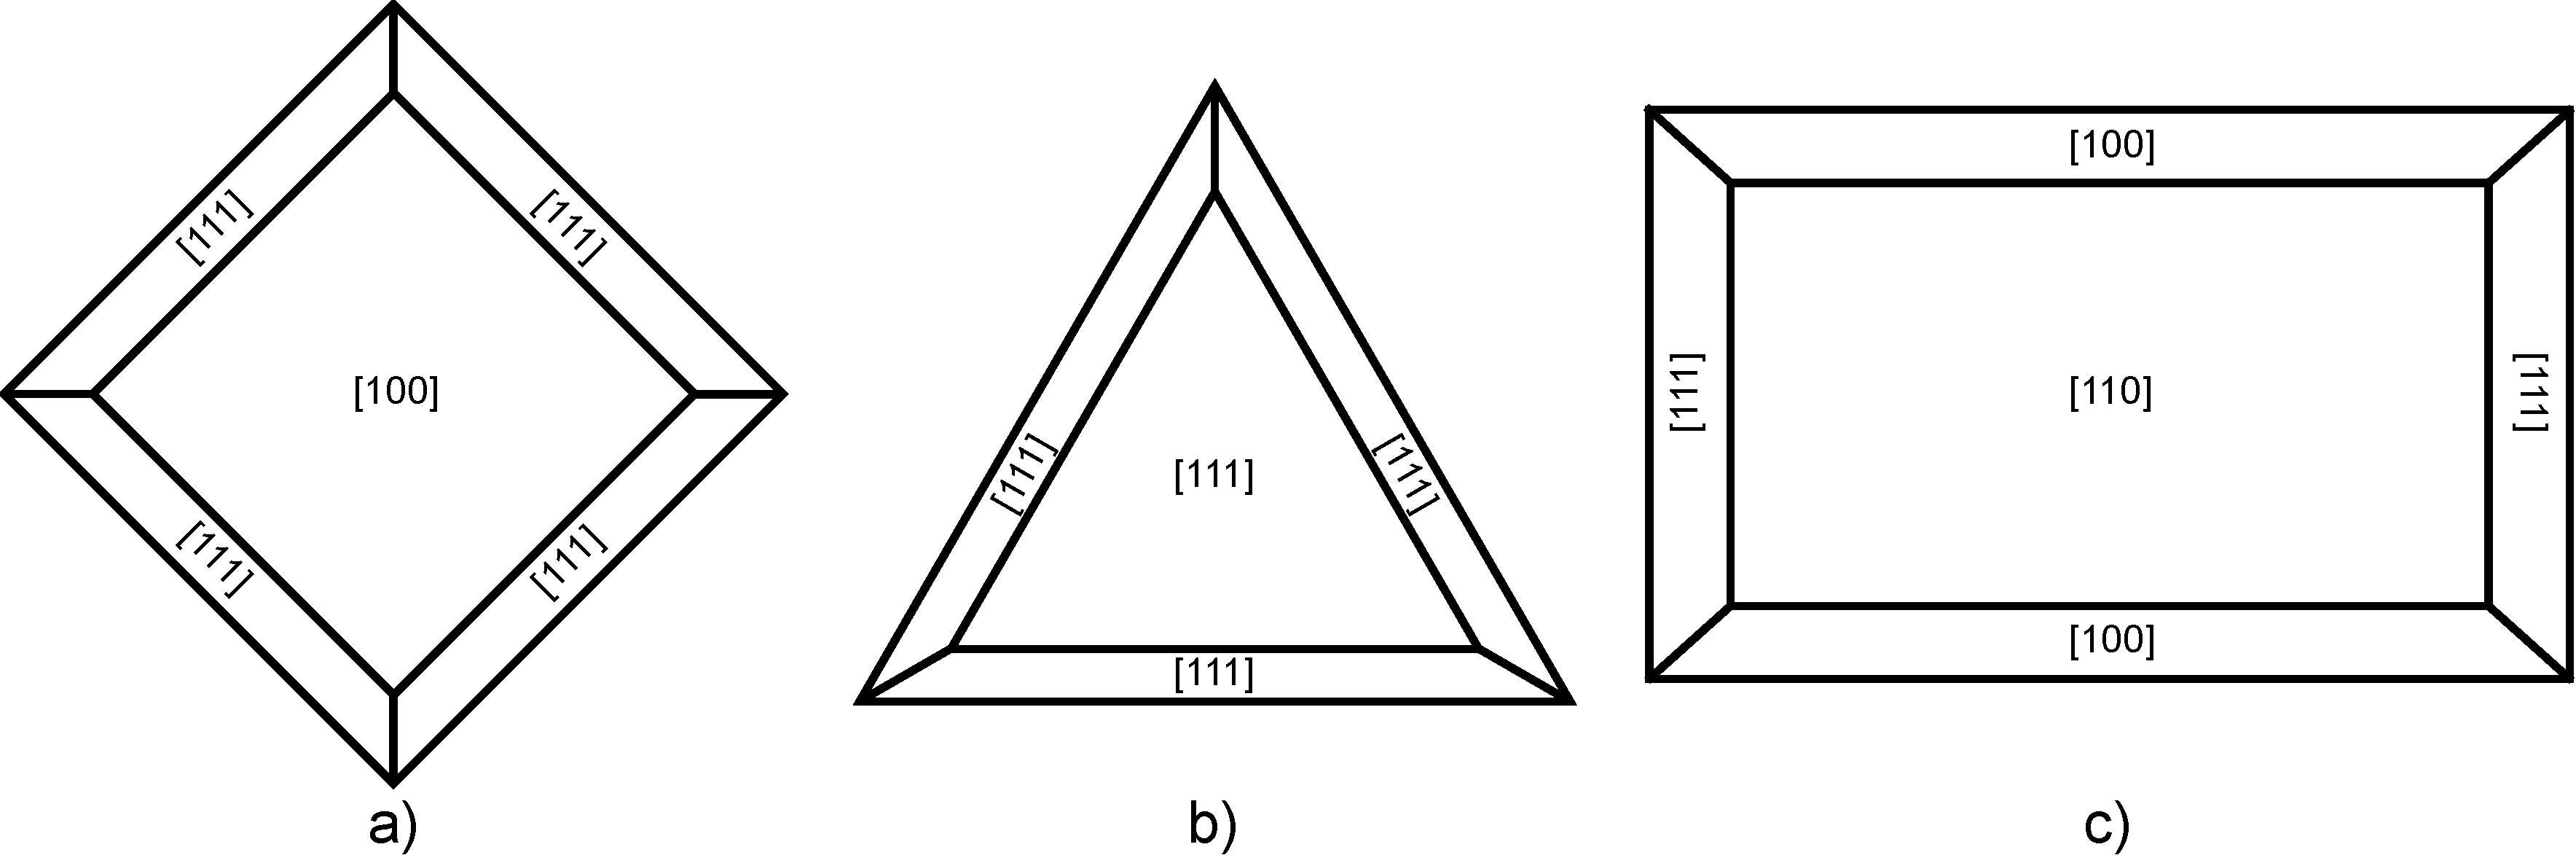
\includegraphics[width=\textwidth]{nanogold_facets}
    \caption[Model of gold nanostructure faceting]{\label{fig:nanogold_facets}Proposed faceting of the base structures grown on (a) [100]-, (b) [111]-, and (c) [110]-oriented substrates.}
\end{figure}
\begin{figure}
    \centering
    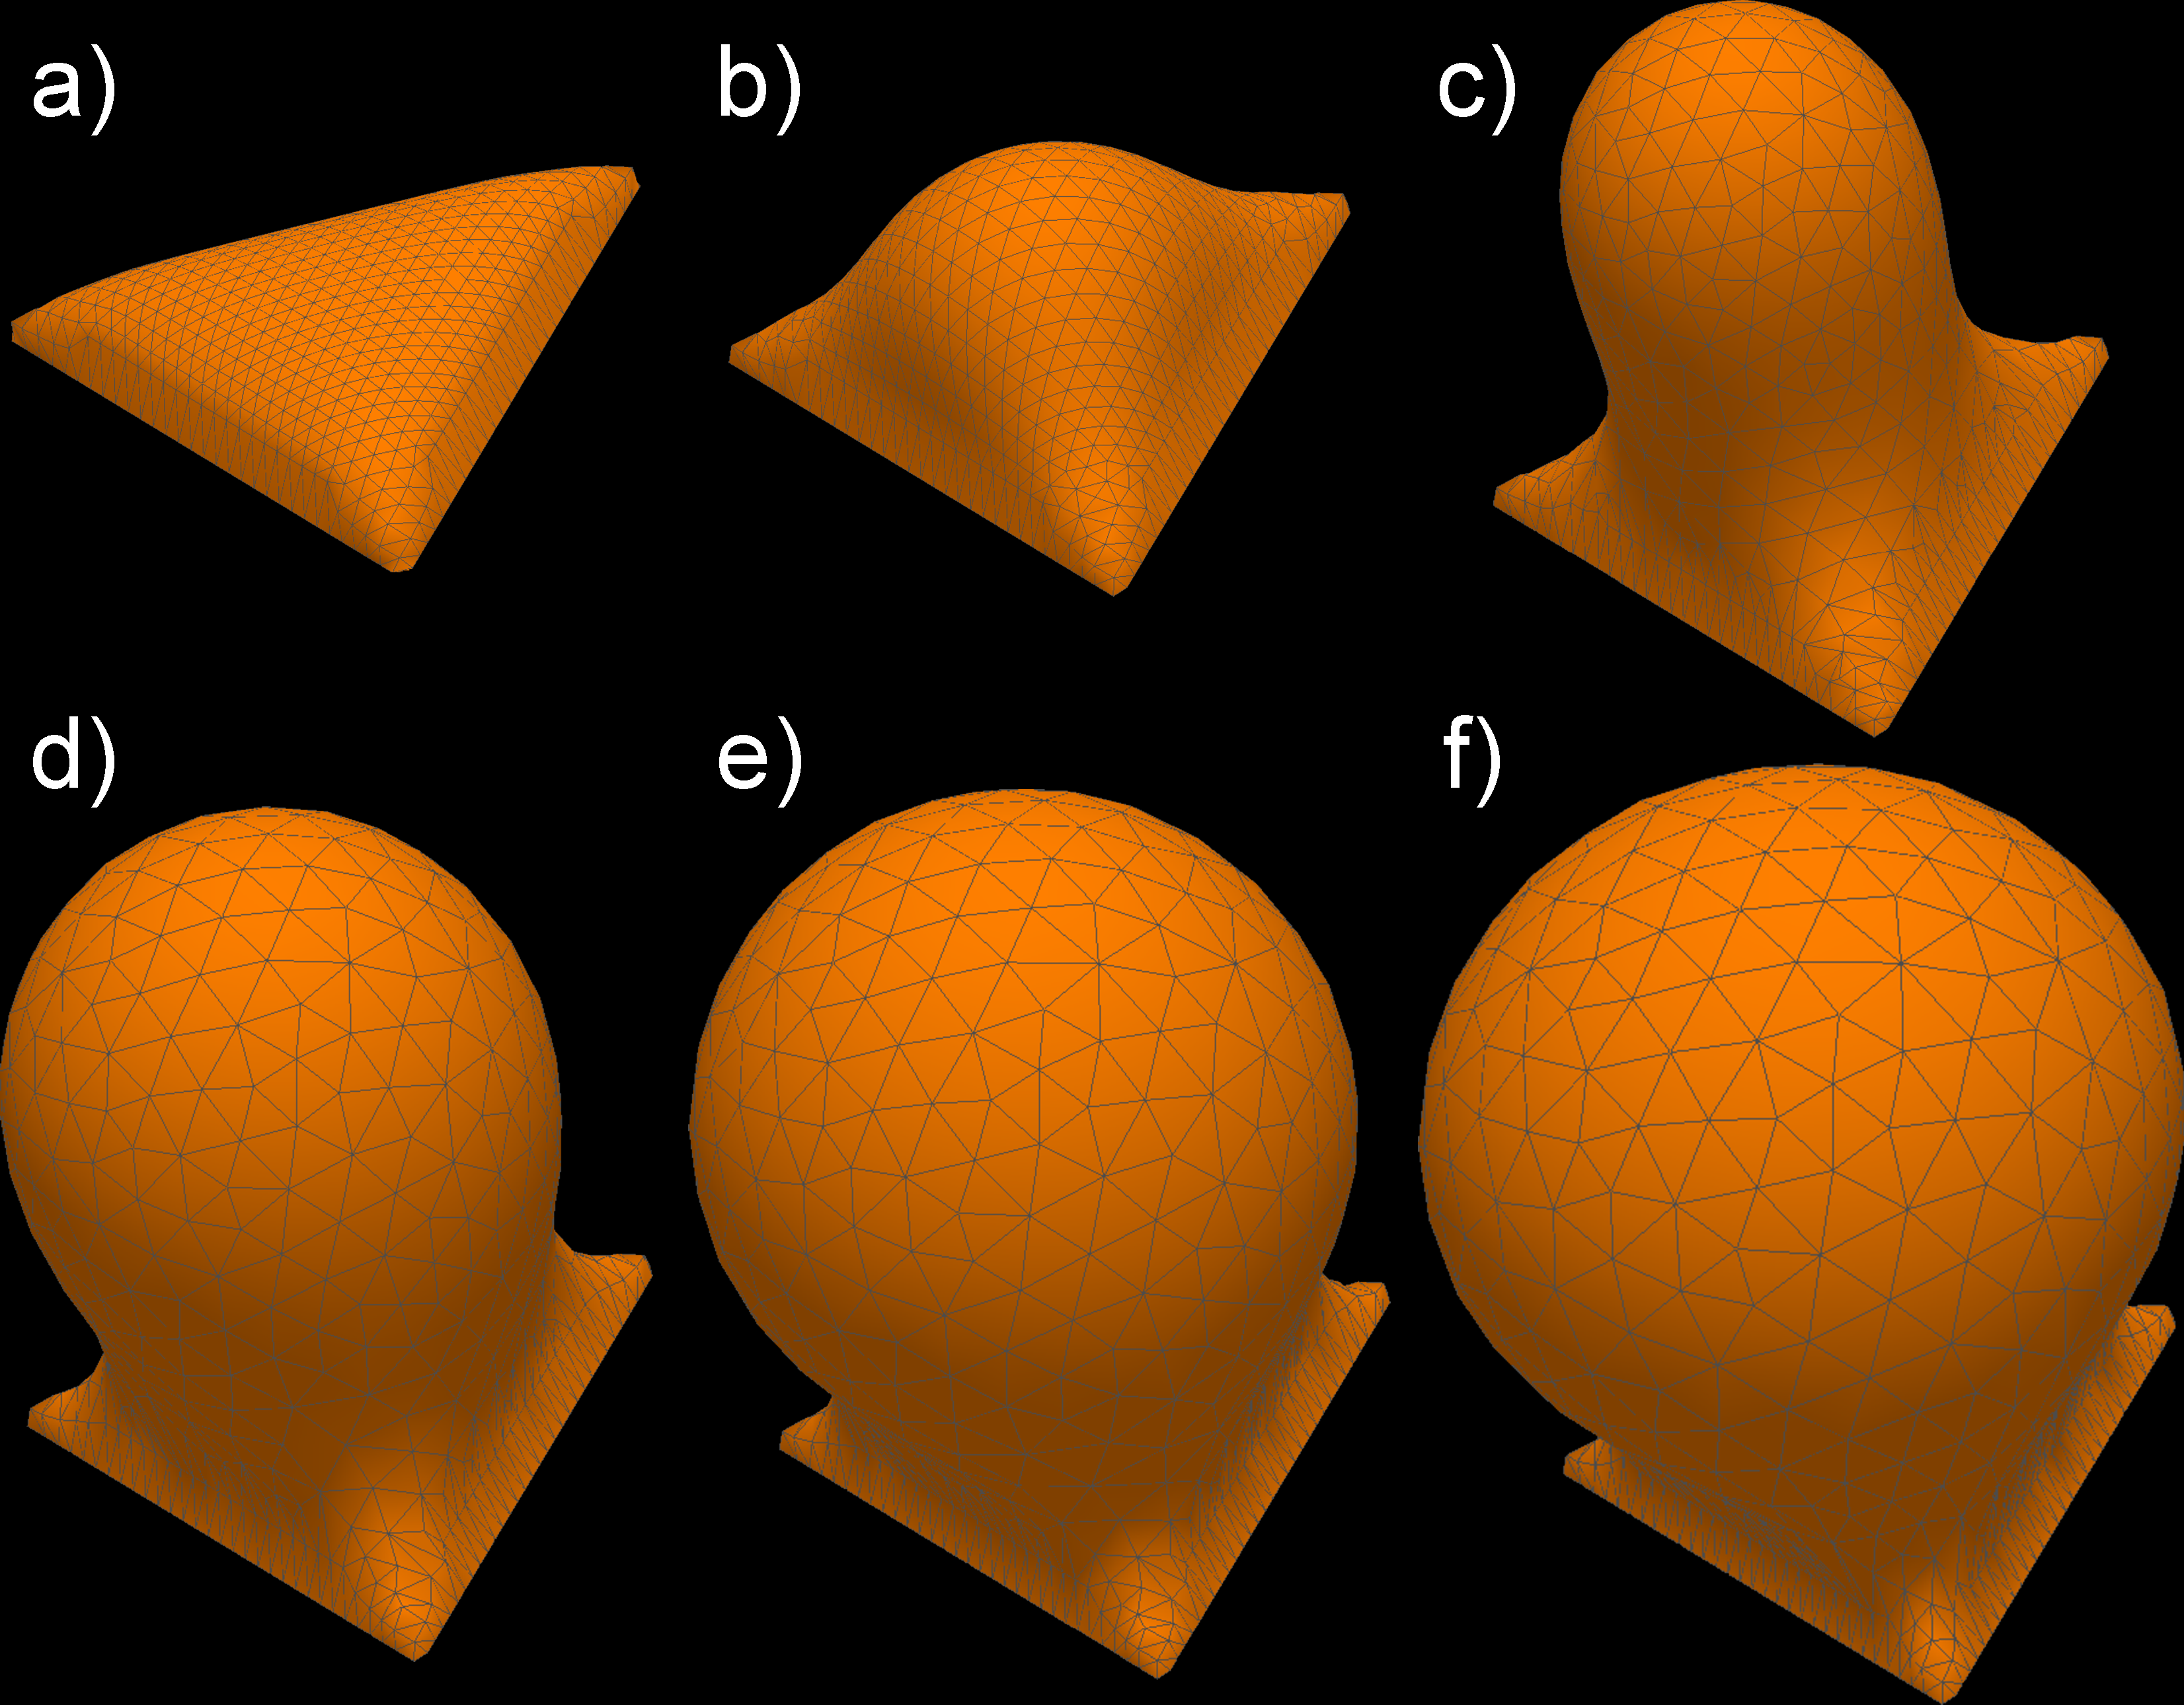
\includegraphics[width=\textwidth]{nanogold_simgrowth}
    \caption[Simulated gold nanostructure growth]{\label{fig:nanogold_simgrowth}Simulations based on the continuum elastic model showing the shape evolution of structures with a triangular footprint as the
        total volume is progressively increased. The shape of these modelled structures is remarkably similar to that of the self-assembled gold
        nanostructures formed on (111) MgAl\textsubscript{2}O\textsubscript{4} substrates (\protect{\cref{fig:nanogold_sem}}b and e and \protect{\cref{fig:nanogold_progression}}). The scale is in arbitrary units.}
\end{figure}

Using the numerical methodology, a progression of
structures with increasing volume were calculated using
square, triangular, and rectangular footprints having contact
angles of 54.7\degree, 70.5\degree, and 35\degree{} (long-axis) by 45\degree{} (short-axis),
respectively. The chosen contact angles are consistent with
the inferred faceting, as shown in \cref{fig:nanogold_facets}. For each case,
the footprint area and surface tension are set to unity, while
the bending modulus is allowed to vary. \cref{fig:nanogold_simgrowth} shows the
calculated progression for the triangular footprint. As the
volume is increased, there is an evolution from a nearly flat
base, to a base with a bulge, and then finally to a spherical
structure supported by a necked region to a triangular base.
These simulated structures are remarkably similar to the gold
nanostructures formed on the (111) MgAl\textsubscript{2}O\textsubscript{4} substrate (see
\cref{fig:nanogold_sem}b and c and \cref{fig:nanogold_progression}). Similar trends are observed for the
square and rectangular footprints. \Cref{fig:nanogold_square_rect} shows the
simulated high volume structures for the square and rectangular footprints, which, once again, are consistent with
experimental observations. The simulations do not, however,
account for any of the observed asymmetries.
\begin{figure}
    \centering
    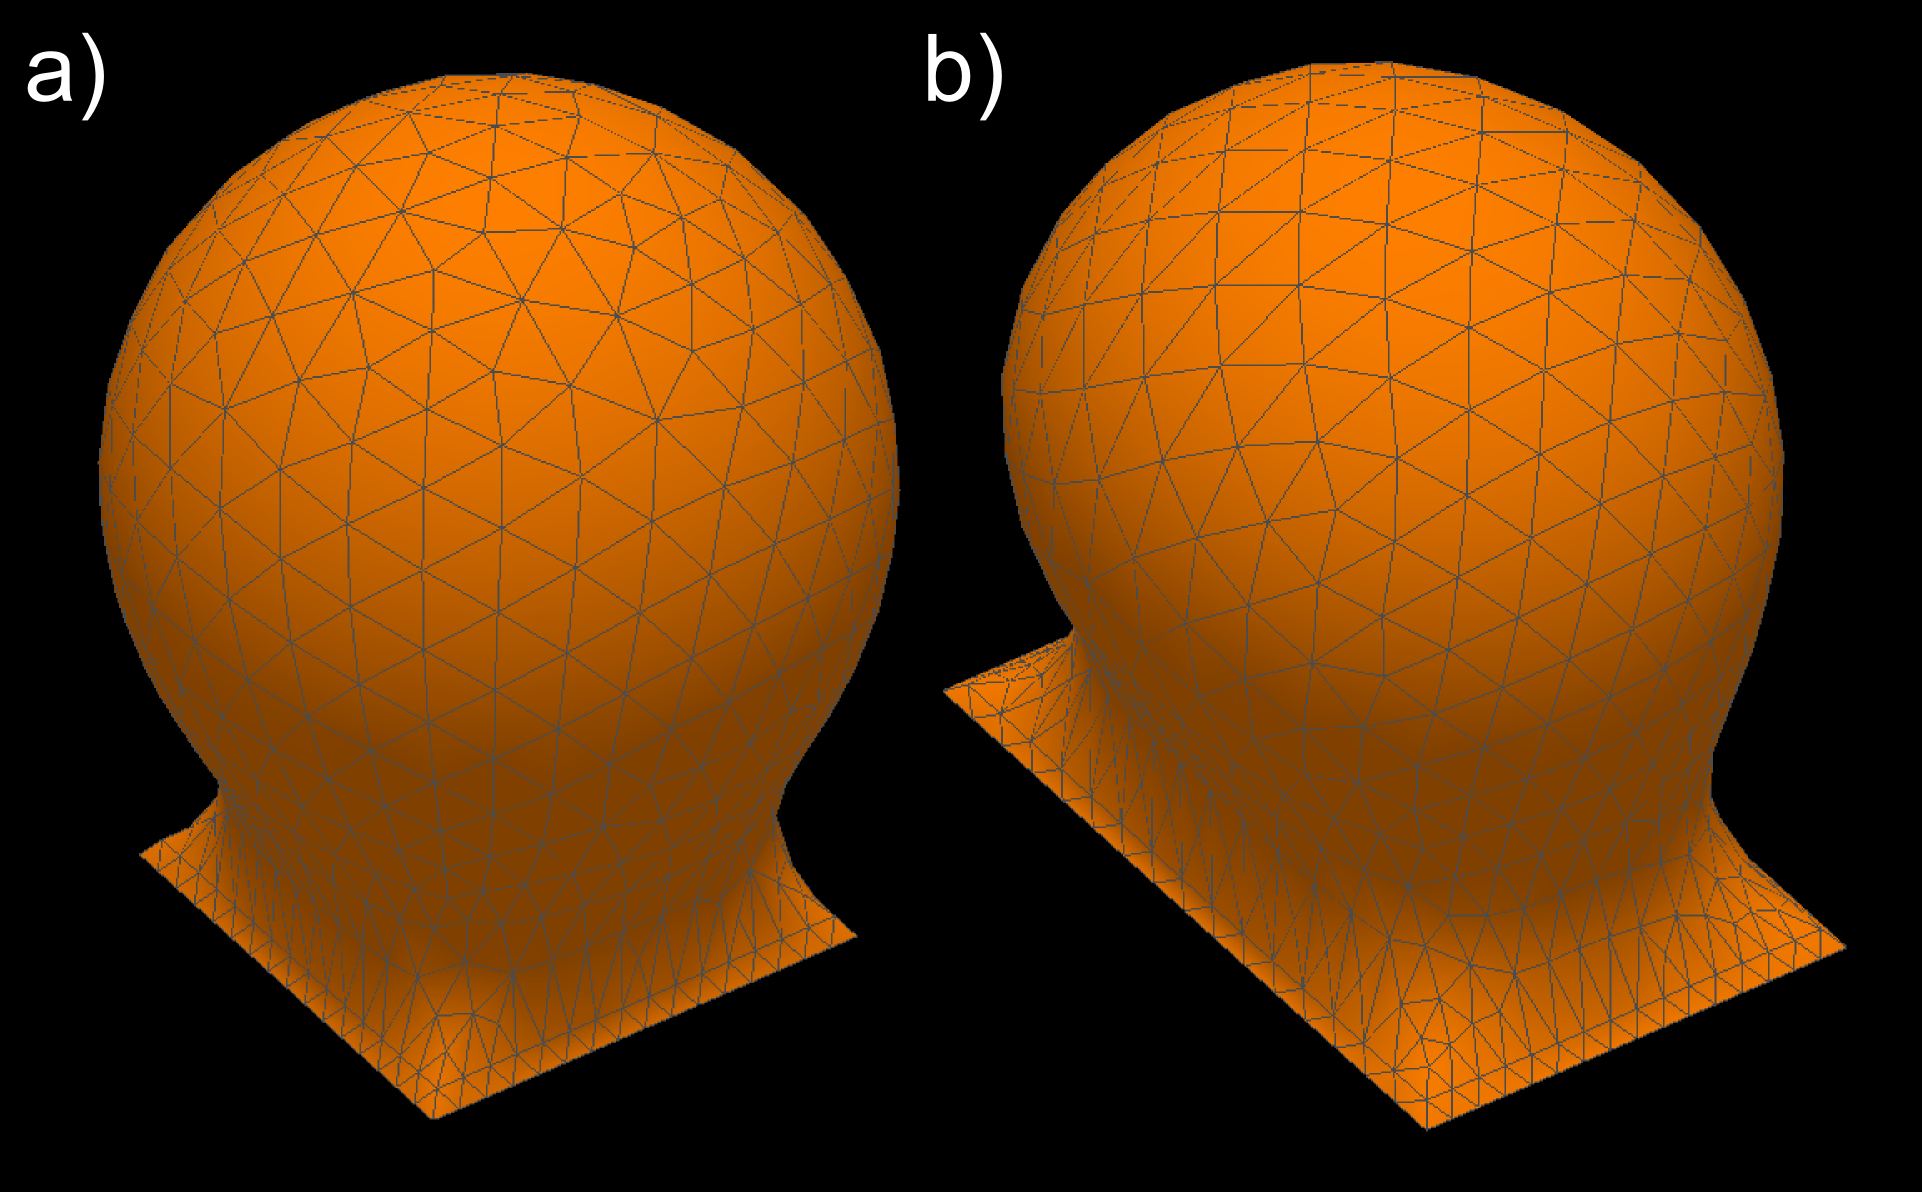
\includegraphics[width=\textwidth]{nanogold_square_rect}
    \caption[Simulations of square and rectangular base gold nanostructures]{\label{fig:nanogold_square_rect}Simulations based on the continuum elastic model
        showing the expected high volume shape for the (a) square and
        (b) rectangular (length/width ) 1.42:1) footprints. These structures
        show a resemblance to the self-assembled gold nanostructures
        formed on the (100) and (110) MgAl\textsubscript{2}O\textsubscript{4} substrates (\protect{\cref{fig:nanogold_sem}}) but
        show none of the observed asymmetries. The scale is in arbitrary
        units.}
\end{figure}

The shape of the base structures of the self-assembled gold
nanostructures is strongly influenced by epitaxy and the underlying symmetry of the substrate surface. That being
said, it is difficult to account for the hollowed-out center
observed for the base structure formed on the (100) MgAl\textsubscript{2}O\textsubscript{4}
using epitaxy-based arguments. This feature is, however,
predicted by the continuum elastic model. \Cref{fig:nanogold_afm}a shows
the topographical color map obtained from the modelling for
the low-volume structure. It clearly shows a circular depression in the middle of the structure as well as a lobe near
each corner. Motivated by the simulation results, we
examined the topography of the self-assembled gold nanostructure using atomic force microscopy (AFM). \Cref{fig:nanogold_afm}b
shows a tapping mode AFM image of the base structure
obtained using a Digital Instruments scanning probe microscope (SPM) and a NanoScope IIIa controller. Even though
the features of the nanostructure are somewhat washed out
due to the fact that the resulting image is a convolution of
the nanostructure and the AFM tip geometry, the nanostructure's four lobes and central depression are clearly visible.
\begin{figure}
    \centering
    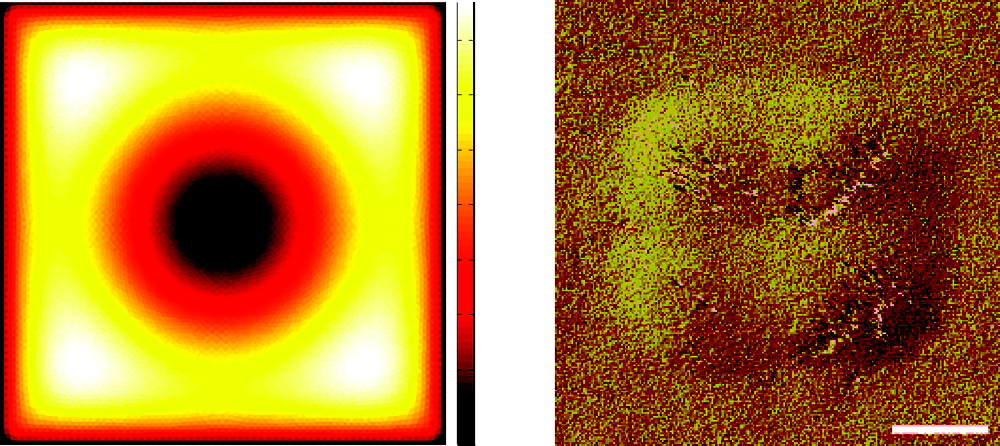
\includegraphics[width=0.8\textwidth]{nanogold_afm}
    \caption[Comparison of AFM and simulated gold nanostructure topography]{\label{fig:nanogold_afm}A comparison of the (a) topographical colour map derived
        from the continuum elastic model and (b) the AFM image of a
        self-assembled gold nanostructure deposited on the (100) MgAl\textsubscript{2}O\textsubscript{4}
        substrate. Note that the simulation predicts both the presence of
        four lobes at the corners and a central depression. The scale of the
        topographic image is arbitrary, and the scale of the AFM image is
        10 nm.}
\end{figure}

Taken together, the experimental observations and the
continuum elastic modelling results strongly suggest that
epitaxy and a minimization of the surface free energy are
the two primary drivers in determining the shape and size
of the self-assembled gold nanostructures. The fact that
similar structures have not been previously observed is likely
a consequence of the synthesis route used. The route employed here not only involves temperatures well in excess
of those typically used when forming substrate-supported
nanostructures but also requires an annealing profile which
accesses two temperatures. It is possible that the initial 1100 \celsius~anneal is needed to induce surface reconstructions in the
MgAl\textsubscript{2}O\textsubscript{4} substrates which are essential to the growth of these
nanostructures. Surface reconstructions have been shown to
strongly influence the growth of both nanostructures\cite{RefWorks:24,RefWorks:16,RefWorks:104}
and thin films\cite{Neretina2009a} when using (100) SrTiO3 substrates. We,
however, consider it more likely that the formation of these
nanostructures requires temperatures in excess of the melting
point of bulk gold (1064 \celsius). Significant deviations from
the bulk value, due to finite size effects, are considered
unlikely since such effects appear to occur only in nanostructures smaller than 5 nm\cite{RefWorks:43}. Once molten, the nanostructures are cooled to 1000 \celsius~and held at this temperature,
which is just below the melting point. Such a temperature
allows for solidification while maintaining high adatom
mobility. The fact that this fabrication step is crucial to the
formation of the observed intricate nanostructures provides
compelling evidence that considerable adatom motion is
essential. In this scenario, it is likely that an Ostwald-like
ripening process will play a role where larger nanostructures
grow at the expense of smaller ones. Substrate surface steps,
due to the inherent miscut of the substrate\cite{RefWorks:69}, could also
influence the process by providing energetically favorable
nucleation sites. Nanostructure formation is also heavily
reliant on the epitaxial relationship between the nanostructure
base and the underlying substrate. This relationship determines the crystallographic alignment of the base structures,
while the consistency in size is likely a consequence of the
strain imposed by lattice mismatch. Once the 1000 \celsius~anneal
ends, the adatom motion will be quickly quenched by the
lower temperatures, allowing no further alterations to the
shape or size of the nanostructures. The end result is
intricately shaped nanostructures whose size and shape are
determined by a minimization of the surface free energy
while simultaneously being subject to the constraints imposed
by epitaxy.
\section{Implications for Symmetry and Energy at Epitaxial Surfaces}
Despite the materials of interest in this investigation consisting of a noble metal and a complex oxide, materials which one would not expect any kind of interaction, result in epitaxial alignment. This epitaxial alignment is simple in the sense that the nanocrystal orientations follow directly from the underlying substrate. The epitaxial alignment is complicated by the fact that gold fits onto  sublattice of half of a MgAl\textsubscript{2}O\textsubscript{4} lattice. Such epitaxy relies on the symmetry of the surface atoms forming a lattice with a smaller lattice constant than the bulk crystal. This epitaxy can thus be thought of as nanocrystal forming on a reconstructed surface, since the surface atoms present a surface net with a different lattice parameter than the bulk.

The more surprising result from this work is the epitaxial alignment possible between very nonreactive materials. Noble metals are not known to readily react with other elements or compounds other than to form simple metallic bonds. Similarly, metals in general are not known to strongly wet oxide surfaces, preferring to bond to themselves instead. Complex oxides are also known to be very stable to high temperatures, and stable to a great many compounds. To mix such two compounds and observe something other than segregation and no interaction is surprising. These experiments have shown that, despite there being a very weak interaction between the two materials, due to low reactivity, epitaxial alignment is achieved through a careful thermal treatment. The subtle influence of the substrate's lattice can impart alignment of the gold, overriding the tendency to form a equilibrium crystal shape.


%%Other useful examples
%\textsubscript{} and \textsuperscript{} are the best way to do super/sub (provided by fixltx2e)

\printbibliography
%\printindex
\end{document}
